%%%---PREAMBLE---%%%%%%%%%%%%%%%%%%%%%%%%%%%%
\documentclass[oneside,12pt,final]{/Applications/TeX/packages/ucthesis-CA2012}
%if twoside use 
%\raggedbottom
\pdfoutput=1

%--- Packages ---------------------------------------------------------
%\usepackage[lofdepth,lotdepth,caption=false]{subfig}
\usepackage{subfigure}
\usepackage{fancyhdr}
\usepackage{hyperref}
\usepackage{amsmath, amssymb, graphicx}
\usepackage{xspace}
\usepackage{braket}
\usepackage{color}
\usepackage{setspace}
\usepackage{listings}
\lstset{basicstyle=\ttfamily,
escapeinside={||},
mathescape=true}

%\usepackage{tabu}
\usepackage{dcolumn}
\newcolumntype{d}[1]{D{.}{.}{#1}}

%\usepackage{subfigure} (Subfigure package clashes with another package)

%---New Definitions and Commands------------------------------------------------------
\def\p{\partial}
\def\im{\mrm{im}}
\def\Tr{\mrm{Tr}}
\def\Z{\mbb{Z}}
\def\R{\mbb{R}}
\def\C{\mbb{C}}
\def\half{\frac{1}{2}}
\def\filler{\phantom{fillerfillerfiller}}
\newcommand{\be}{\begin{equation}}
\newcommand{\ee}{\end{equation}}
\newcommand{\mbb}[1]{\mathbb{#1}}
\newcommand{\mrm}[1]{\mathrm{#1}}
\newcommand{\mcal}[1]{\mathcal{#1}}
\newcommand{\mbf}[1]{\mathbf{#1}}
\newcommand{\ph}[1]{\phantom{#1}}
\newcommand{\udten}[3]{#1^{#2}_{\ph{#2}#3}}
\newcommand{\duten}[3]{#1^{\ph{#2}#3}_{#2}}
\newcommand{\pd}[2]{\frac{\p#1}{\p#2}}
\newcommand{\D}[2]{\frac{d#1}{d#2}}

%---Set Margins ------------------------------------------------------
%\setlength\oddsidemargin{0.25 in} \setlength\evensidemargin{0.25 in} \setlength\textwidth{6.25 in} 
\setlength\oddsidemargin{0.25 in} \setlength\evensidemargin{0.25 in} \setlength\textwidth{6.15 in} 


\setlength\textheight{8.50 in}
\setlength\footskip{0.25 in} \setlength\topmargin{0 in} \setlength\headheight{0.25 in} \setlength\headsep{0.25 in}

%%%---DOCUMENT---%%%%%%%%%%%%%%%%%%%%%%%%%%%%
\begin{document}
%=== Preliminary Pages ============================================
\begin{frontmatter}
	%%%%%%%%%%%%%%%%%%%%%%%%%%%
% TITLE PAGE INFORMATION %
%%%%%%%%%%%%%%%%%%%%%%%%%%%


\title{A Level-Set Approach for Simulating Dendritic Crystal Growth}

\author{Megan Maria Chang}

%%%%%%%%%%%%%%%%%%%%%%%%%%%%%%%%%%
% DECLARATIONS FOR FRONT MATTER %
%%%%%%%%%%%%%%%%%%%%%%%%%%%%%%%%%%
\report{Thesis} \degree{Master of Science} \degreemonth{June} \degreeyear{2017}
\defensemonth{March}
\defenseyear{2017}

\chair{Professor Frederic Gibou} \othermemberA{Professor Paolo Luzzatto-Fegiz} \othermemberB{Professor Jeffrey Moehlis}   \numberofmembers{3}

\field{Mechanical Engineering}
\campus{Santa Barbara}


%\title{{ University of California \\ Santa Barbara} \linebreak \\  Ph.D. Dissertation}
%\author{Tom\'as Andrade}
%\date{2012}

	\maketitle
	\approvalpage
	\copyrightpage
	%\begin{dedication}

\bigskip

${}$ \\

\bigskip

${}$ \\

\bigskip

${}$ \\

\bigskip

\begin{center}
\begin{Large}
Dedication here
\end{Large}
\end{center}


\end{dedication} %comment out if you don't want a dedication
	\begin{acknowledgements}

First and foremost, I offer my sincerest gratitude to my graduate research advisor, Dr. Frederic Gibou, Professor of Mechanical Engineering UCSB, for his unwavering encouragement and guidance. I thank Raphael Egan for his patience and for taking me under his computational wing. I thank my parents for their wise counsel and sympathetic ear. And I thank my friends who kept me sane throughout the crazy ride that is graduate school. 

\end{acknowledgements} 
	%\begin{vitae}

\begin{vitaesection}{Education}
\vspace{-0.1cm}
\item [2017]	M.S. in Mechanical Engineering (Expected), University of California, Santa Barbara.
\item [2015]	B.S. in Mechanical Engineering, University of California, Santa Barbara.
\end{vitaesection}

%\textbf{Publications}

%Publications.

\end{vitae}
	%
%  Abstract
%

\begin{abstract}
%todo: max 350 words

In this thesis, we consider the piecewise constant coefficient Stefan problem, a free boundary problem described by a partial differential equation with an unknown concentration $u$ and an unknown time-dependent irregular domain $\Omega^-$, used primarily to study phase transitions. We present a numerical method for solving the two-dimensional, unsteady, two-phase, diffusion equation on an irregular domain with Dirichlet boundary conditions at the solidification front. Several techniques were implemented to achieve this including: the implicit level-set method to update the location of the interface and keep track of the two phases it separates; the Ghost-Fluid method to impose boundary conditions on an irregular domain and allow for symmetric discretization of our diffusion matrix; a third-order extrapolation method to allow for both accurate interface velocity calculations and implicit discretization by providing valid values at grid points that may be contained in $\Omega^-$ in the next time step; a combination of WENO spatial discretization and TVD RK3 time discretization to achieve third-order accurate advection; and finally for diffusion, we implemented the Crank-Nicholson method to achieve second-order accuracy in both space and time with implicit time stepping. Overall, for the Stefan problem, we demonstrate that through robust and computationally efficient methods, it is possible to simulate complex dendritic crystal growth.

%\abstractsignature
\end{abstract}



	\tableofcontents
	\listoffigures
	\listoftables
\end{frontmatter}

\begin{mainmatter}

%---Set Headers and Footers ------------------------------------------------------
\pagestyle{fancy}
\renewcommand{\chaptermark}[1]{\markboth{{\sf #1 \hspace*{\fill} Chapter~\thechapter}}{} }
\renewcommand{\sectionmark}[1]{\markright{ {\sf Section~\thesection \hspace*{\fill} #1 }}}
\fancyhf{}

\makeatletter \if@twoside \fancyhead[LO]{\small \rightmark} \fancyhead[RE]{\small\leftmark} \else \fancyhead[LO]{\small\leftmark}
\fancyhead[RE]{\small\rightmark} \fi

\def\cleardoublepage{\clearpage\if@openright \ifodd\c@page\else
  \hbox{}
  \vspace*{\fill}
  \begin{center}
    This page intentionally left blank
  \end{center}
  \vspace{\fill}
  \thispagestyle{plain}
  \newpage
  \fi \fi}
\makeatother
\fancyfoot[c]{\textrm{\textup{\thepage}}} % page number
\fancyfoot[C]{\thepage}
\renewcommand{\headrulewidth}{0.4pt}

\fancypagestyle{plain} { \fancyhf{} \fancyfoot[C]{\thepage}
\renewcommand{\headrulewidth}{0pt}
\renewcommand{\footrulewidth}{0pt}}

%=== Introduction ============================================
\chapter{Introduction}

The Stefan problem is a free boundary problem that describes the motion of a front driven by diffusion, making it highly useful for analyzing phase transitions. For example, the Stefan problem is used in thermodynamics to study crystal growth in a supercooled solution; in materials science to study the mixture of molten metals and elements to create alloys with superior properties; and in biomedicine to study cancer invasion and tumor growth. Its plethora of applications concerning diffusion-dominated phenomena have made it an important model to study.

The governing equations of the Stefan problem are: diffusion, which is the driving force of our phase transition; the Gibbs-Thomson boundary condition, which imposes anisotropic behavior that leads to dendritic growth; and the interface velocity calculation used to move our level-set and update the interface location through advection. These three equations are given by

\begin{equation}\label{eqn:governing}
\begin{aligned}
\text{Diffusion:}& \quad \frac{\partial u}{\partial t} = D \Delta u,\\
\text{Gibbs-Thomson BC:}&\quad u_\gamma = u + \epsilon \kappa,\\
\text{Interface Velocity:}&\quad \vec{v} = [D \nabla u]_{\gamma}, 
\end{aligned}
\end{equation}
where $\Delta$ is the Laplace operator (a second-order differential operator), and $\nabla$ is the gradient (a first-order differential operator), $u$ is the concentration, $u_{\gamma}$ is the concentration at the front, $t$ is real time, $D$ is the diffusion coefficient, $\epsilon$ is the anisotropy strength, $\kappa$ is the curvature, $\vec{v}$ is the interface velocity, and $[\cdot]_\gamma$ denotes a jump across the interface.

The most common example of dendritic crystal growth is the snowflake, where the dendrites refer to the branches of the tree-like structure. Since there are no existing analytical methods for solving and predicting dendritic crystal growth, we rely on numerical methods to tackle these complicated problems. A successful method should be able to track a moving solid-liquid interface undergoing complex topological changes, and must be computationally efficient since these methods often require high grid resolutions, in order to capture these dendrites, and strict time step restrictions to ensure stability.

Several techniques are used in practice to track a time-evolving boundary, or interface. These methods can be described as either explicit tracking or implicit capturing. Explicit methods such as front tracking are valued for their accuracy, but fall short when it comes to handling topological changes such as materials merging or separating. In the case where a material melts and develops holes, or else experiences crystal growth such that dendrites begin to merge, additional numerical treatment is required. One would need to develop an algorithm that could detect the moment objects merged or separated and construct new parameterizations to describe each newly separated or joined shape, a very challenging task.

Alternatively, implicit methods such as the level-set method represent the interface as an isocontour of a Lipschitz continuous function. This allows for straightforward handling of topological changes, since objects do not have to be parametrized. As we move from two-dimensional objects to three-dimensional objects, this becomes increasingly important. The main drawback of the level-set method is that it is less accurate in terms of mass conservation. However in [2], Min and Gibou address this problem with adaptive grids and demonstrate its ability to alleviate this problem of mass loss or gain.

Since we are interested in developing a method which can simulate complicated dendritic crystal growth, we employ the level-set method paired with the Ghost-Fluid method to achieve a superior interface capturing scheme.

%%%%%%%%%%%%%%%%%%%%%%%%%%%%%%%%%%%%%%%%%%%%%%%%%%%%%%%
%%%%%%%%%%%%%%%%%%%%%%%%%%%%%%%%%%%%%%%%%%%%%%%%%%%%%%%
The level-set advection equation
\begin{equation} \label{eqn:level_set}
\begin{aligned}
\phi_t + \vec{v} \cdot \nabla \phi = 0
\end{aligned}
\end{equation}
is a PDE which uses a higher dimensional level-set function $\phi$ to describe the motion of a co-dimension 1 shape, under a velocity field $\vec{v}$. In this thesis, we use a three-dimensional level-set function $\phi$ to keep track of a two-dimensional shape, where the zero-contour represents the interface separating two materials.

Henceforth, in a domain $\Omega$, we can refer to the region where $\phi < 0$ as reacted material, or the subdomain $\Omega^-$; and refer to the region where $\phi > 0$ as unreacted material, or the subdomain $\Omega^+$. These two substances are separated by the interface, where $\phi = 0$, across which unreacted material can be converted into reacted material or vice versa (i.e. ice in water begins to melt into more water, or supercooled water surrounding ice begins to freeze into more ice). The labels reacted vs. unreacted hold no physical implication, they are simply a nominal tool used to distinguish whether we are in the negative $\phi$ subdomain (i.e. $\Omega^-$) or the positive $\phi$ subdomain (i.e. $\Omega^+$). That is to say the reacted material could refer to either ice or water, as you prefer.

This is an important fact to keep in mind because throughout the thesis, we will discuss how to solve only in $\Omega^-$. However, this \textbf{does not} mean we are ignoring the material in $\Omega^+$. On the contrary, both subdomains are of equal importance in simulating crystal growth. We simply ignore $\Omega^+$, while we solve in $\Omega^-$, then ignore $\Omega^-$ while we solve in $\Omega^+$ using the exact same methods. Decoupling the two solutions is a useful simplification we can make since we are given Dirichlet boundary conditions. Thus, to solve for diffusion in each subdomain, our governing equation becomes
\begin{equation}\label{eqn:governing_diff}
\begin{aligned}
\text{Diffusion in $\Omega^-$:}& \quad \frac{\partial u_\text{in  } \>}{\partial t} = D_\text{in  }\> \Delta u_\text{in  },\>\\
\text{Diffusion in $\Omega^+$:}& \quad \frac{\partial u_\text{out}}{\partial t} = D_\text{out} \Delta u_\text{out},\\
\end{aligned}
\end{equation}
where $D_\text{in}$ and $u_\text{in}$ represent values in $\Omega^-$, while $D_\text{out}$ and $u_\text{out}$ represent values in $\Omega^+$. And the governing interface velocity calculation becomes
\begin{equation}
\vec{v} = D_\text{in} \nabla u_\text{in} - D_\text{out} \nabla u_\text{out}
\end{equation}
to appropriately represent the meeting of the two subdomains at the interface.
%%%%%%%%%%%%%%%%%%%%%%%%%%%%%%%%%%%%%%%%%%%%%%%%%%%%%%%
%%%%%%%%%%%%%%%%%%%%%%%%%%%%%%%%%%%%%%%%%%%%%%%%%%%%%%%

To build the most efficient solver requires \textbf{symmetric} matrix discretization. This symmetry allows us to use fast matrix inversion methods like the Preconditioned Conjugate Gradient (PCG) method. Since we build a diffusion matrix that is symmetric and positive definite, the Matlab backslash operator can select the Choleski triangular solver to precondition our matrix.

Previous methods, for analyzing the Stefan problem, sacrificed this symmetry to achieve second-order accuracy by implementing higher-order extrapolation to compute ghost values. However, in [1], Gibou and Fedkiw show that using only linear and constant extrapolation to calculate ghost values, rather than quadratic leads to a symmetric discretization that is still second-order accurate in the solution of $u$, but loses second-order accuracy in the gradient (i.e. $\nabla u$). This means our Stefan solver would become first-order accurate due to the gradient calculations in the interface velocity computation. However, we choose computational efficiency over second-order accuracy since this non-symmetric discretization becomes computationally prohibitive at higher grid resolutions. Thus, we implement ghost values using linear extrapolation.

Our computational grid is made up of cells of width $\Delta x$ and height $\Delta y$. The cell centers are known as grid points or grid nodes with the $i$th grid node located at $x_i$ and the $j$th grid node located at $y_j$. The value of interest at each cell is concentration, denoted as $u_{i,j}$ at some location ($x_i,y_j$). Further, we use the superscript $n$ to describe our time at some $t^n$, such that the initial conditions would be described as $u_{i,j}^0$. 

In order to capture dendritic growth, these Stefan problems often require very fine grid resolutions. Since our time step restriction is dependent on the spatial grid size, we want to minimize this dependency by using \textbf{implicit} time stepping in our diffusion discretization to allow our time step $\Delta t$ to be proportional to $\Delta x$, as opposed to $\Delta t$ being proportional to $\Delta x^2$, as is the case with explicit time stepping. This way, as we refine our grid from a resolution of 100$\times$100 to 200$\times$200, the time step will shrink by a factor of $\frac{1}{2}$ instead of $\frac{1}{4}$, and as we move from a resolution of 100$\times$100 to 400$\times$400, the time step will shrink by a factor of $\frac{1}{4}$ instead of $\frac{1}{16}$. It is important to note that the implicit level-set method enables us to use implicit discretization, here, as well. Hence, we employ the Crank-Nicholson scheme so that $\Delta t$ can be equal to $\Delta x$. This means our time step will be limited by advection where we will implement a Courant-Friedrichs-Lewy (CFL) number of 0.5, such that
\begin{equation}\label{eqn:time_step_restriction_1}
\Delta t = \frac{0.5 \text{min} (\Delta x,\Delta y)}{|v|_{max}},
\end{equation}
where $\Delta t$ represents a real physical time step used in the diffusion and advection steps, and $|v|_{max}$ is the maximum interface velocity. This $\Delta t$ must be recalculated at every time step since $|v|_{max}$ will be constantly changing.

This implicit Crank-Nicholson scheme may require the use of extrapolated values. Consider the case where between time steps $t^n$ and $t^{n+1}$, the interface moves so that a point $u_{i,j}$ contained in $\Omega^+$ is now contained in $\Omega^-$. In the Crank-Nicholson scheme, we would need a valid value at that point for $u^n_{i,j}$ and $u^{n+1}_{i,j}$. However, this value for $u^n_{i,j}$ would not exist, since it was not contained in $\Omega^-$ at $t^n$, and as we said before, the solutions in each subdomain are decoupled. For this reason, we need to employ a third-order extrapolation method to extrapolate values of $u^n$ in the layer of grid nodes near the interface.

This third-order extrapolation method is also necessary for computing gradient calculations at the interface to determine the interface velocity (\ref{eqn:governing}c). Gradient calculations in two-dimensions are given by 
\begin{equation}
\nabla u  = \bigg( u_x, u_y \bigg) =\>\>  \bigg( \> \frac{\partial u}{\partial x},\frac{\partial u}{\partial y} \> \bigg),
\end{equation}
where $\nabla$ is the symbolic representation of the gradient field. In derivative notation, the subscript denotes the partial differential of a function $u$ with respect to either $x$ or $y$. This is not to be confused with our $u_{i,j}$ subscript notation to describe spatial location.

For this extrapolation method, as well as for the constant extrapolation and reinitialization methods, a new fictitious time step restriction must be satisfied to ensure numerical stability. This fictitious time step,
\begin{equation}\label{eqn:time_step_restriction_2}
\Delta \tau = 0.5 \text{min} (\Delta x,\Delta y),
\end{equation}
is used to reach a steady state solution in our iterative methods. This will become more clear as we discuss each method in the later sections. However, we mention this, now, because it is important to keep in mind that there are two separate time step restrictions used in this paper that are not to be confused.

Throughout this thesis, we analyze errors using the standard mathematical \textit{p-norm}
\begin{equation}
||\vec{x}||_{p} = \bigg({\displaystyle \sum_{k=1}^{N}  |x_{k}|^{p} }\bigg)^{\frac{1}{p}},
\end{equation}
where the scalar $x_k$ refers to the error $u_\text{exact} - u_\text{numerical}$ at every point in the domain. To be thorough, we consider the $L^1$ norm and the $L^\infty$ norm, where $L^1$ is the sum of the absolute values of error multiplied by the grid size area, and $L^\infty$ returns the maximum absolute value of error. Thus, $L^1$ gives us a good sense of the overall accuracy of our solvers across the entire domain, and $L^\infty$ warns us if there is any one point in the domain that is giving rise to more error such as, for instance, at the front. When we plot these errors against the grid size on a log-log plot, the slope tells us the order of accuracy of our scheme, where the order quantifies the rate of convergence of our numerical approximation to the exact solution. If a method is said to be second-order accurate, one would expect the error to reduce by a factor of 4 if the grid resolution increased from 100$\times$100 to 200$\times$200, and reduce by a factor of 16 as we move from a resolution of 100$\times$100 to 400$\times$400. To provide this data in a more concise form, rather than plots, we can use 
\begin{equation}\label{eqn:order}
\begin{aligned}
\text{Order} \>= \text{log}_2\bigg(\frac{L^1 \text{ error using $\Delta x$}}{L^1 \text{ error using $\frac{\Delta x}{2}$}}\bigg)
\end{aligned}
\end{equation}
to calculate the order of accuracy, where the base of log$_2$ comes from the fact that the grid resolutions double each time we refine the grid. To be specific and consistent, we use grid resolutions 81$\times$81, 161$\times$161, and 321$\times$321 for all of our accuracy testing.

%=== Chapter 2  ============================================
\chapter{The Level-Set Method}\label{section:Level_Set_Method}

In Figure \ref{fig:level_set_1}, we demonstrate how the three-dimensional level-set allows us to easily keep track of the interface separating reacted and unreacted material. Notice, we have inverted the $z$- axis so that $\phi$ is positive downwards, for better visual representation. Following this, we included Figure \ref{fig:level_set_2} to demonstrate the real power of the level-set method: its ability to handle complex topological changes such as melting into separate pieces or conversely, pieces growing and merging together.

\begin{figure} [!h]
\centering
\subfigure[$\phi$]{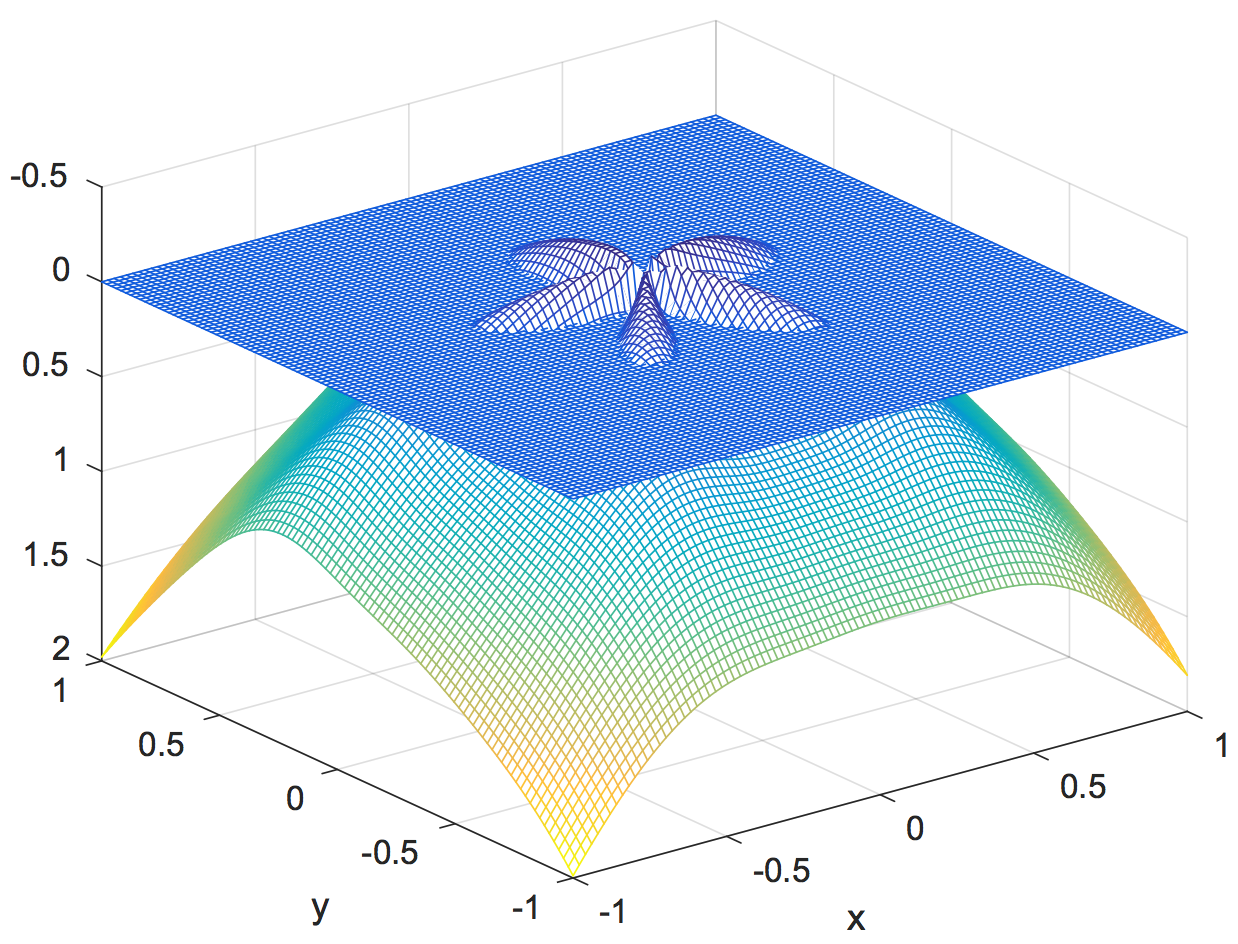
\includegraphics[width=.42\textwidth]{/Users/meganchang/Desktop/Thesis/images/Level_Set_1.png}} \quad
\subfigure[$\Omega^-$]{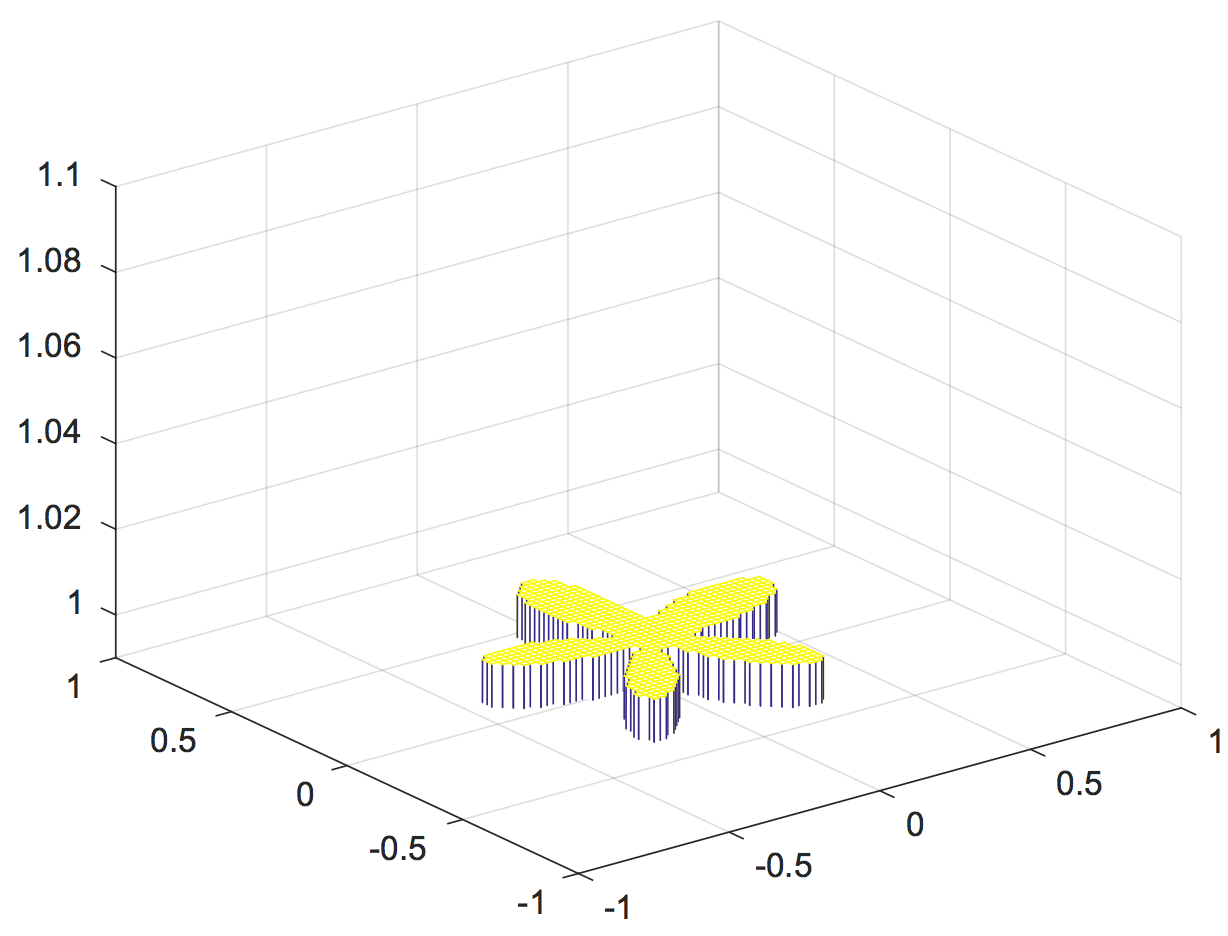
\includegraphics[width=.42\textwidth]{/Users/meganchang/Desktop/Thesis/images/Level_Set_2.png}} \\
\subfigure[$\phi$]{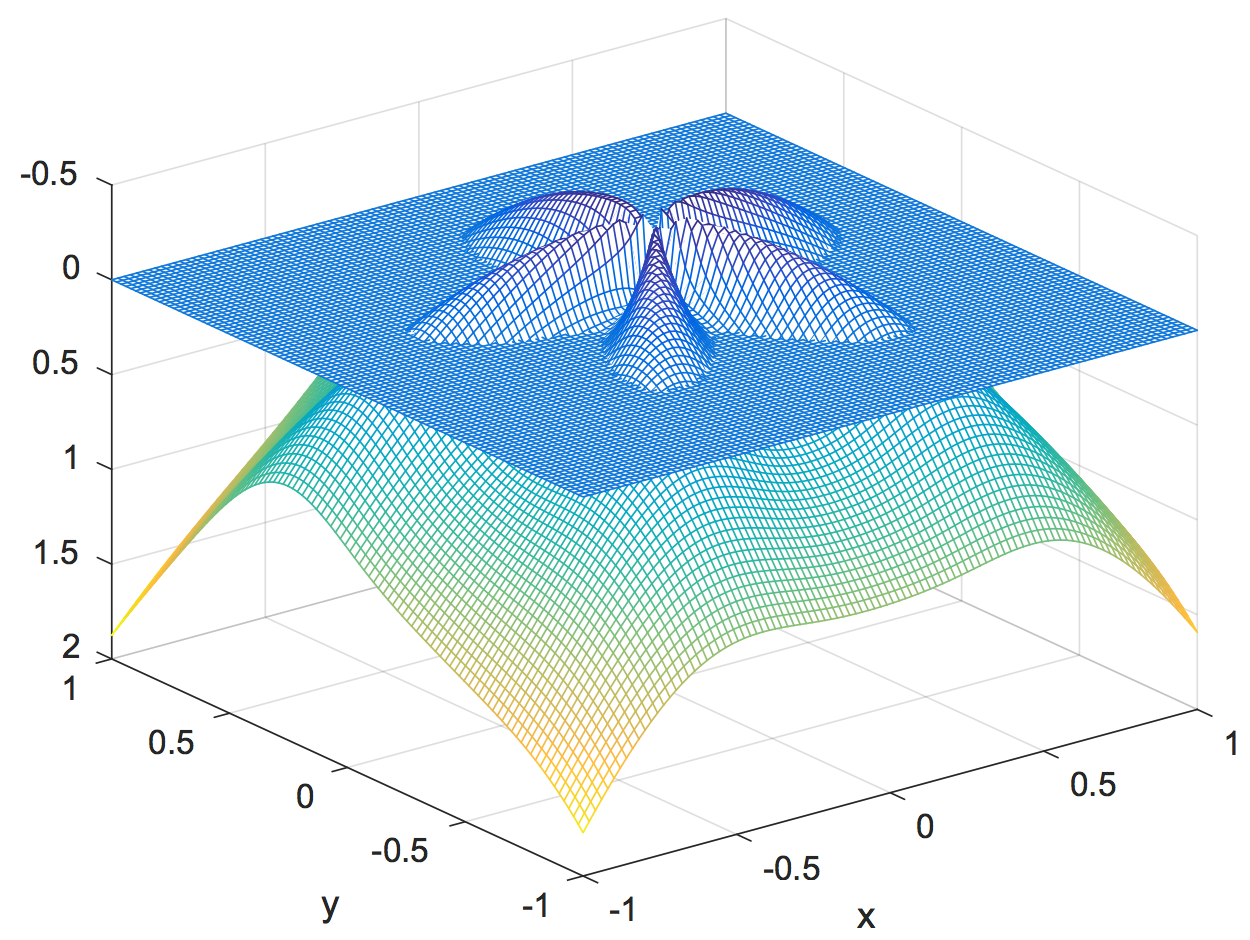
\includegraphics[width=.42\textwidth]{/Users/meganchang/Desktop/Thesis/images/Level_Set_3.png}} \quad
\subfigure[$\Omega^-$]{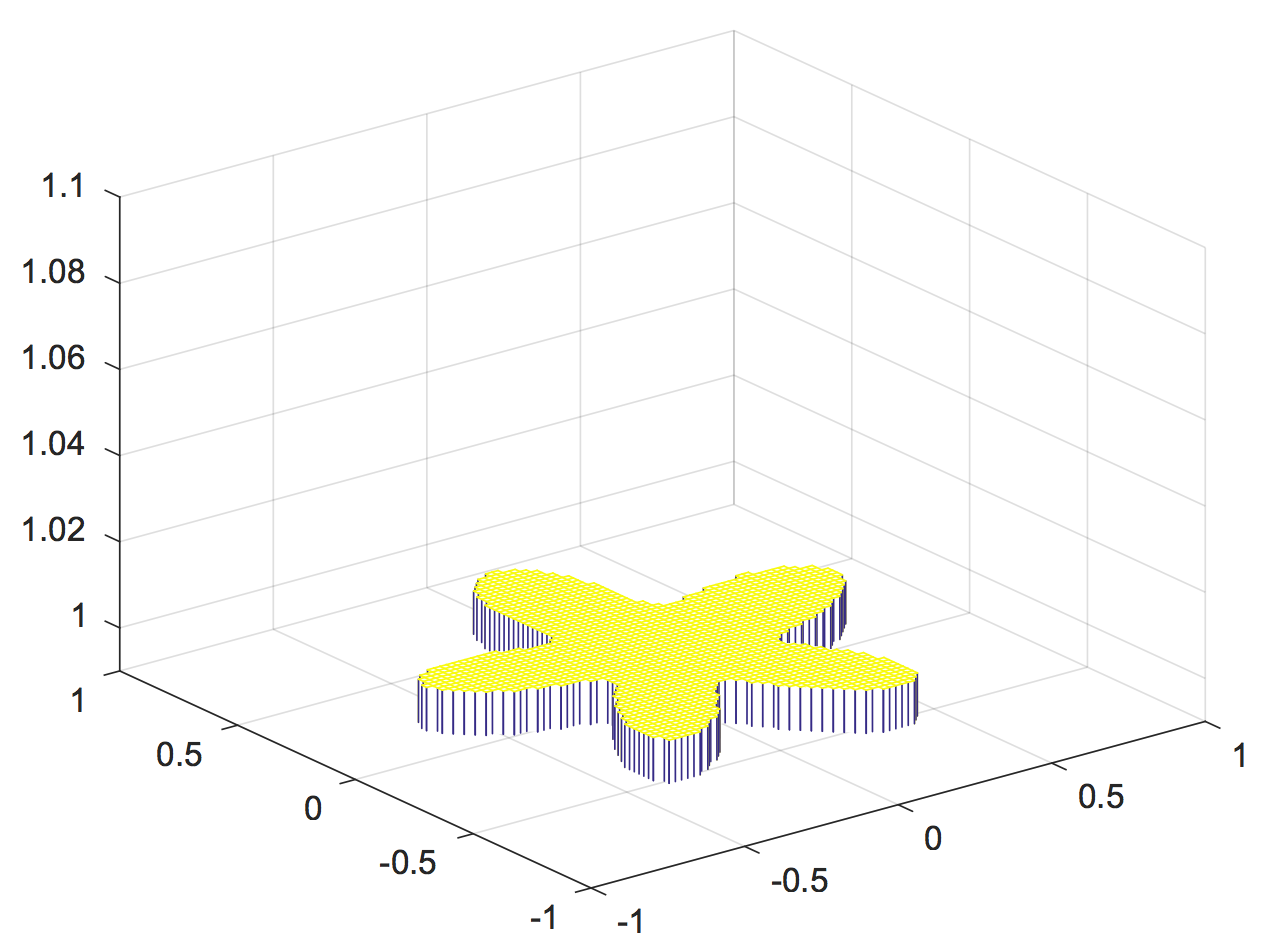
\includegraphics[width=.42\textwidth]{/Users/meganchang/Desktop/Thesis/images/Level_Set_4.png}}\\
\subfigure[$\phi$]{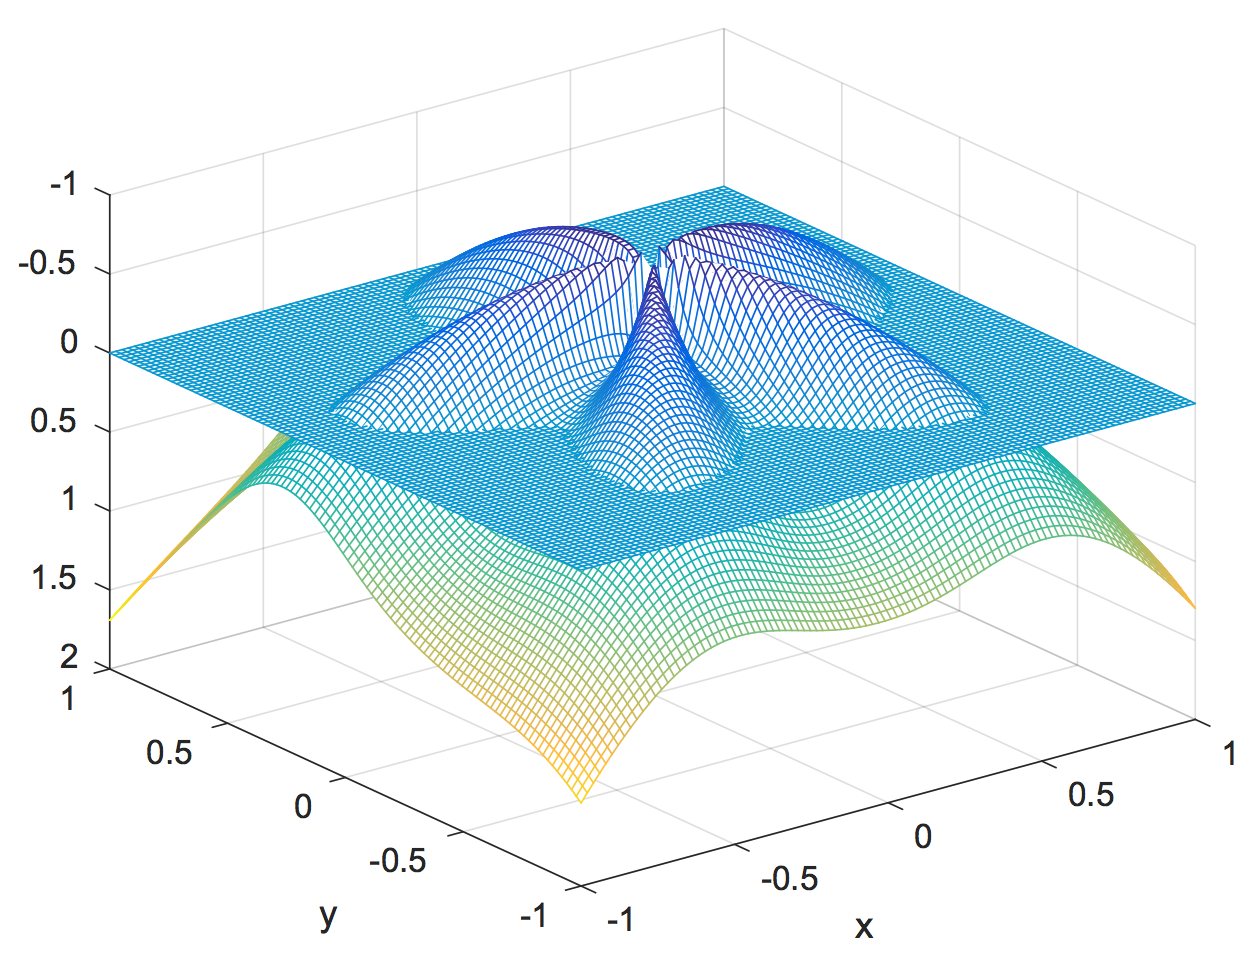
\includegraphics[width=.42\textwidth]{/Users/meganchang/Desktop/Thesis/images/Level_Set_5.png}} \quad
\subfigure[$\Omega^-$]{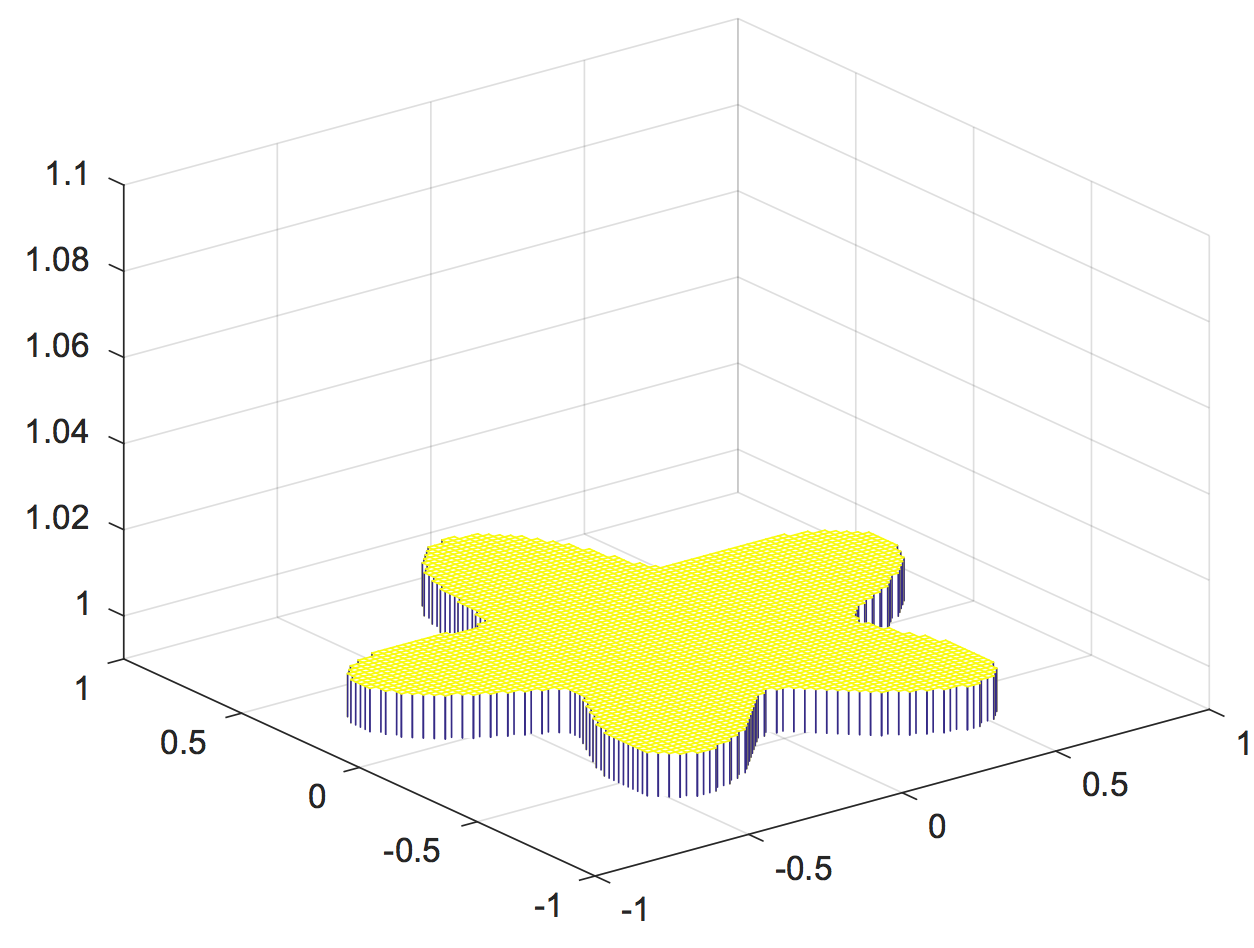
\includegraphics[width=.42\textwidth]{/Users/meganchang/Desktop/Thesis/images/Level_Set_6.png}}
\caption[Interface as an Isocontour of a Higher-Order Dimensional Level-Set Function]{In this example, we use the level-set method to model a flower shape growing uniformly in time. One can see how the negative $\phi$ values in the three-dimensional object on the left create our two-dimensional shape of reacted material on the right, bounded by a border where $\phi = 0$. (The $z$-axis is inverted so that the positive axis points downward.)}
\label{fig:level_set_1}
\end{figure}

\begin{figure} [!h]
\centering
\subfigure[$\phi$]{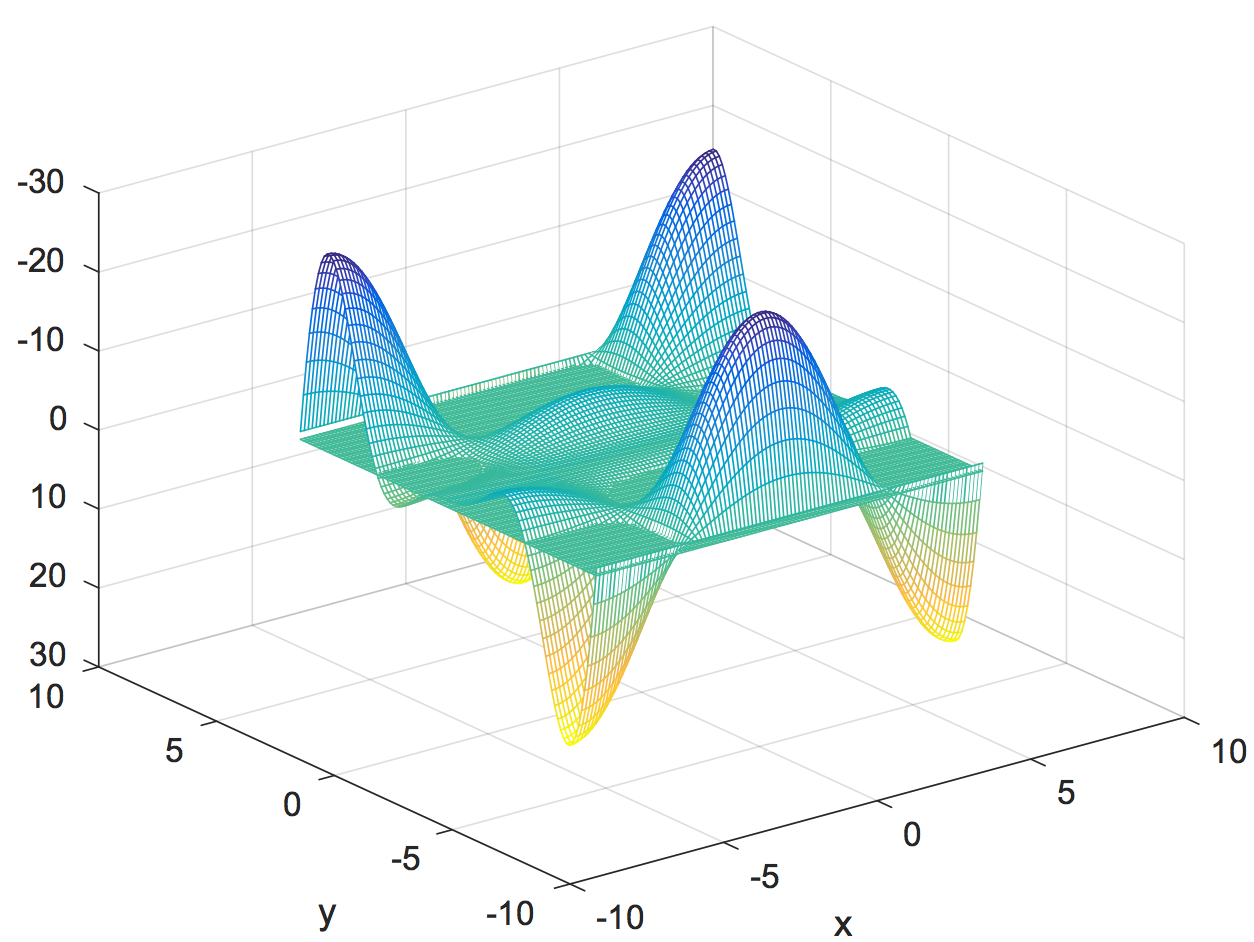
\includegraphics[width=.42\textwidth]{/Users/meganchang/Desktop/Thesis/images/Level_Set_07.png}} \quad
\subfigure[$\Omega^-$]{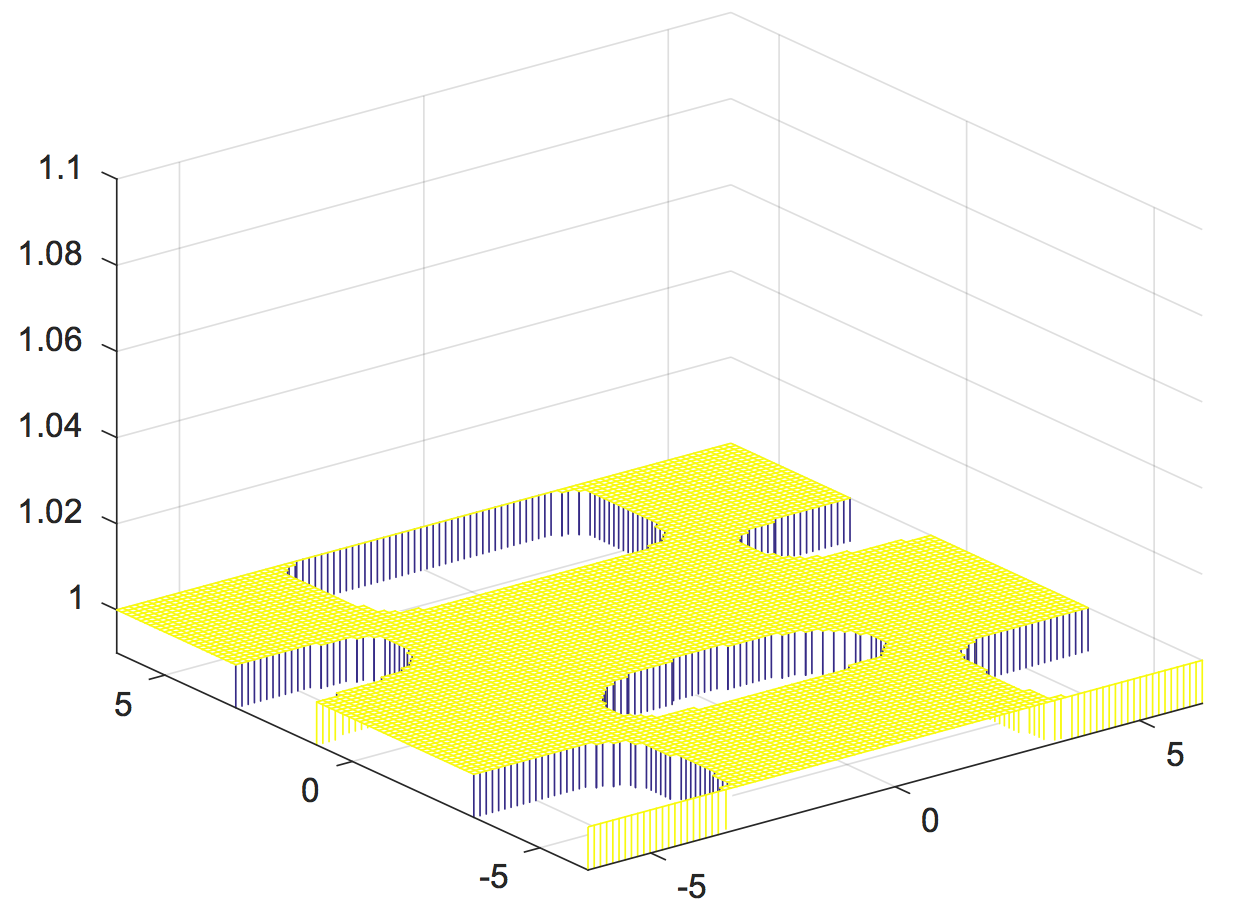
\includegraphics[width=.42\textwidth]{/Users/meganchang/Desktop/Thesis/images/Level_Set_08.png}} \\
\subfigure[$\phi$]{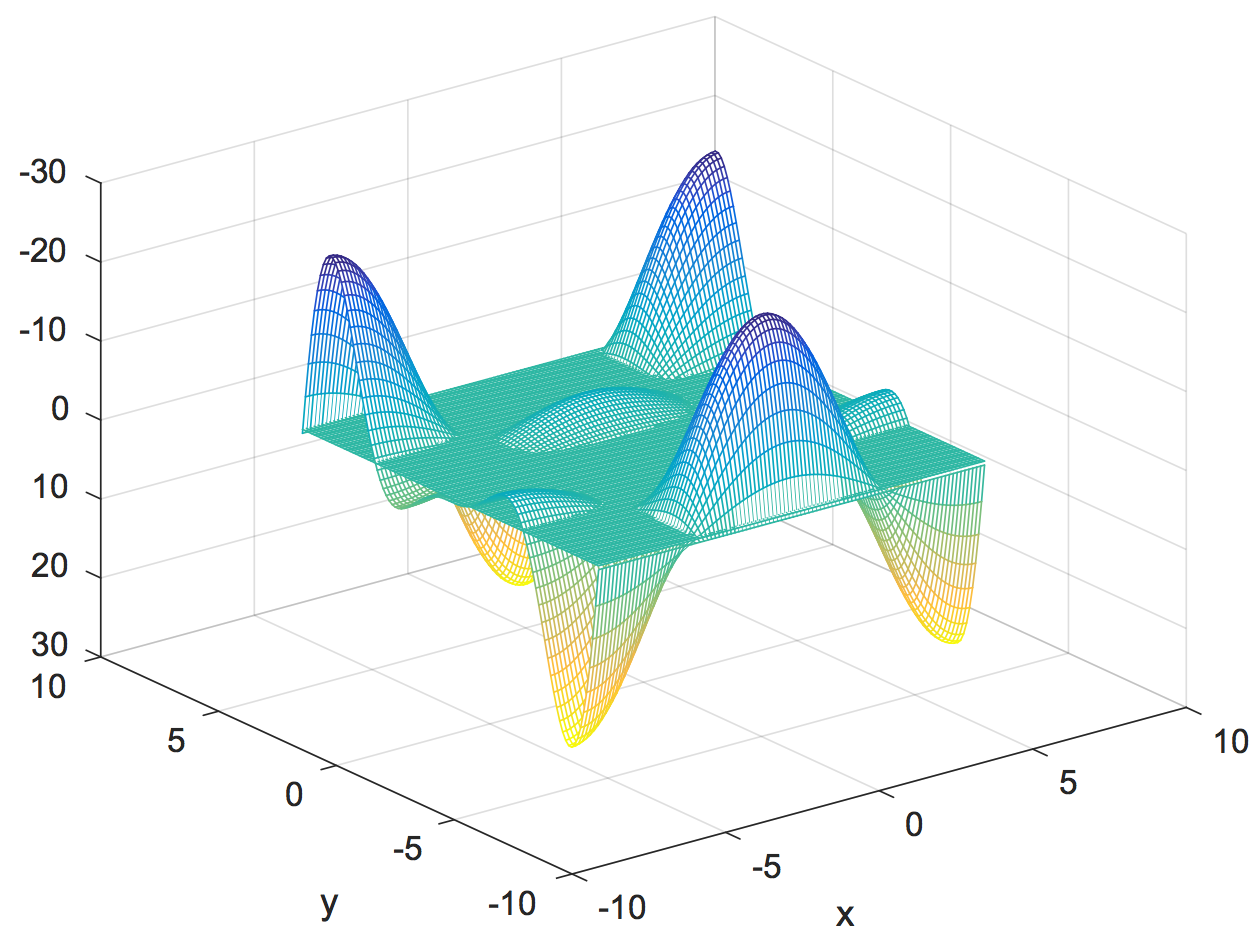
\includegraphics[width=.42\textwidth]{/Users/meganchang/Desktop/Thesis/images/Level_Set_05.png}} \quad
\subfigure[$\Omega^-$]{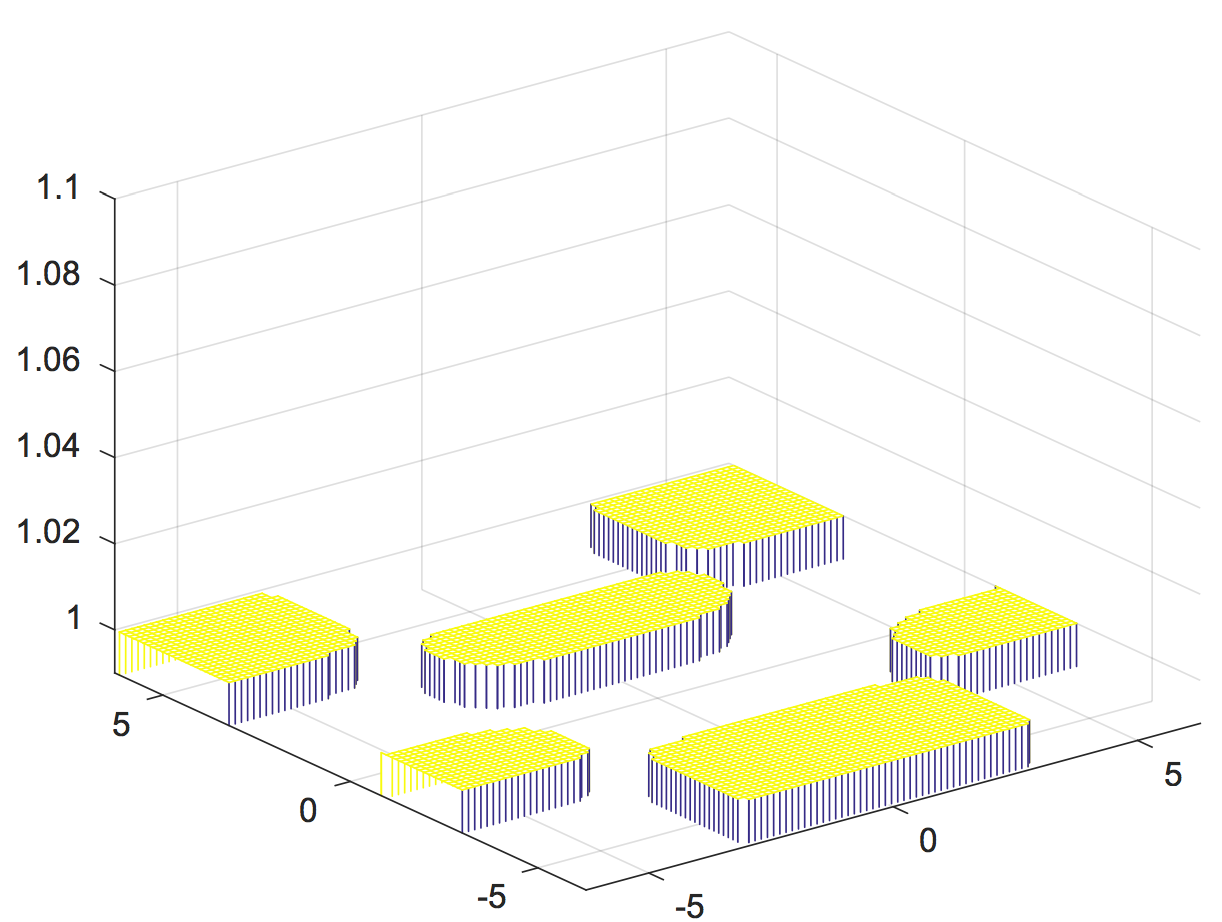
\includegraphics[width=.42\textwidth]{/Users/meganchang/Desktop/Thesis/images/Level_Set_06.png}}\\
\subfigure[$\phi$]{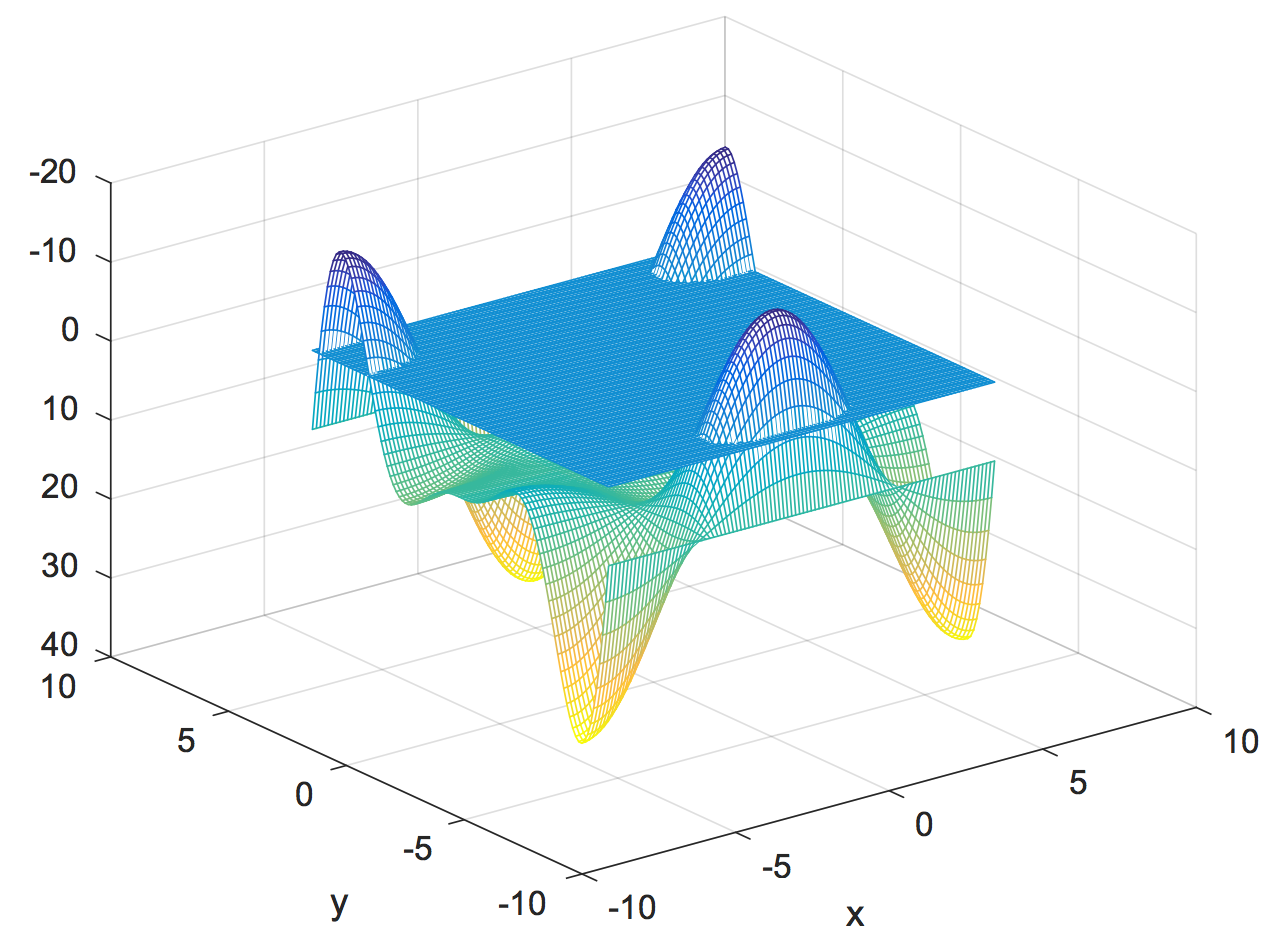
\includegraphics[width=.42\textwidth]{/Users/meganchang/Desktop/Thesis/images/Level_Set_03.png}} \quad
\subfigure[$\Omega^-$]{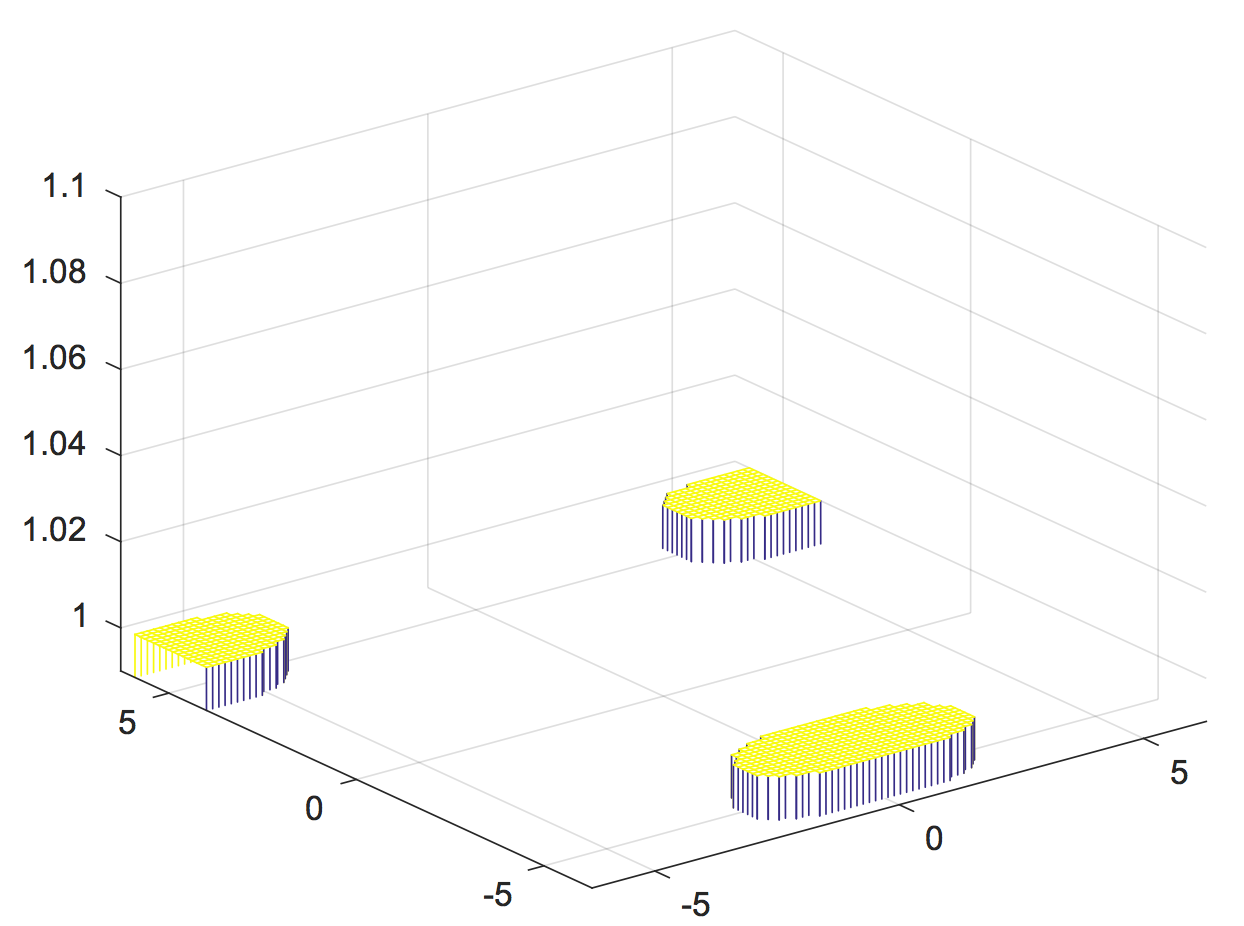
\includegraphics[width=.42\textwidth]{/Users/meganchang/Desktop/Thesis/images/Level_Set_04.png}}
\caption[Level-Set Handling Complex Topological Changes]{In this example, we demonstrate a more complex problem in which reacted material shrinks and separates into individual segments of reacted material. Take for instance a glacier melting and separating into smaller chunks of ice. (The $z$-axis is inverted so that the positive axis points downward.)\\}
\label{fig:level_set_2}
\end{figure}

\section{The Reinitialization Equation} \label{section:Reinitialization_Equation}

The reinitialization scheme, which transforms an arbitrary level-set function into a signed distance function, has been proven to produce more robust numerical results, improve mass conservation, and improve proficiency of geometrical computations such as calculating interface curvatures. When we reinitialize our level-set, we effectively smooth out the gradient and remove any numerical noise that may build up as a result of our moving boundary. Even a small amount of noise will be greatly amplified when calculating the level-set gradients for our normal vectors. This was one of the reasons the level-set method previously had poor mass conservation properties. With the reinitialization method, we greatly reduce this problem.

The reinitialization equation reads
\begin{equation}  
\begin{aligned}
\phi_\tau + S(\phi^0)(|\nabla \phi|-1) = 0
\end{aligned}
\end{equation}
proposed by Sussman, Smereka and Osher in [4], where $S(\phi^0)$ is a smoothed out sign function, and $\tau$ is a fictitious time which allows us to find a steady state solution for $\phi$ with a smooth gradient of magnitude 1, everywhere, while maintaining the location of the zero level-set. In semi-discretized form, this equation can be represented as
\begin{equation} \label{eqn:semi_discretized_reinit}  
\begin{aligned}
\frac{\partial \phi}{\partial \tau} + \text{sgn}(\phi ^0)[H_G(D_x^+ \phi,D_x^- \phi,D_y^+ \phi,D_y^- \phi)-1] = 0,
\end{aligned}
\end{equation}
where $\phi^0$ is the initial level-set at time $\tau = 0$ and sgn$(\phi^0)$ will have a value of either -1 or +1, as determined by the sign of $\phi^0$. Finally, $H_G$ is the Godunov Hamiltonian defined as
\begin{equation}  
    H_G(a,b,c,d) = 
\begin{cases}
    \sqrt{\text{max}(|a^+|^2,|b^-|^2) + \text{max}(|c^+|^2,|d^-|^2)}& \text{if sgn}(\phi^0) < 0,  \\  \sqrt{\text{max}(|a^-|^2,|b^+|^2) + \text{max}(|c^-|^2,|d^+|^2)} & \text{if sgn}(\phi^0) > 0,
\end{cases}
\end{equation}
where $a^+ =$ max$(a,0)$ and $a^- =$ min$(a,0)$. Further, from \eqref{eqn:semi_discretized_reinit}, we know that $a$, $b$, $c$, and $d$ correspond to the directional derivatives $D_x^+ \phi,D_x^- \phi,D_y^+ \phi$, and $D_y^- \phi$ computed using first-order accurate one-sided finite differences
\begin{equation} \label{eqn:directional_derivatives}
\begin{aligned}
D_x^+ \phi_{i,j} = \frac{\phi_{i+1,j}-\phi_{i,j}}{\Delta x},\\
D_x^- \phi_{i,j} = \frac{\phi_{i,j}-\phi_{i-1,j}}{\Delta x},\\
D_y^+ \phi_{i,j} = \frac{\phi_{i,j+1}-\phi_{i,j}}{\Delta y},\\
D_y^- \phi_{i,j} = \frac{\phi_{i,j}-\phi_{i,j-1}}{\Delta y},
\end{aligned}
\end{equation}
where in derivative notation, the subscript denotes a partial derivative with respect to either $x$ or $y$, and the superscript denotes the upwind direction (either + or -) to indicate whether the points $i$ and $i+1$ are involved, or $i$ and $i-1$, respectively.

Next, we evolve our solution in time using the second-order accurate Total Variation Diminishing Runge-Kutta (TVD RK2) scheme which uses two Euler steps to develop a temporary $\tilde{\phi}^{n+2}$ value
\begin{equation} \label{eqn:TVD_RK-2}
\begin{aligned}
\frac{\tilde{\phi}^{n+1} - \phi^n}{\Delta \tau} &+ \text{sgn}(\phi ^0)[H_G(D_x^+ \phi^n,D_x^- \phi^n,D_y^+ \phi^n,D_y^- \phi^n)-1] = 0,\\
\frac{\tilde{\phi}^{n+2} - \tilde{\phi}^{n+1}}{\Delta \tau} &+ \text{sgn}(\phi ^0)[H_G(D_x^+ \tilde{\phi}^{n+1},D_x^- \tilde{\phi}^{n+1},D_y^+ \tilde{\phi}^{n+1},D_y^- \tilde{\phi}^{n+1})-1] = 0,
\end{aligned}
\end{equation}
and one averaging step to achieve a second-order accurate value for $\phi^{n+1}$
\begin{equation}  
\begin{aligned}
\phi^{n+1} = \frac{\phi^n + \tilde{\phi}^{n+2}}{2}.
\end{aligned}
\end{equation}
Again, $\tau$ is a fictitious time which allows us to evolve our solution until steady state is reached by reinserting $\phi^{n+1}$ into the above equations as our new $\phi^n$. For stability purposes, we select a $\Delta \tau = 0.5$ min$(\Delta x, \Delta y)$ for our fictitious time step.

Notice, however, that in \eqref{eqn:TVD_RK-2}, despite the time step $n$, we continue to use the sign of the initial level-set (i.e. sgn$(\phi^0)$). This is because we do not want the interface moving during reinitialization. That is to say, the sign of $\phi_{i,j}$ should be consistent throughout this process in order to preserve area and uphold conservation of mass.

Also to comply with mass conservation, extra care must be taken at the points neighboring the interface [4]. More often than not, the interface will not fall exactly on a grid point $\phi_{i,j}$. So instead of being represented by a zero value, the interface will be located between two grid nodes that are \textbf{changing sign}, such that $\phi_{i,j} \cdot \phi_{i-1,j} < 0$. For these points, it is necessary to calculate the value $\theta$ which represents the fractional distance between the interface and the neighboring grid points. We calculate these $\theta$ values before entering our iterative solver since this distance $\theta$ should remain constant throughout the reinitialization process. These $\theta$ values can then be used to maintain the zero level-set and ensure the location of our interface does not change during reinitialization. So, assuming that our point of interest $\phi_{i,j} < 0$, we would then calculate $\theta$ as 
\begin{equation}\label{eqn:theta^L}
\theta_{i,j}^L = \frac{\phi_{i,j}}{\phi_{i,j}-\phi_{i-1,j}} \quad \quad \text{if $\phi_{i,j} \cdot \phi_{i-1,j} < 0$}, \\
\end{equation}
where the superscript $L$ indicates that the interface passes to the left of the point $\phi_{i,j}$. Note, for each grid point, there can be up to four values of $\theta$ associated to it since it is possible for the interface to pass a point on more than one side. For instance, if the interface passed to the left and above it, our point $\phi_{i,j}$ would have a $\theta^L_{i,j}$ and $\theta^A_{i,j}$ associated to it. The other three possible $\theta$ values for a point $\phi_{i,j}$ are calculated as
\begin{equation}\label{eqn:thetas}
\begin{aligned}
    \theta_{i,j}^R = \frac{\phi_{i,j}}{\phi_{i,j}-\phi_{i+1,j}} & \quad \quad \text{if $\phi_{i,j} \cdot \phi_{i+1,j} < 0$}, \\
    \theta_{i,j}^B = \frac{\phi_{i,j}}{\phi_{i,j}-\phi_{i,j-1}} & \quad  \quad  \text{if $\phi_{i,j} \cdot \phi_{i,j-1} < 0$}, \\
    \theta_{i,j}^A = \frac{\phi_{i,j}}{\phi_{i,j}-\phi_{i,j+1}} &  \quad \quad \text{if $\phi_{i,j} \cdot \phi_{i,j+1} < 0$},
\end{aligned}
\end{equation}
where $\theta$ must always be positive. These $\theta$ values are then used to recompute the directional derivatives at that point $\phi_{i,j}$
\begin{equation}
\begin{aligned}
D_x^+ \phi_{i,j} = \frac{\phi_{I,j}-\phi_{i,j}}{\theta^R_{i,j} \Delta x},\\
D_x^- \phi_{i,j} = \frac{\phi_{i,j}-\phi_{I,j}}{\theta^L_{i,j} \Delta x},
\end{aligned}
\end{equation}
where $\phi_{I,j}$ is the value of $\phi$ at the interface, and since we know this to be zero, these equations can simply be written as
\begin{equation}
\begin{aligned}
D_x^+ \phi_{i,j} = \frac{-\phi_{i,j}}{\theta^R_{i,j} \Delta x},\\
D_x^- \phi_{i,j} = \frac{\phi_{i,j}}{\theta^L_{i,j} \Delta x},
\end{aligned}
\end{equation}
with similar construction for the directional derivatives with respect to $y$:
\begin{equation}
\begin{aligned}
D_y^+ \phi_{i,j} = \frac{-\phi_{i,j}}{\theta^A_{i,j} \Delta y},\\
D_y^- \phi_{i,j} = \frac{\phi_{i,j}}{\theta^B_{i,j} \Delta y}.
\end{aligned}
\end{equation}
For these points $\phi_{i,j}$ that have at least one associated $\theta$ value, a new time step stability restriction must be satisfied:
\begin{equation}
\Delta \tau = 0.5\text{min}(\theta^R \Delta x, \theta^L \Delta x, \theta^A \Delta y, \theta^B \Delta y).
\end{equation}
Also, notice that $\theta$ is in the denominator of our one-sided finite difference calculations. This means small values of $\theta$ can cause numerical instabilities. To avoid producing non-finite data, we say that if $\theta$ is too small ($\theta < \Delta x$), we can assume the point is very close to the interface, and set $\phi_{i,j} = 0$, reassigning this point to the interface. This small perturbation in the location of the zero level-set (also known as artificial boundary perturbation) has a negligible impact on the accuracy of our solver, and guarantees numerical stability. Figure \ref{fig:reinitialization_1} shows how effectively the zero level-set is maintained on a complex geometry with sharp kinks.
\begin{figure} [!h]
\centering
\subfigure[Zero level-set contour]{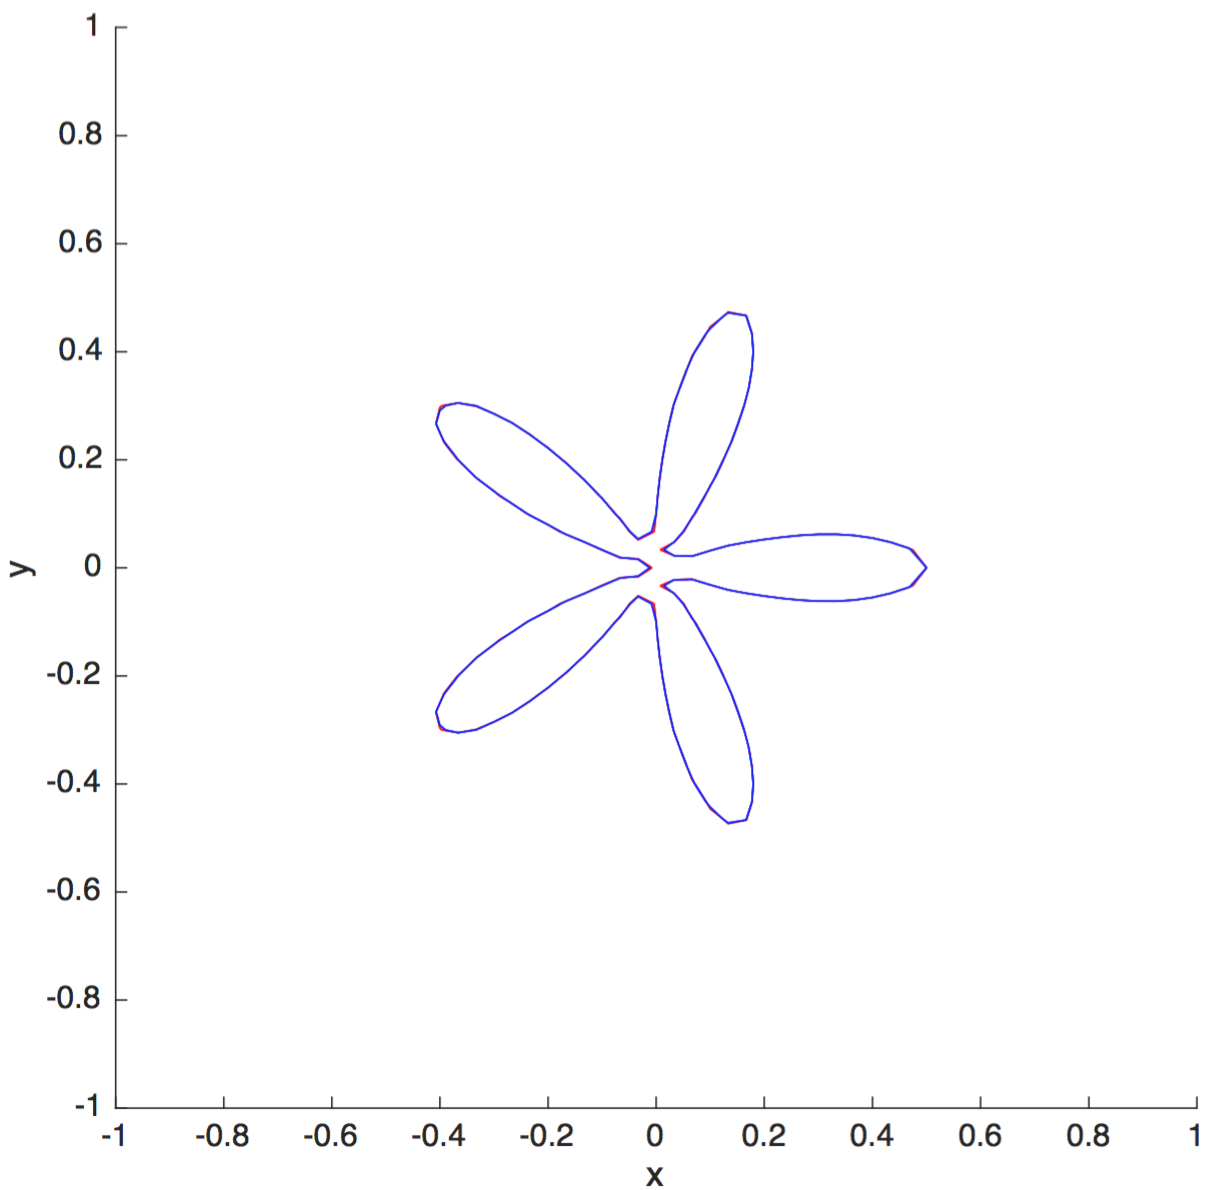
\includegraphics[width=.48\textwidth]{/Users/meganchang/Desktop/Thesis/images/Reinitialize_zero_level_set_1.png}} \quad
\subfigure[Zoomed in]{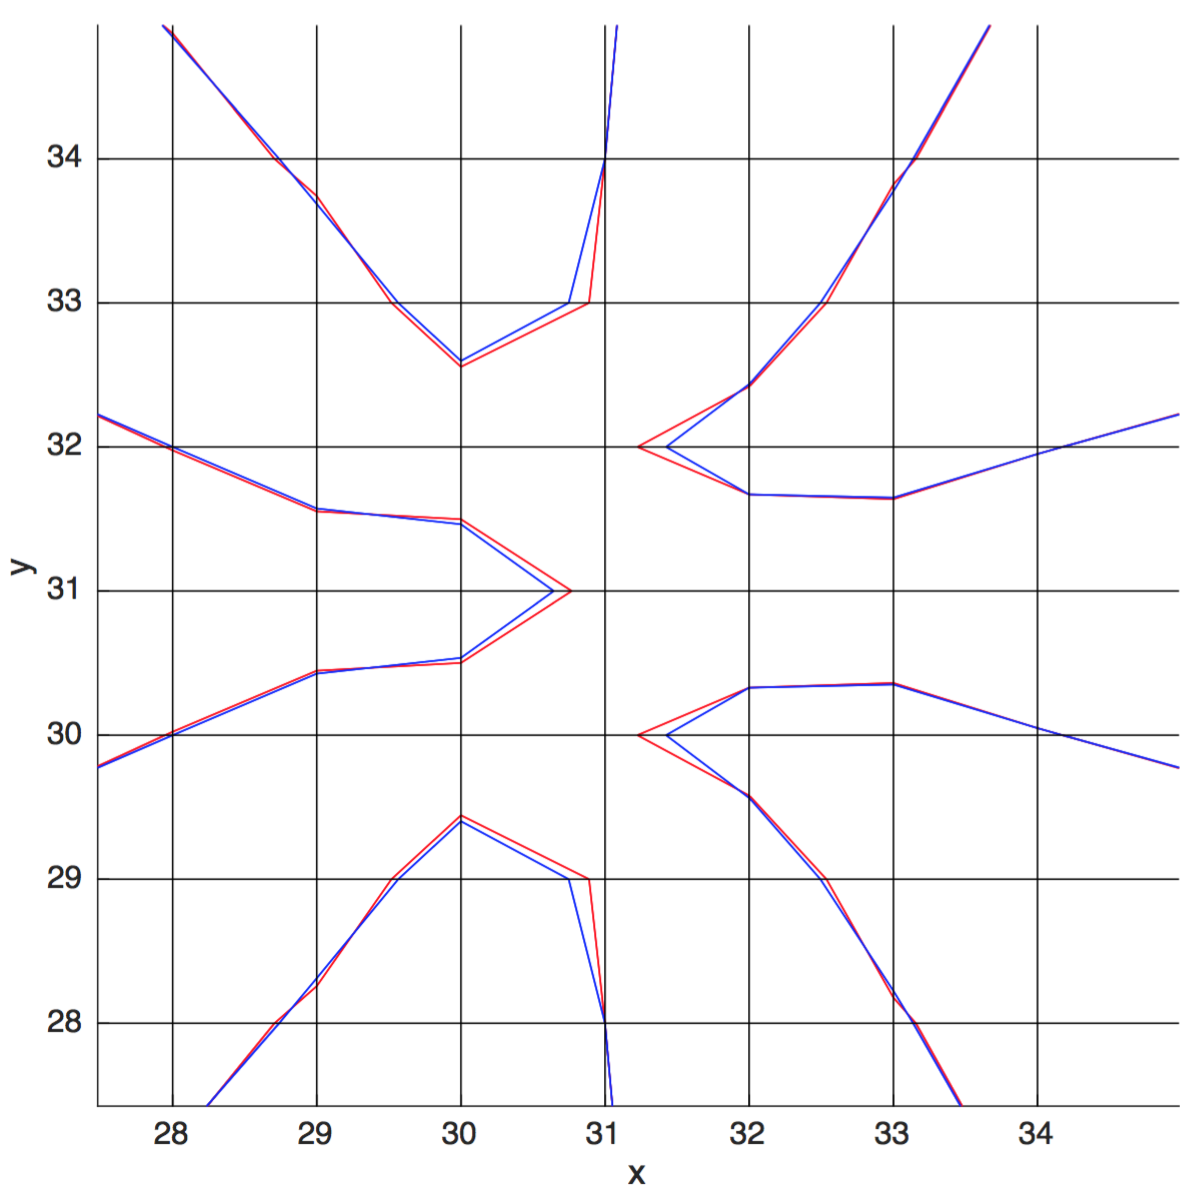
\includegraphics[width=.48\textwidth]{/Users/meganchang/Desktop/Thesis/images/Reinitialize_zero_level_set_2.png}} \\
  \caption[Maintaining the Zero Level-Set During Reinitialization]{The zero level-set is effectively maintained throughout the reinitizialization scheme. The red line shows the original zero level-set location, while the blue is the new zero level-set location after the function has been reinitialized. The goal is for the blue to completely overlap the red one. In (b), we have zoomed into an area with sharp kinks and where some points have more than one $\theta$ value. This is where problems would arise, but our scheme is able to maintain $\phi_0^0$ nicely.}
  \label{fig:reinitialization_1}
\end{figure}
And Figure \ref{fig:reinitialization_2} best demonstrates visually what is achieved via the reinitialization method, where one will notice our original level-set shaped as a bowl is reinitialized into a cone-like shape. Also notice that the initial level-set is very noisy (i.e. the data does not appear smooth). This noise is removed via reinitialization so that it does not create large numerical errors when calculating $\nabla \phi$. It is important to note that beyond interface tracking, $\phi$ has no relevant meaning. This means we care only about the zero level-set's position, and the sign of $\phi$ which tells us which material region we are in (either $\Omega^-$ or $\Omega^+)$. The actual magnitude of $\phi$, however, is irrelevant.
\begin{figure} [!h]
\centering
\subfigure[Before]{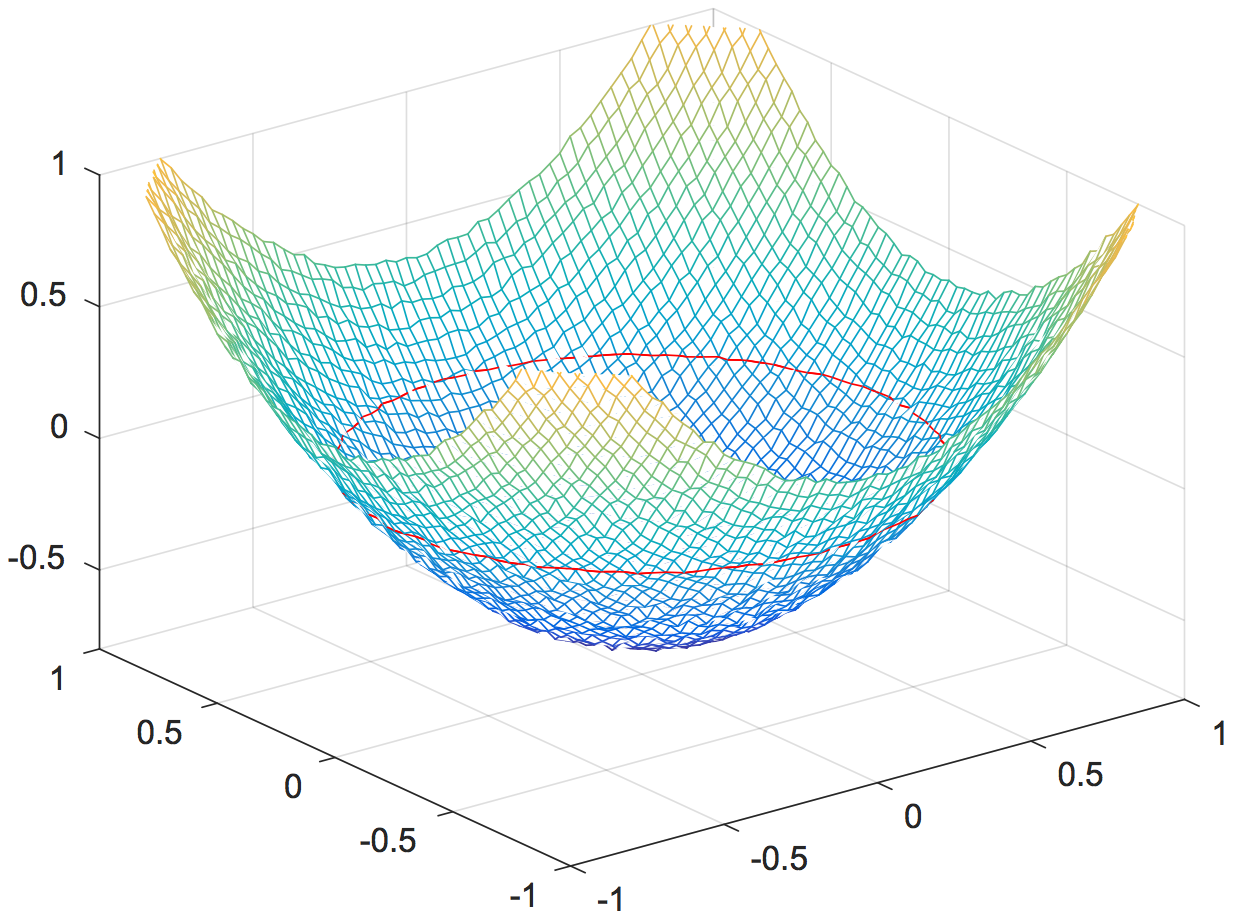
\includegraphics[width=.48\textwidth]{/Users/meganchang/Desktop/Thesis/images/Noisy_1.png}} \quad
\subfigure[After]{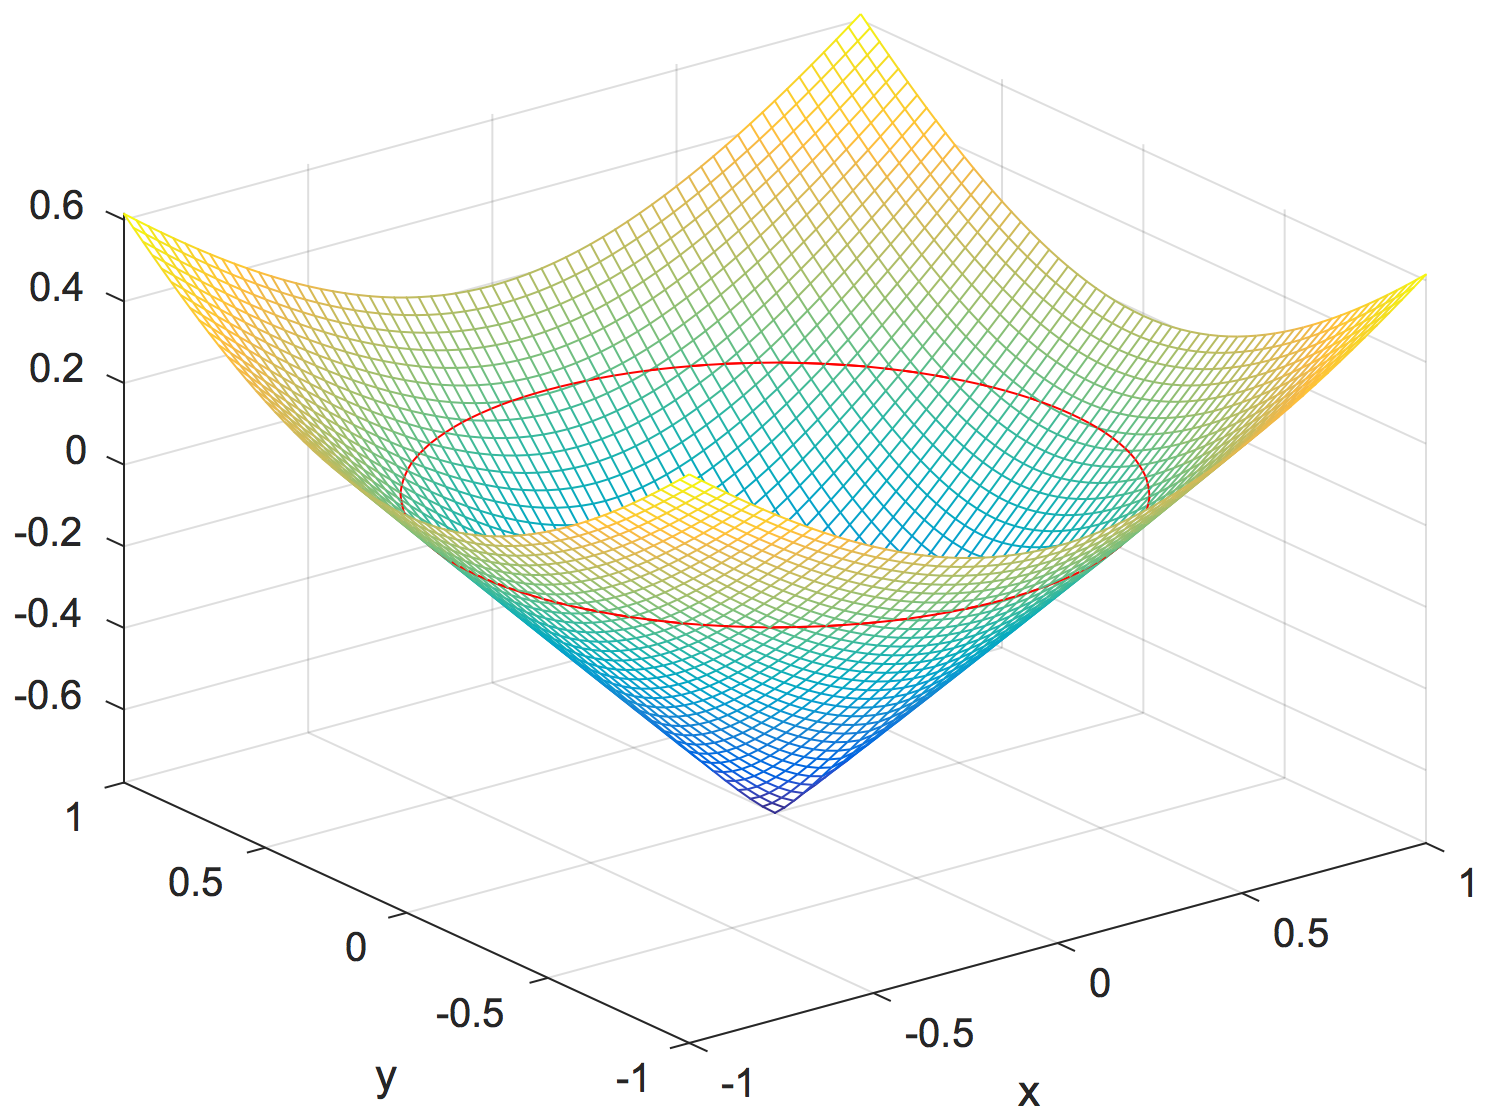
\includegraphics[width=.48\textwidth]{/Users/meganchang/Desktop/Thesis/images/Reinitialize_After_1.png}}
  \caption[Reinitializing the Level-Set]{The reinitialization scheme will take a noisy level-set and return as an output, a level-set with a smooth gradient of magnitude 1, everywhere. This makes them produce more robust numerical results, especially when computing normal vectors which rely on $\phi$ gradients. The red isocontour line represents the zero level-set, which has not moved during the reinitialization process.}
  \label{fig:reinitialization_2}
\end{figure}

%=== Chapter 3  ============================================
\chapter{Diffusion}\label{section:Diffusion}

Diffusion describes the net movement of particles from a region of high concentration to a region of lower concentration due to molecular Brownian motion. For example, consider a drop of colored ink in a glass of water. Assume we are dealing with an ink droplet with the same density as water that has been placed in a state of suspension, completely undisturbed by convection or gravitational effects. With time, the ink would naturally spread, so that eventually the cup of water would be uniformly colored with uniform distribution of the ink concentration. This natural phenomenon of homogenization is described by
\begin{equation}\label{eqn:diffusion}
\frac{\partial u}{\partial t} = \nabla \cdot (D \nabla u) + S,
\end{equation}
where $u$ is the concentration, $D$ is the diffusion coefficient, and $S$ is the source term. We use the implicit Crank-Nicholson scheme in semi-discretized form
\begin{equation}\label{eqn:Crank}
\frac{u^{n+1}-u^n}{\Delta t} = \frac{1}{2}\nabla \cdot (D \nabla u^{n+1}) + \frac{1}{2}\nabla \cdot (D \nabla u^{n}) + \frac{1}{2}(S^{n+1}+S^{n}),
\end{equation}
because it allows us to achieve second-order accuracy in space and time using $\Delta t \sim \Delta x$. This way, as we refine our grid, our time step gets proportionally smaller, rather than quadratically smaller. Further, we know our time step will be limited by advection, rather than diffusion to ensure stability. In discretized form, for a two-dimensional problem with constant $D$ and standard centered finite differences in space, we obtain
\begin{equation}
\begin{aligned}
\frac{u_{i,j}^{n+1} - u_{i,j}^{n}}{\Delta t} &= \frac{1}{2}D  \bigg(\frac{u_{i-1,j}^{n+1} - 2u_{i,j}^{n+1} +  u_{i+1,j}^{n+1}}{\Delta x^2} + \frac{u_{i,j-1}^{n+1} - 2u_{i,j}^{n+1} + u_{i,j+1}^{n+1}}{\Delta y^2}\\
\>\>\>+ 
&\frac{u_{i-1,j}^{n} - 2u_{i,j}^{n} + u_{i+1,j}^{n}}{\Delta x^2} + \frac{u_{i,j-1}^{n} - 2u_{i,j}^{n} + u_{i,j+1}^{n}}{\Delta y^2}\bigg)
+ \frac{1}{2}(S_{i,j}^{n+1} + S_{i,j}^{n}).
\end{aligned}
\end{equation}
And if we rearrange our system of linear equations to resemble $\boldsymbol{A}\vec{u}^{\>n+1} = \vec{f}\>(\vec{u}^{\>n},BC^{n+1})$, so that all our knowns are on the RHS, we are left with
\begin{equation}\label{eqn:Crank_discretized}
\begin{aligned}
&\frac{u_{i,j}^{n+1}}{\Delta t} - \frac{1}{2}D \bigg(\frac{u_{i-1,j}^{n+1}- 2u_{i,j}^{n+1} + u_{i+1,j}^{n+1}}{\Delta x^2} + \frac{u_{i,j-1}^{n+1} - 2u_{i,j}^{n+1} + u_{i,j+1}^{n+1}}{\Delta y^2}\bigg)\\
&= \frac{u_{i,j}^{n}}{\Delta t} + \frac{1}{2}D\bigg(\frac{{u_{i-1,j}^{n}} - 2u_{i,j}^{n} + u_{i+1,j}^{n}}{\Delta x^2} + \frac{u_{i,j-1}^{n} - 2u_{i,j}^{n} + {u_{i,j+1}^{n}}}{\Delta y^2}\bigg)
+ \frac{1}{2}(S_{i,j}^{n+1} + S_{i,j}^{n}),
\end{aligned}
\end{equation}
where $\boldsymbol{A}$ is our diffusion matrix and  $\vec{u}^{\>n+1}$ is our vector of unknowns at the next time step assuming that our source term does not depend on $u$.

\section{Building an Efficient Sparse Matrix}\label{section:Sparse_Matrix}

Since our matrix will contain mostly zero elements, we can significantly minimize memory usage by creating a sparse matrix $\boldsymbol{A}$. So, rather than populate a full matrix with a few non-zero elements $A_{i,j}$, we simply keep track of the non-zero $\boldsymbol{A}$ element's value and location in three separate vectors: $\vec{A}, \vec{i},$ and $\vec{j}$. Then, we use Matlab's built-in sparse function to generate a sparse matrix. For example, the following matrix

\dhalfsp
\begin{equation*}
A = 
\begin{bmatrix}
15 & 0 & 0 & 0\\
0 & 25 & 0 & 0\\
0 & 17 & 35 & 0\\
0 & 0 & 0 & 45
\end{bmatrix}
\end{equation*}
would instead be represented as
\begin{equation*}
\begin{aligned}
\vec{A} =&
\begin{bmatrix}
15 & 25 & 17 & 35 & 45
\end{bmatrix},\\
\vec{i} \>=&
\begin{bmatrix}
\> 1 &\>\> 2 &\>\>\> 3 &\>\> 3 &\>\> 4 \>\>
\end{bmatrix},\\
\vec{j} \>=&
\begin{bmatrix}
\> 1 &\>\> 2 &\>\> 2 & \>\>\>3 &\>\> 4 \>\>
\end{bmatrix},
\end{aligned}
\end{equation*}
\dsp
where $\vec{A}$ contains the values of the non-zero elements, and $\vec{i}$ and $\vec{j}$ contain their row and column locations. While this may not appear useful for a 4$\times$4 matrix, the sparse indexing method becomes highly advantageous as $\boldsymbol{A}$ grows. Take, for example, an identity matrix of size 1,000$\times$1,000. In full matrix storage mode, this matrix requires 8 megabytes of memory. In sparse mode, it requires only 0.024 megabytes (that equates to a 99.7\% reduction in memory space). Since each row of our matrix can have at most five non-zero elements regardless of the grid resolution, the sparse matrix is highly effective for our purposes.

This greatly reduces memory usage, but requires some additional preparation. In order to preallocate the size of our RHS vector, we count the number of points contained in $\Omega^-$. To preallocate the size of our sparse vectors $\vec{A}, \vec{i},$ and $\vec{j}$, we must count all of the points in  $\Omega^-$, and additionally count the nupmber of neighbors also encompassed within $\Omega^-$ using the product test (e.g. $\phi_{i,j}^{n+1} \cdot \phi_{i+1,j}^{n+1} > 0$).

\clearpage
Now, we are ready to fill our sparse vector $\vec{A}$. We take the coefficients directly from the discretized diffusion equation \eqref{eqn:Crank_discretized}:
\dhalfsp
\begin{equation*}
\text{Above} =-\frac{1}{2}D\frac{\Delta t}{\Delta y^2},
\end{equation*}
\begin{equation*}
\text{Left}  =-\frac{1}{2}D\frac{\Delta t}{\Delta x^2}, \quad \quad \quad \text{Center} = 1 + \frac{1}{2}D\bigg(\frac{2 \Delta t}{\Delta x^2} + \frac{2 \Delta t}{\Delta y^2}\bigg), \quad \quad  \quad \text{Right} =-\frac{1}{2}D\frac{\Delta t}{\Delta x^2},
\end{equation*}
\begin{equation}\label{eqn:Crank_coeffs}
\text{Below} =-\frac{1}{2}D\frac{\Delta t}{\Delta y^2}.
\end{equation}

\dsp
Each time we add a value to $\vec{A}$, we also add its position to our $\vec{i}$ and $\vec{j}$ vectors. For instance, for a point $\phi_{i,j}^{n+1}$ contained in $\Omega^-$, we add five elements to each of our vectors ($\vec{A}$, $\vec{i}$, and $\vec{j}$) as shown in Table \ref{table:Sparse_Vectors}. To understand this table, we must introduce two new functions: the column-stacking function $p$ and the tagging function.

Our system of linear equations $\boldsymbol{A}\vec{u}^{\>n+1} = \vec{f}\>(\vec{u}^{\>n},BC^{n+1})$ requires $u$ to be stored in vector form. Thus, we store our elements of $u_{i,j}^{n+1}$ in a vector $\vec{u}_p^ \> {n+1}$, where

\begin{equation}
p  = (j-1)m+i.
\end{equation}
This function allows us to stack our $u_{i,j}$ values, column by column, where $m$ corresponds to the number of elements in a column for an $m$$\times$$n$ grid, $i$ and $j$ correspond to the location of $u_{i,j}$ in the grid, and $p$ is a number from 1 to $m\cdot n$ corresponding to the index of $u$ in the vector $\vec{u}_p^ \> {n+1}$.

Further, we must define our tag function, a system which was implemented in order to remove any trivial equations such as discretizations at grid points outside of $\Omega^-$, where the solution was invalid and unused (i.e. $u^{n+1}_{p} = 0$). Skipping the creation of these trivial equations greatly improved computational efficiency, but changed the location of points in our vector $\vec{u}_p^ \> {n+1}$. Consider, for example, if the first linear equation were to be removed. Every element in the vector $\vec{u}_p^ \> {n+1}$ would now be located at $p-1$ (e.g. $u_{2}^{n+1}$ would now be $u_{1}^{n+1}$). This tagging system filters through each grid point and \textit{tags} any nontrivial points so that we can properly locate them in our nontrivial vector $\vec{u}_p^ \> {n+1}$.

\begin{table} [ht]
\caption{Sparse Matrix Location Vectors}\label{table:Sparse_Vectors}
\centering
\begin{tabular}{c c c}
\hline
$\vec{A}$ & $\vec{i}$ & $\vec{j}$\\ \hline
Center   & $\text{tag}(p(i,j,m))$        &  $\text{tag}(p(i,j,m))$     \\
Left        & $\text{tag}(p(i-1,j,m))$    &  $\text{tag}(p(i,j,m))$     \\
Right     & $\text{tag}(p(i+1,j,m))$    &  $\text{tag}(p(i,j,m))$     \\
Below    & $\text{tag}(p(i,j,m))$        &  $\text{tag}(p(i,j-1,m))$   \\
Above    & $\text{tag}(p(i,j,m))$        &  $\text{tag}(p(i,j+1,m))$   \\
\end{tabular}
\end{table}

Table \ref{table:Sparse_Vectors} describes how we would handle a point in which all the neighboring points are also encompassed in the reacted region $\Omega^-$. If this is not the case - that is to say, if a neighboring point was in $\Omega^+$, we would use a different treatment. In this case, we would not include a term in our $\boldsymbol{A}$ matrix. Instead, we must introduce ghost points.

\section{Building a Symmetric Matrix to Treat Diffusion on Irregular Domains (The Ghost Fluid Method)}\label{section:Symmetric_Matrix}

In constructing our diffusion matrix $\boldsymbol{A}\vec{u}^{\>n+1} = \vec{f}\>(\vec{u}^{\>n},BC^{n+1})$, we consider only our unknown values of interest, such that $\vec{u}^{\>n+1}$ contains only values within the $\Omega^-$ domain. To reiterate, we can ignore any points that fall exactly on the interface $\phi_0^{n+1}$, where Dirichlet boundary conditions are given, as well as any points in $\Omega^+$.

Now, consider the example shown in Figure \ref{fig:ghost_node}. Consider a point neighboring the interface such as $u_{2,2}^{n+1}$. To account for diffusion from $u_{2,3}^{n+1}$ and $u_{3,2}^{n+1}$, we implement the process developed in the previous section. However, we know that $u_{2,1}^{n+1} = u_\gamma$ since it falls on the interface, and $u_{1,2}^{n+1}$ is contained in $\Omega^+$. Since both of these points are excluded from our vector $\vec{u}^{\>n+1}$, but are needed in the discretization at $u_{2,2}^{n+1}$, we must define \textbf{ghost nodes} as proposed in [1] by Gibou and Fedkiw.

\begin{figure}[h!]
    \centering
    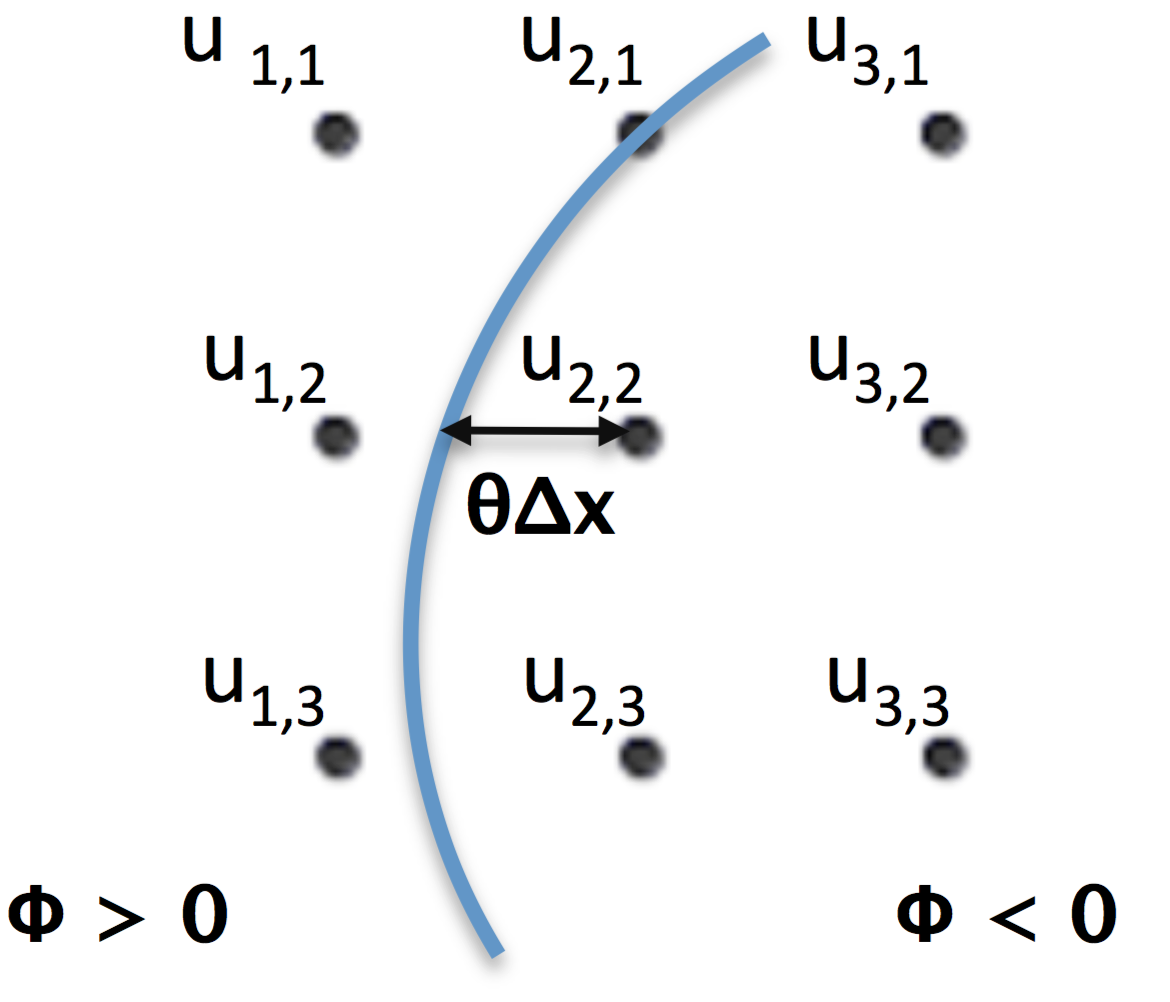
\includegraphics[width=.42 \textwidth]{/Users/meganchang/Desktop/Thesis/images/Ghost_Node_2}
    \caption[Ghost Node Implementation]{Assume the blue arc represents the interface, so that left of the arc $\phi^{n+1} > 0$, and right of the arc $\phi^{n+1} < 0$. Ghost nodes are used to handle any points neighboring the interface. The distance between neighboring points is $\Delta x$, whereas the distance between $u_{2,2}^{n+1}$ and the interface is $\theta \Delta x$.}
    \label{fig:ghost_node}
\end{figure}
Our diffusion equation \eqref{eqn:Crank_discretized} for $u_{2,2}^{n+1}$ is shown below, with the problem points bolded:
\begin{equation}
\begin{aligned}
&\frac{u_{2,2}^{n+1}}{\Delta t} - \frac{1}{2}D \bigg(\frac{\boldsymbol{u_{1,2}^{n+1}}- 2u_{2,2}^{n+1} + u_{3,2}^{n+1}}{\Delta x^2} + \frac{\boldsymbol{u_{2,1}^{n+1}} - 2u_{2,2}^{n+1} + u_{2,3}^{n+1}}{\Delta y^2}\bigg)\\
&= \frac{u_{2,2}^{n}}{\Delta t} + \frac{1}{2}D\bigg(\frac{ \boldsymbol{u_{1,2}^{n}} - 2u_{2,2}^{n} + u_{3,2}^{n}}{\Delta x^2} + \frac{\boldsymbol{u_{2,1}^{n}} - 2u_{2,2}^{n} + {u_{2,3}^{n}}}{\Delta y^2}\bigg)
+ \frac{1}{2}(S_{2,2}^{n+1} + S_{2,2}^{n}).
\end{aligned}
\end{equation}
These bolded values must be replaced with ghost values, $u^G$, found using linear and constant extrapolation, respectively. For example, for $u_{1,2}^{n+1}$, we would have the following two options:
\begin{equation}\label{eqn:ghost_nodes}
\begin{aligned}
u^G_{i-1,j} =& \>\> \frac{u_{\gamma} + (\theta - 1) u_{i,j}}{\theta},\\
u^G_{i-1,j} =& \>\> u_{\gamma},\\
\end{aligned}
\end{equation}
where $u_\gamma$ is the concentration at the interface given by Dirichlet boundary conditions, and $\theta \in [0,1]$ is the fractional distance between $u_{i,j}^{n+1}$ and the interface, as calculated previously in \eqref{eqn:theta^L} and \eqref{eqn:thetas}.

Wherever possible, we will use linear extrapolation (\ref{eqn:ghost_nodes}a) to calculate our ghost value. However, one will notice that (\ref{eqn:ghost_nodes}a) behaves poorly for small $\theta$. Thus, when $\theta < \Delta x$, we need to use constant extrapolation (\ref{eqn:ghost_nodes}b) to ensure stability. To do so, we would reassign the interface to this point, so that $\phi = 0$. So, if the interface did not fall exactly on the grid point $u^{n+1}_{2,1}$ in Figure \ref{fig:ghost_node}, $\theta$ would be considered small enough to use (\ref{eqn:ghost_nodes}b). This second-order-accurate perturbation of the interface location (also known as artificial boundary perturbation) does not degrade the overall second-order accuracy of the solution. Note, that reassigning a point to an interface location makes it a \textit{known value}. Thus, we have to filter through every point to determine if $\theta$ is small enough to be considered on the interface and make this reassignment \textbf{before} we initiate preallocate the size of $\vec{A}$.

Finally, for the case shown in Figure \ref{fig:ghost_node}, we end up with the following linear equation where the ghost values have been included:
\begin{equation}\label{eqn:Crank_dat_ghost}
\begin{aligned}
\frac{u_{2,2}^{n+1}}{\Delta t} - \frac{1}{2}D\bigg(\frac{   \boldsymbol{\frac{(1-\theta)}{\theta} u_{2,2}^{n+1}}
 - 2u_{2,2}^{n+1} + u_{3,2}^{n+1}}{\Delta x^2} + \frac{-2u_{2,2}^{n+1} + u_{2,3}^{n+1}}{\Delta y^2}\bigg)\\
= \frac{u_{2,2}^{n}}{\Delta t} + \frac{1}{2}D\bigg(\frac{   \boldsymbol{\frac{(1-\theta)}{\theta} u_{2,2}^{n}}    - 2u_{2,2}^{n} + u_{3,2}^{n}}{\Delta x^2} + \frac{ - 2u_{2,2}^{n} + {u_{2,3}^{n}}}{\Delta y^2}\bigg)\\
+ \frac{1}{2}(S_{2,2}^{n+1} + S_{2,2}^{n}) + \frac{1}{2} D\bigg(\frac{\boldsymbol{\frac{u_{\gamma}^{n+1}+u_{\gamma}^{n}}{\theta}}}{\Delta x^2} + \frac{\boldsymbol{u_{\gamma}^{n+1}+u_{\gamma}^{n}}}{\Delta y^2}\bigg).
\end{aligned}
\end{equation}
For the ghost value replacing $u_{1,2}^{n+1}$, we must alter two $\vec{A}$ values \eqref{eqn:Crank_coeffs} on the LHS:
\begin{equation}
\begin{aligned}
\text{Left} &= 0,\\
\text{Center} &= 1 + \frac{1}{2}D\bigg(\frac{2 \Delta t}{\Delta x^2} + \frac{2 \Delta t}{\Delta y^2} + \frac{\frac{\theta-1}{\theta}\Delta t}{\Delta x^2}\bigg),
\end{aligned}
\end{equation}
and add $\frac{1}{2} D\bigg( \frac{u_{\gamma}^{n+1}}{\theta \Delta x^2} \bigg)$ to the RHS. We follow the same procedure when we replace $u_{1,2}^n$ with its corresponding ghost value.

Since we use constant extrapolation to replace $u_{2,1}^{n+1}$, only one $\vec{A}$ value \eqref{eqn:Crank_coeffs} changes:
\begin{equation}
\text{Above} = 0,
\end{equation}
and we add $\frac{1}{2}D \bigg(\frac{u_{\gamma}^{n+1}}{\Delta y^2} \bigg)$ to the RHS. We use the same method to replace $u_{2,1}^{n}$ with its corresponding ghost value. 

When linearly extrapolated ghost values are applied to create a sharp interface, we achieve \textbf{symmetric discretization}. This refers to the consistent representation of diffusion between the same two grid nodes. For instance, consider the diffusion between neighboring points $u_{2,2}^{n+1}$ and $u_{3,2}^{n+1}$ in Figure \ref{fig:ghost_node}. The diffusion between the two points are described by the \textbf{Right} coefficient \eqref{eqn:Crank_coeffs} in the discretization at $u_{2,2}^{n+1}$ and the \textbf{Left} coefficient \eqref{eqn:Crank_coeffs} in the discretization at $u_{3,2}^{n+1}$. In the way we have implemented our ghost values, both coefficients would equal $-\frac{1}{2}D\frac{\Delta t}{\Delta x^2}$, hence the symmetric discretization.

Non-symmetric discretization, on the other hand, occurs when one uses quadratic extrapolation to determine ghost values:
\begin{equation}
u^G_{i-1,j} = \>\> \frac{2 u_{\gamma}^{n+1} + (2 \theta^2 - 2) u_{i,j} + (-\theta^2 + 1)u_{i+1,j}}{\theta^2 + \theta}.\\
\end{equation}
In this case, the discretization at $u_{3,2}^{n+1}$ has not changed (i.e. Left = $-\frac{1}{2}D\frac{\Delta t}{\Delta x^2}$), but the discretization at $u_{2,2}^{n+1}$ now includes some factor $\theta$ in the Right coefficient \bigg(i.e. Right = $-\frac{1}{2}D\frac{\Delta t}{\Delta x^2} \bigg(1 + \frac{-\theta^2 + 1}{\theta^2 + \theta} \bigg)\bigg)$. This unequal representation of diffusion between the same two points leads to a non-symmetric discretization, which is computationally more expensive to solve. For this reason, we use linearly extrapolated ghost values.

\section{Accuracy of the Diffusion Solver}

Figure \ref{fig:circles} illustrates our diffusion program working with several different level-sets described by the equations in Table \ref{table:level_set_shapes} on a domain $\Omega = [-1,1]^2$, with a source term  
\begin{equation*}
S(x,y,t) = \cos(x)\sin(x)e^{y}\cos(t) -D(-2\sin(2x)e^{y}\sin(t) + \cos(x)\sin(x)e^{y}\sin(t)),
\end{equation*}
where we use a diffusion coefficient $D = 2$, and ran the simulation to a final time $t = 0.1$. The reason for this somewhat convoluted source term is because we are trying to impose a desired outcome $u_{\text{numerical}}$. To do this, we plug a test function
\begin{equation}
u_{\text{exact}}(x,y,t) = \cos(x)\sin(x)e^{y}\sin(t)
\end{equation}
into the diffusion equation \eqref{eqn:Crank_discretized} and solve analytically for $S$. We can then use $u_{\text{exact}}$ to define initial conditions and Dirichlet boundary conditions, and use the source term to compute a numerical solution, $u_{\text{numerical}}$, that we can compare to $u_\text{exact}$ for error analysis.

Tables \ref{table:Circle_Crank} - \ref{table:Flower_Crank} demonstrate that our diffusion solver has second-order accuracy for all four level-set shapes, where we set $\Delta t = \Delta x$ to ensure that the stringent time step restriction has been alleviated through our implicit method.

\begin{table} [ht]
\caption{Level-Set Functions}\label{table:level_set_shapes}
\centering
\begin{tabular}{c| c}
\hline
Circle      & $\phi(x,y) = \sqrt{x^2 - y^2} - 0.5$\\ \hline
Diamond     & $\phi(x,y) = |x| + |y| - 0.5$\\ \hline
Fat Flower  & $\phi(x,y) = (x-0.02\sqrt{5})^2 + (y-0.02\sqrt{5})^2 - (0.5 + 0.2\>\sin(5\>\theta(x,y)))^2$\\ \hline
Thin Flower & $\phi(x,y) = \sqrt{x^2 + y^2} - (0.35 + 0.28\>\cos(9\>\theta(x,y)))$ \\\hline
\end{tabular}
\end{table}

\begin{figure}[!h]
\centering
\subfigure[Circle]{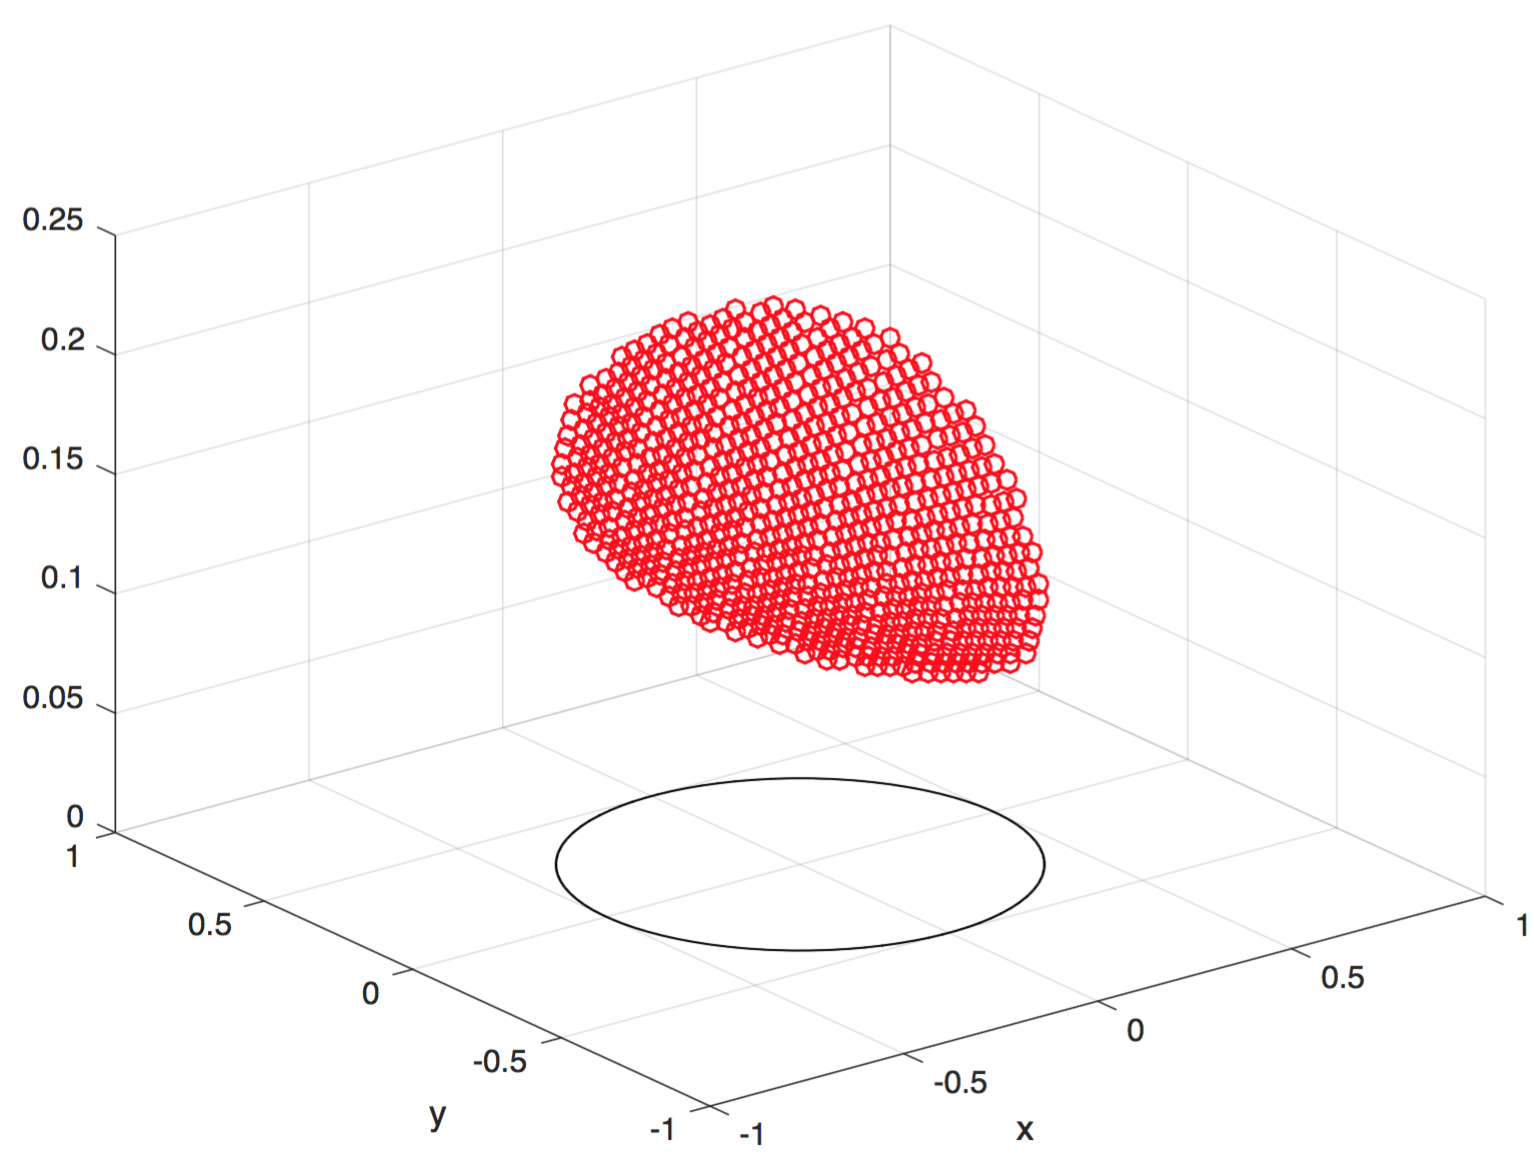
\includegraphics[width=.48\textwidth]{/Users/meganchang/Desktop/Thesis/images/Diffusion_Plot3_Circle.png}} \quad
\subfigure[Diamond]{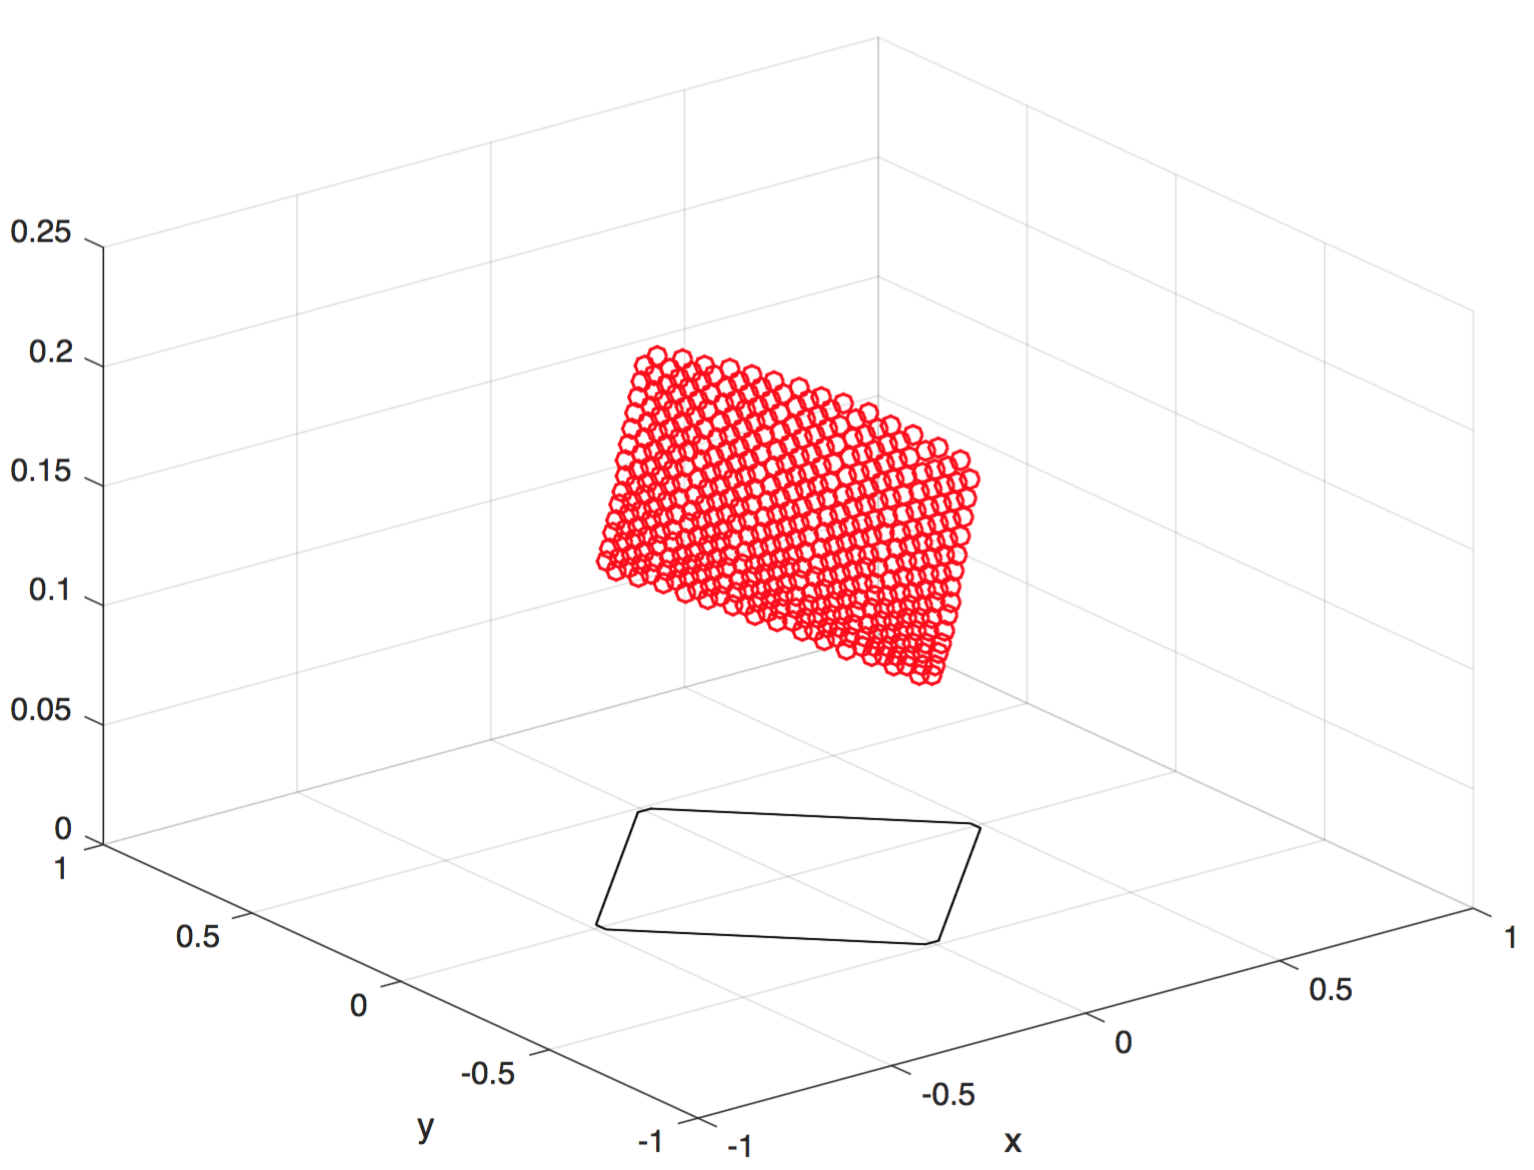
\includegraphics[width=.48\textwidth]{/Users/meganchang/Desktop/Thesis/images/Diffusion_Plot3_Diamond.png}}\\
\subfigure[Fat-Petal Flower]{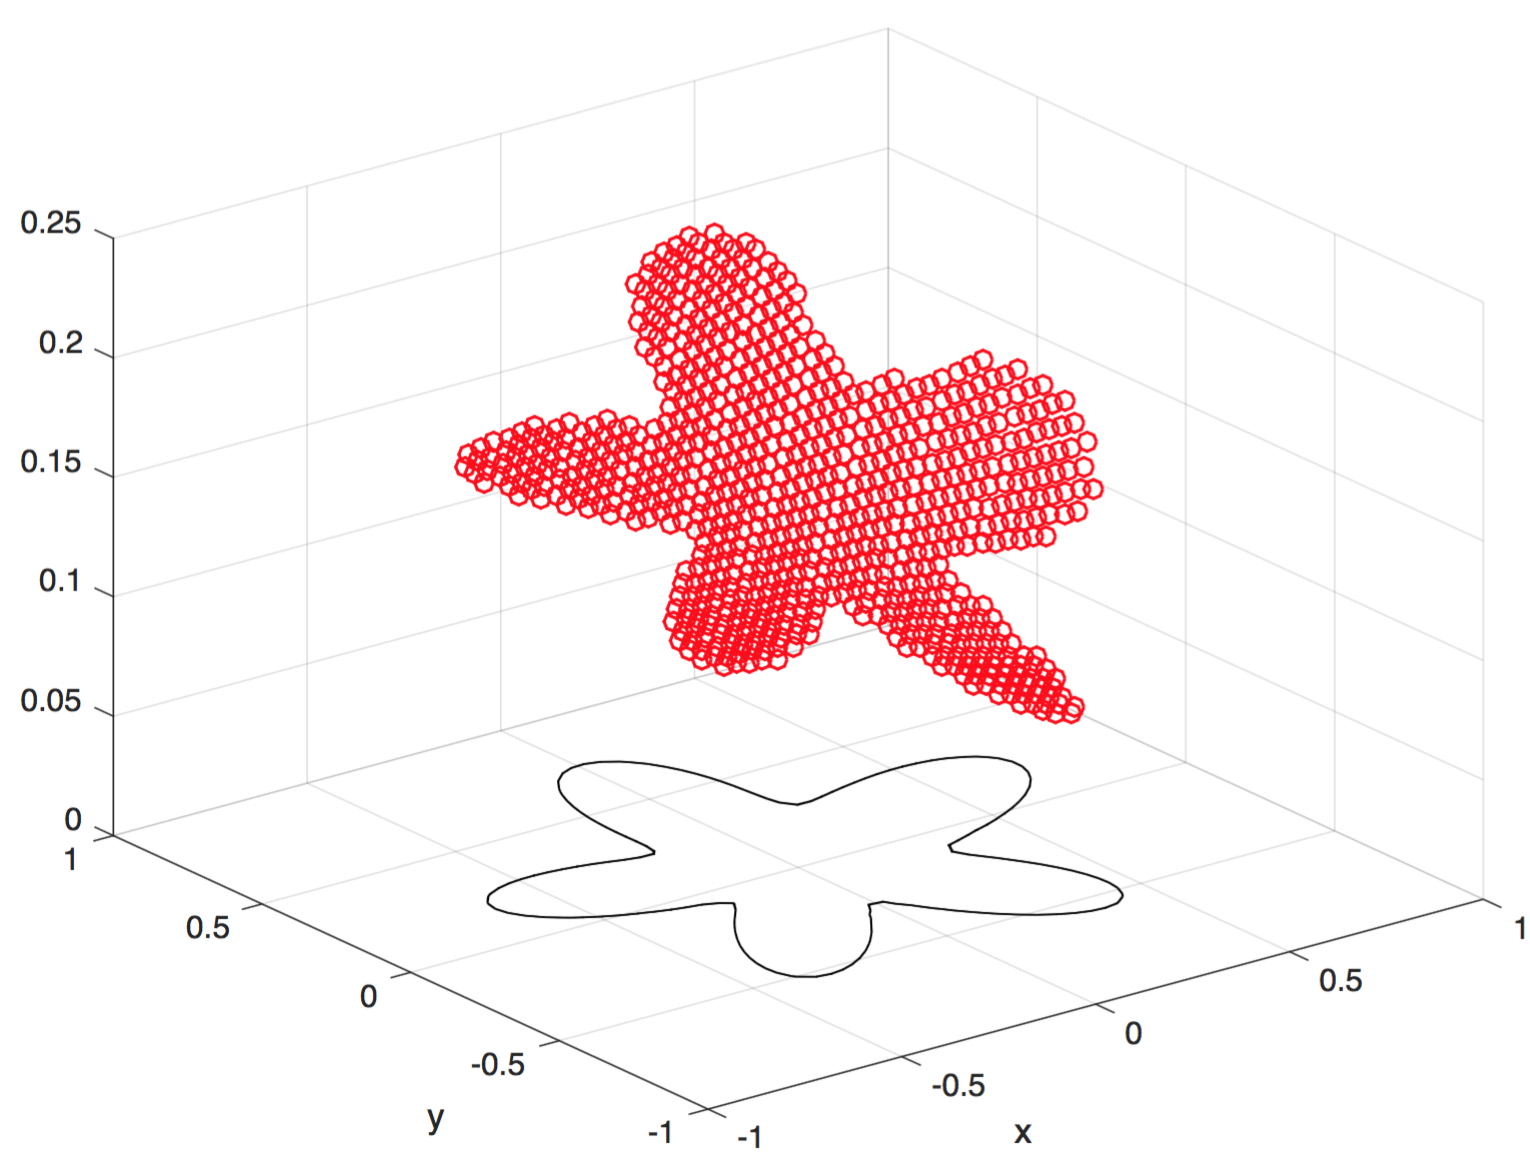
\includegraphics[width=.48\textwidth]{/Users/meganchang/Desktop/Thesis/images/Diffusion_Plot3_Flower.png}} \quad
\subfigure[Thin-Petal Flower]{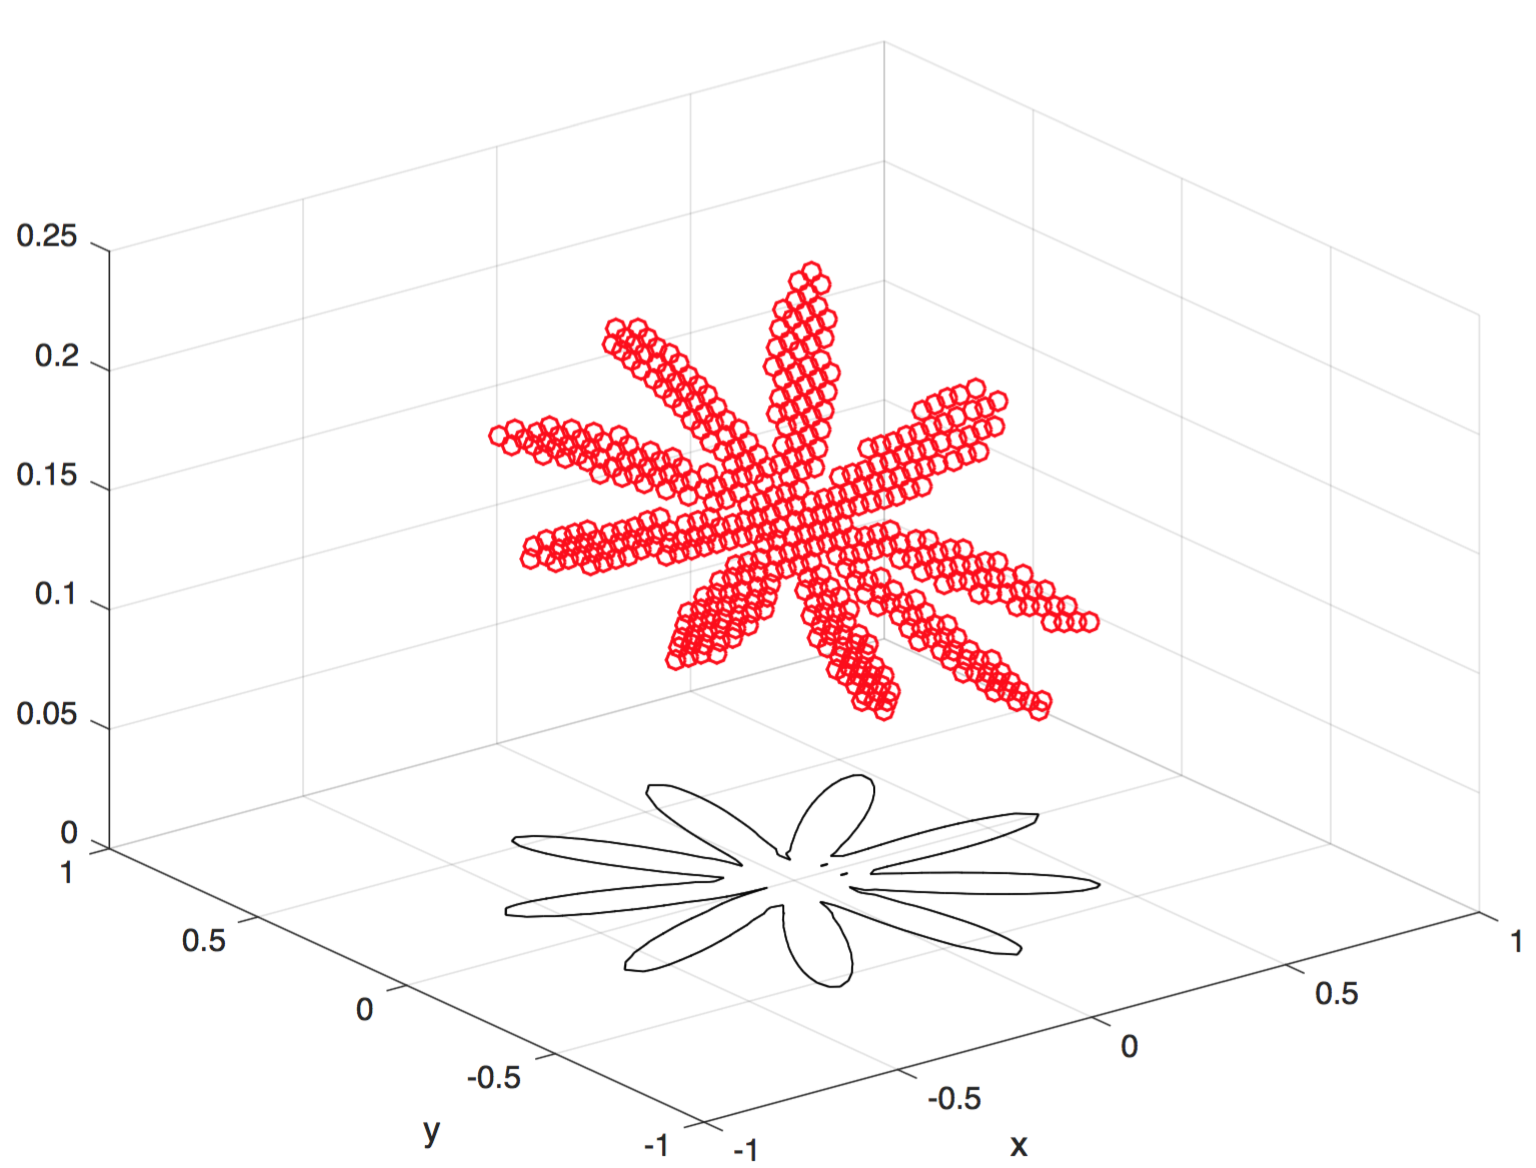
\includegraphics[width=.48\textwidth]{/Users/meganchang/Desktop/Thesis/images/Diffusion_Plot3_Crazy.png}}
  \caption[2D Heat Equation with Dirichlet Boundary Conditions for Various Level-Sets]{Two-dimensional solutions of the heat equation with Dirichlet boundary conditions solved in only the $\Omega^-$ subdomain. We use the same source term for each level-set shape (described by the equations in Table \ref{table:level_set_shapes}) on a 60$\times$60 grid resolution to impose our desired outcome $u_{\text{numerical}}$ for error analysis.}
  \label{fig:circles}
\end{figure}

\clearpage
\begin{table} [!h]
\caption{Circle 2D Heat Equation - Crank-Nicholson - $\Delta t = \Delta x$}\label{table:Circle_Crank}
\centering
\begin{tabular}{c c c c c}
\hline
Grid Resolution & $L^1$ - error           & Order  & $L^{\infty}$ - error        & Order \\ \hline
81$\times$81      & $1.616 \times 10^{-6}$  &   -    & $1.068 \times 10^{-5}$   &  -    \\
161$\times$161   & $4.327 \times 10^{-7}$  &  1.90  & $2.869 \times 10^{-6}$   & 1.90  \\
321$\times$321   & $1.091 \times 10^{-7}$  &  1.99  & $7.671 \times 10^{-7}$   & 1.90 
\end{tabular}
\end{table}

\begin{table} [!h]
\caption{Diamond 2D Heat Equation - Crank-Nicholson - $\Delta t = \Delta x$}
\centering
\begin{tabular}{c c c c c}
\hline
Grid Resolution & $L^1$ - error           & Order  & $L^{\infty}$ - error        & Order \\ \hline
81$\times$81     & $3.408 \times 10^{-8} $ &   -    & $1.716 \times 10^{-7}$   &  -    \\
161$\times$161   & $8.319 \times 10^{-9} $ &  2.03  & $4.225 \times 10^{-8}$   & 2.02  \\
321$\times$321   & $2.075 \times 10^{-9} $ &  2.00  & $1.060 \times 10^{-8}$  & 2.00  
\end{tabular}
\end{table}

\begin{table} [!h]
\caption{Fat-Petal Flower 2D Heat Equation - Crank-Nicholson - $\Delta t = \Delta x$}
\centering
\begin{tabular}{c c c c c}
\hline
Grid Resolution & $L^1$ - error           & Order  & $L^{\infty}$ - error        & Order \\ \hline
81$\times$81     & $2.291 \times 10^{-6}$  &   -    & $2.517 \times 10^{-5}$   &  -  \\
161$\times$161   & $4.704 \times 10^{-7}$  &  2.28  & $6.856 \times 10^{-6}$   & 1.88\\
321$\times$321   & $1.037 \times 10^{-7}$ &  2.18  & $2.099 \times 10^{-6}$   & 1.71\\
\end{tabular}
\end{table}

\begin{table} [!h]
\caption{Thin-Petal Flower 2D Heat Equation - Crank-Nicholson - $\Delta t = \Delta x$}\label{table:Flower_Crank}
\centering
\begin{tabular}{c c c c c}
\hline
Grid Resolution & $L^1$ - error           & Order  & $L^{\infty}$ - error        & Order \\ \hline
81$\times$81     & $2.061 \times 10^{-5}$  &   -    & $2.933 \times 10^{-4}$   &  -    \\
161$\times$161   & $5.284 \times 10^{-6}$  &  1.96  & $7.207 \times 10^{-5}$   & 2.02  \\
321$\times$321   & $1.296 \times 10^{-6}$ &  2.03  & $1.303 \times 10^{-5}$   & 2.47  \\
\end{tabular}
\end{table}

%=== Chapter 4 ============================================
\chapter{Calculating the Interface Velocity} \label{section:Interface_Velocity}

The Stefan problem is a free boundary problem for which we solve for both a changing concentration $u$ and changing domain shape $\Omega^-$. Here, we discuss how we account for the changing $\Omega^-$ by using the level-set advection equation's  \eqref{eqn:level_set}  interface velocity
\begin{equation}\label{eqn:int_velocity}
\vec{v} = [D \nabla u]_{\gamma}
\end{equation}
to find our new $\phi^{n+1}$, where $D$ is the diffusion coefficient, $\nabla u$ is the gradient of concentration, and $[\cdot]_\gamma$ denotes a jump across the interface. In a more explicit representation, we are looking for
\begin{equation}
\begin{aligned}
v_x &= D_\text{in} \bigg(\frac{\partial u_\text{in}}{\partial x}\bigg) - D_\text{out} \bigg(\frac{\partial u_\text{out}}{\partial x}\bigg),\\
v_y &= D_\text{in} \bigg(\frac{\partial u_\text{in}}{\partial y}\bigg) - D_\text{out} \bigg(\frac{\partial u_\text{out}}{\partial y}\bigg),
\end{aligned}
\end{equation}
where $v_{x}$ and $v_{y}$ represent the $x$ and $y$ components of the interface velocity, respectively. Further, $D_\text{in}$ and $u_\text{in}$ refer to values in the subdomain $\Omega^-$, whereas $D_\text{out}$ and $u_\text{out}$ refer to values in the subdomain $\Omega^+$.

To compute the gradient of $\phi$, we use centered finite differencing in space
\begin{equation} \label{eqn:central_diff}
\nabla \phi  = \bigg( \phi_x, \phi_y \bigg) =\>\>  \bigg( \> \frac{\phi_{i+1,j} - \phi_{i-1,j}}{2\Delta x}, \frac{\phi_{i,j+1} - \phi_{i,j-1}}{2\Delta y} \> \bigg).
\end{equation}

We use central differencing again to find the gradient of $u$
\begin{equation} \label{eqn:nablau}
\nabla u  = \bigg( u_x, u_y \bigg) =\>\>  \bigg( \> \frac{u_{i+1,j} - u_{i-1,j}}{2\Delta x}, \frac{u_{i,j+1} - u_{i,j-1}}{2\Delta y} \> \bigg).
\end{equation} 

It is in this step that our Stefan solver becomes first-order accurate. This becomes evident when one considers the gradient of $u$ with the orders included. Remember that our solution for $u$ is limited by the second-order accurate diffusion solver so that each $u$ has an associated error $O(\Delta x^2)$. Central differencing is second-order accurate as well, so if we consider these orders of error, our equation appears as:
\begin{equation}
\frac{\partial u}{\partial x} = \frac{u_{i+1,j} + O(\Delta x^2)-u_{i-1,j}+ O(\Delta x^2)}{2 \Delta x} + O(\Delta x^2),
\end{equation}
which reduces to a first-order accurate derivative since 
\begin{equation}
\frac{\partial u}{\partial x} = \frac{u_{i+1,j} -u_{i-1,j}}{2 \Delta x} + O(\Delta x) + O(\Delta x^2),
\end{equation}
simply becomes
\begin{equation}
\frac{\partial u}{\partial x} = \frac{u_{i+1,j} -u_{i-1,j}}{2 \Delta x} + O(\Delta x).
\end{equation}
This occurs because the smaller magnitude of error $O(\Delta x^2)$ will be dominated by the first-order error $O(\Delta x)$. As one can see, central differencing will lower the order of accuracy by one since $\Delta x$ is in the denominator. This means at best, with a second-order accurate solution, one can achieve first-order accuracy. And since our interface velocity is first-order, our Stefan solver is first-order accurate.

Seeing that we need to find gradients at the interface in both the reacted $\Omega^-$ and unreacted $\Omega^+$ domains, we implement a third-order extrapolation method to extrapolate values of $u$ in the layer of grid nodes near the interface. As we discussed before, our Dirichlet boundary conditions allow us to decouple the solutions across each region. That is to say, we can store the two different region concentrations $u_{\text{in}}$ and $u_{\text{out}}$, separately. For $u_{\text{in}}$, we extrapolate from the  $\Omega^-$ domain a small layer into the $\Omega^+$ domain; and for $u_{\text{out}}$, we extrapolate from the $\Omega^+$ domain a small layer into the $\Omega^-$ domain. Thus, we will create a small band, or layer of points, around the interface for which we have valid extrapolated values for both $u_{\text{in}}$ and $u_{\text{out}}$.

Now, we can calculate the gradients at the interface and calculate the interface velocity. Although this velocity is only needed at the interface, in practice it is easier to simply compute the interface velocity in the entire domain. 

\section{Third-Order Extrapolation Method}

We implement the third-order extrapolation method presented by Aslam in [5]. This higher-order extrapolation method is necessary for two reasons. First, we require accurate gradient values $\nabla u$ at the interface to calculate the interface velocity $\vec{v}$. Second, as the phase boundary moves to include new grid nodes, we need to have valid values of $u_{\text{in}}$ at these new grid nodes in order to employ the Crank-Nicholson method for our diffusion solver. Therefore, we need to extrapolate $u$ quadratically in a band about the interface. To achieve this, we first calculate the second normal directional derivative of $u$ in our domain $\Omega^-$
\begin{equation}  
\begin{aligned}
u_{nn} = \vec{n} \cdot \nabla(\vec{n} \cdot \nabla u),
\end{aligned}
\end{equation}
where $\nabla u$ is defined by \eqref{eqn:nablau} and $\vec{n}$ is the local unit normal to the interface $(\vec{n} = \frac{\nabla \phi}{|\nabla \phi|})$, or in more explicit representation
\begin{equation}\label{eqn:normal}
\vec{n}\>\> = \bigg( n_1,n_2 \bigg) = \>\>\bigg( \> \frac{\phi_x}{\sqrt{\phi_x^2 + \phi_y^2}}\>\>,\>\> \frac{\phi_y}{\sqrt{\phi_x^2 + \phi_y^2}} \> \bigg).
\end{equation}
Then, we solve the following partial differential equations for $u_{nn}$, $u_n$, and $u$, respectively, using an iterative solver
\begin{equation}  
\begin{aligned}
\frac{\partial u_{nn}}{\partial \tau} \> + \> &H(\phi,u_{nn})(\vec{n} \cdot \nabla u_{nn}\>\>\>\>\>\>\>\>\>\>\>\>\>) = 0,\\
\frac{\partial u_{n}\>\>}{\partial \tau} \> + \>&H(\phi,u_{n }\>\>)(\vec{n} \cdot \nabla u_{n}\>\>-u_{nn}) = 0,\\
\frac{\partial u\>\>\>\>}{\partial \tau} \> + \> &H(\phi,u\>\>\>\>)(\vec{n} \cdot \nabla u\>\>\>\> - u_n\>\>) = 0,\\
\end{aligned}
\end{equation}
where the Heaviside functions $H$ are defined below, and $\tau$ is a fictitious time. Only a few iterations are required to propagate the solution out in the layer of grid points near the interface. Notice, that the three equations follow the same format whereby we impose our desired normal derivative by subtracting it from the parenthesized term ($\vec{n} \cdot \nabla u$). Hence, to impose extrapolation in the normal direction, we begin by subtracting zero from $(\vec{n} \cdot \nabla u_{nn})$. Now, we have our second directional derivative defined and can use it to compute the first directional derivative $u_{n}$ by solving our second PDE. And finally, we compute $u$ in our third PDE with the imposed first directional derivative $u_n$. In semi-discretized form, we have
\begin{equation}  
\begin{aligned}
\frac{d}{d \tau}u_{nn} + H(\phi,u_{nn})(n_x^+D_x^-u_{nn} + n_x^-D_x^+u_{nn} + n_y^+D_y^-u_{nn} + n_y^-D_y^+u_{nn}) &= 0,\\
\frac{d}{d \tau}u_{n}\>\> + H(\phi,u_{n)\>\>}(n_x^+D_x^-u_{n}\>\> + n_x^-D_x^+u_{n}\>\> + n_y^+D_y^-u_{n}\>\> + n_y^-D_y^+u_{n}\>\>) &= H(\phi,u_n)u_{nn},\\
\frac{d}{d \tau}u\>\>\>\> + H(\phi,u\>\>\>\>)(n_x^+D_x^-u\>\>\>\> + n_x^-D_x^+u\>\>\>\> + n_y^+D_y^-u\>\>\>\> + n_y^-D_y^+u\>\>\>\>) &= H(\phi,u)u_n\>\>,
\end{aligned}
\end{equation}
where $n_x^+$ = max$(n_x,0)$, $n_x^-$ = min$(n_x,0)$, $n_y^+$ = max$(n_y,0)$, and $n_y^-$ = min$(n_y,0)$. Also, we use the first-order one-sided finite differences \eqref{eqn:directional_derivatives} to calculate our directional derivatives.

The Heaviside functions $H(\phi,x)(v_j)$ label each point as having a known or unknown value for $x$ at a point $v_j$, where zero corresponds to a known and one corresponds to an unknown. For example, since we know $u$ at all points in $\Omega^-$, $H(\phi, u)(v_j) = 0$ at all points $v_j$ where $\phi < 0$, while $H(\phi, u)(v_j) = 1$ for all points $v_j$ where $\phi \ge 0$. (Recall that since we reassign values of $\phi$ to zero when $\theta$ is too small, it is better to consider these $u$ values to be unknown, so that we can extrapolate values at these points where $\phi = 0$. We found this produced more robust and accurate results.)

To calculate the derivatives $u_x$ and $u_y$ using central differencing, we need all four neighboring points $v_i$ to be contained in $\Omega^-$. In other words, we need $H(\phi, u)(v_i) = 0$ for all four neighbors $v_i$ of $v_j$ to set $H(\phi, u_n)(v_j) = 0$. Likewise, we need all four neighboring points $v_i$ to have known first derivatives in order to use central differencing to find the second derivatives ($u_{xx}$ and $u_{yy}$). To summarize, the Heaviside functions are defined as
 \begin{equation*}
H(\phi,u_{nn})(v_i) = 
\begin{cases}
    0 & \text{if } H(\phi,u_n)(v_j) = 0 \text{ for all } v_j \in \text{ngbd}(v_i),\\ 
    1 & \text{otherwise},
\end{cases}
\end{equation*}
\begin{equation}
H(\phi,u_n \>\>)(v_i)  = 
\begin{cases}
    0 & \text{if } H(\phi,u)(v_j) = 0 \text{ for all } v_j\in \text{ngbd}(v_i), \>\> \\ 
    1 & \text{otherwise},
\end{cases}
\end{equation}
\vspace{0.1in}
\begin{equation*}
H(\phi,u \>\>\>\>)(v_i) = 
\begin{cases}
    0 & \text{if $\phi(v_i) < 0$}, \>\>\>\>\>\>\>\>\>\>\>\>\>\>\>\>\>\>\>\>\>\>\>\>\>\>\>\>\>\>\>\>\>\>\>\>\>\>\>\>\>\>\>\>\>\>\>\>\>\>\>\>\>\> \\ 
    1 & \text{otherwise},
\end{cases}
\end{equation*}

Figure \ref{fig:extrapolation} demonstrates visually what this third-order extrapolation method achieves. 


\begin{figure} [!h]
\centering
\subfigure[Initial Data]{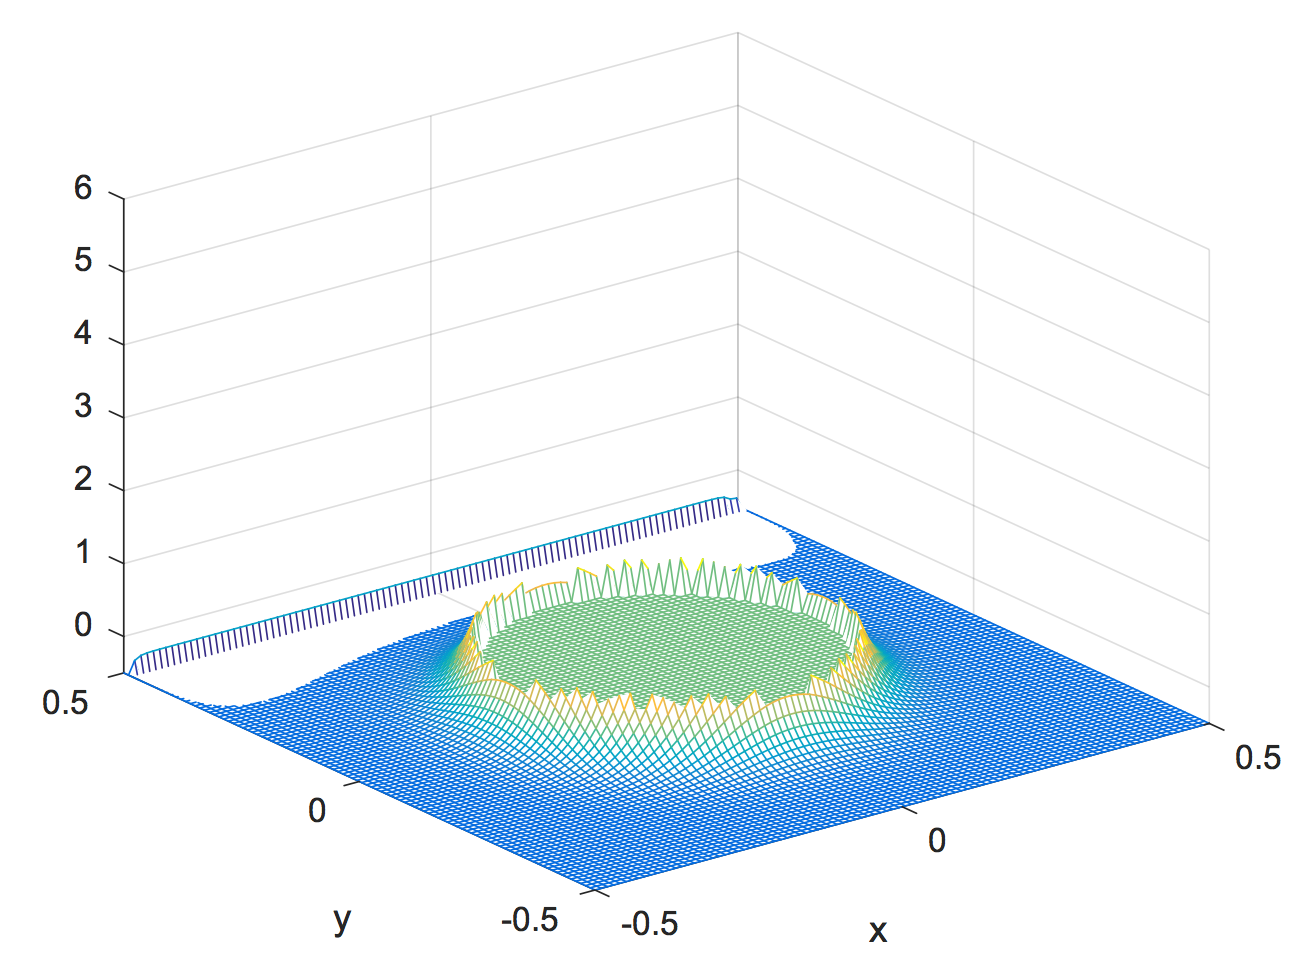
\includegraphics[width=.44\textwidth]{/Users/meganchang/Desktop/Thesis/images/Extrapolate_Before.png}} \\
\subfigure[15 iterations]{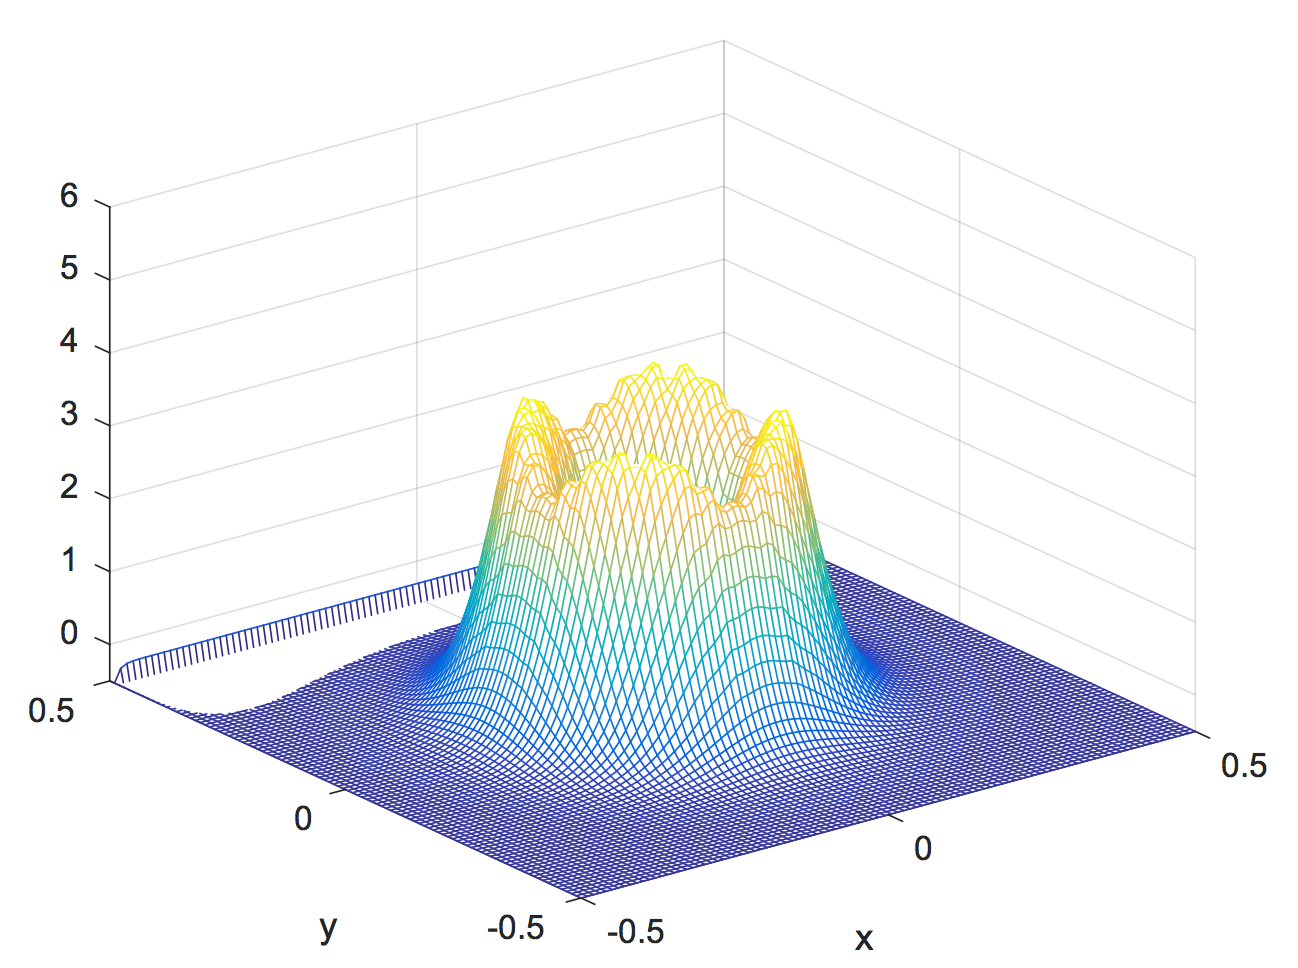
\includegraphics[width=.44\textwidth]{/Users/meganchang/Desktop/Thesis/images/Extrapolate_After.png}}\\
\subfigure[30 iterations]{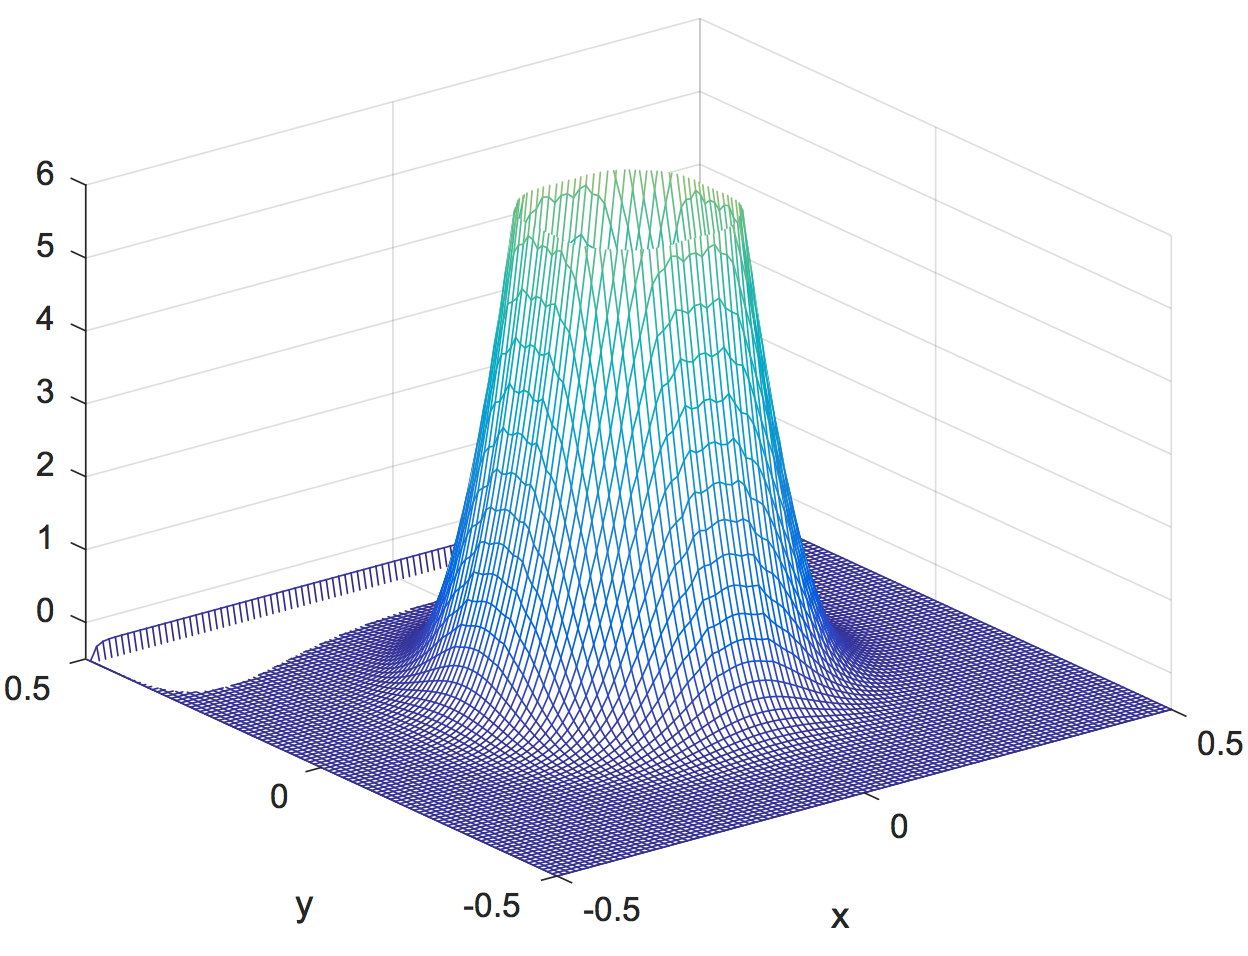
\includegraphics[width=.44\textwidth]{/Users/meganchang/Desktop/Thesis/images/Extrapolate_After30.png}}
  \caption[Third-Order Extrapolation Method]{We begin with $u$ defined everywhere except inside the circle at the center. As we execute more iterations, the extrapolated solution gets propagated further. In addition, it becomes more accurate so that the points shown in (b) are now more accurate in (c).}
  \label{fig:extrapolation}
\end{figure}

\section{Accuracy Analysis}

Since we are only interested in the points near the interface, we compare the exact solution to our extrapolated solution for only points in $\Omega^+$ where $|\phi| < 2 \Delta x$. Furthermore, we investigated the necessary amount of iterations needed for our solution to converge in this band, with the goal of maximizing the order of accuracy, while minimizing the amount of iterations to save computational effort. Figure \ref{fig:Third_Order_Iterations} plots the error analysis in $L^1$ and $L^\infty$ against the number of iterations. We perform this error analysis for the four level-sets described in Table \ref{table:level_set_shapes} to demonstrate the third-order extrapolation method's convergence dependency on both grid resolution and level-set smoothness. Also, note that we had to reinitialize the level-sets before third-order accurate extrapolation could be achieved.

\begin{figure} [!h]
\centering
\subfigure[Circle $L^1$]{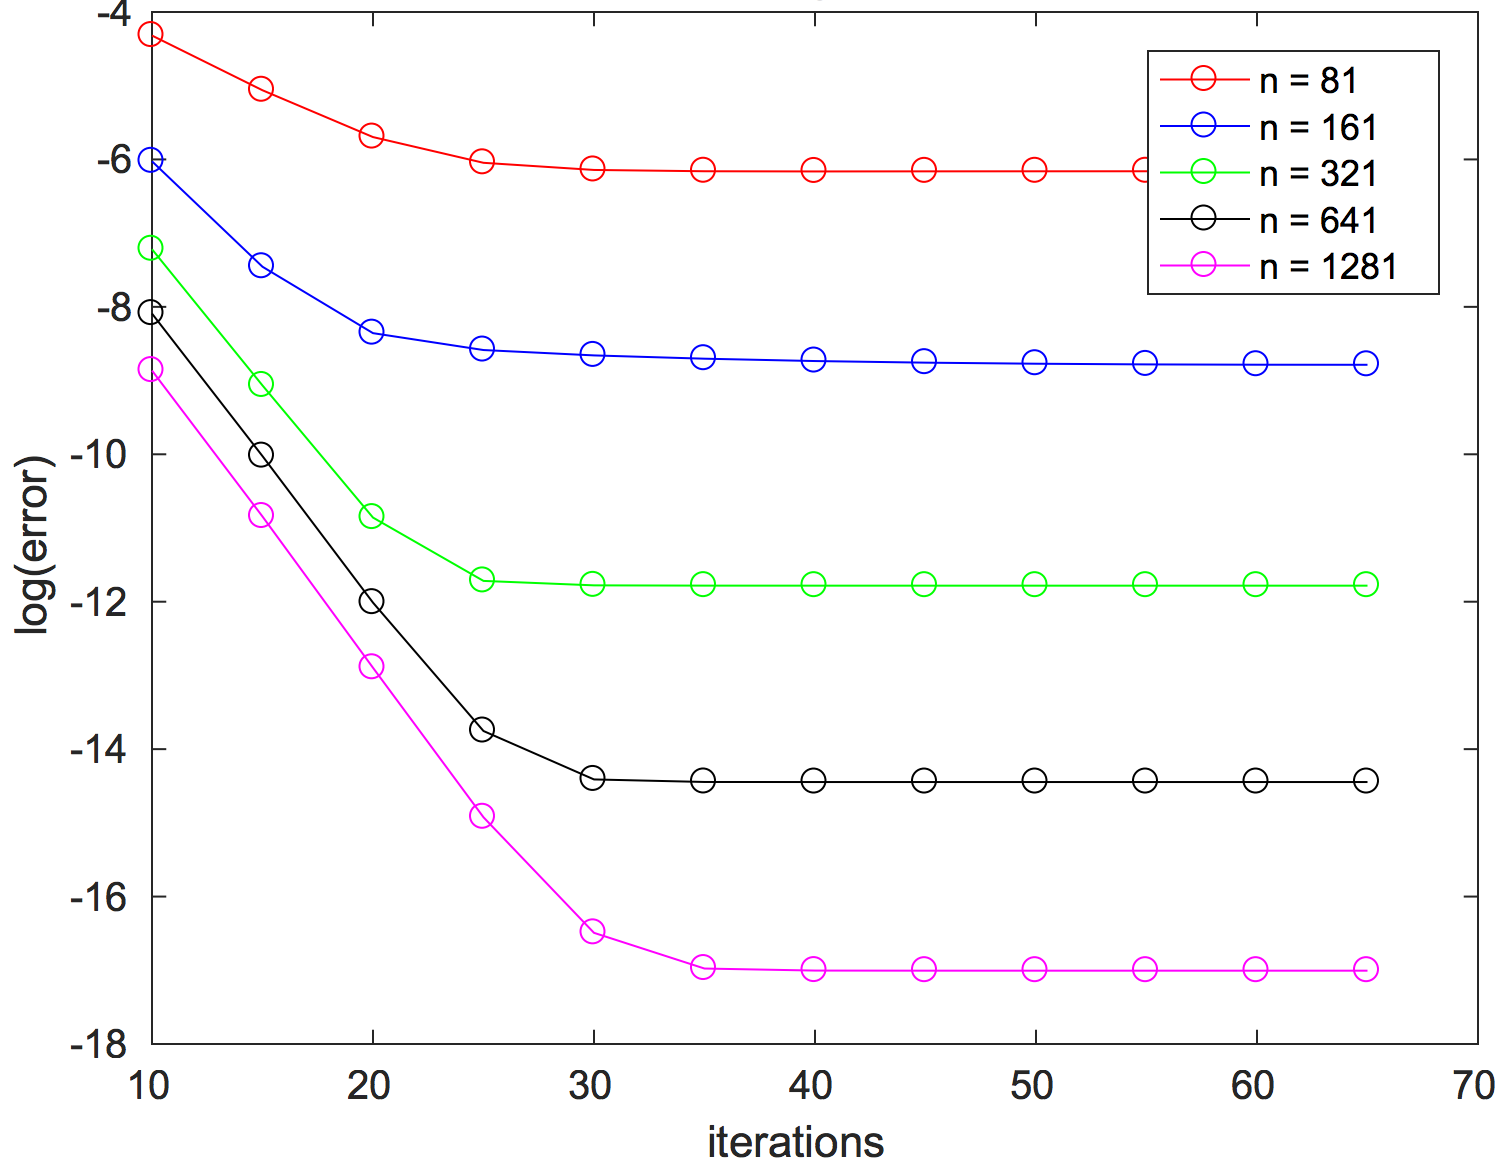
\includegraphics[width=.3\textwidth]{/Users/meganchang/Desktop/Thesis/images/Iterations_Circle_1.png}} \quad
\subfigure[Circle $L^\infty$]{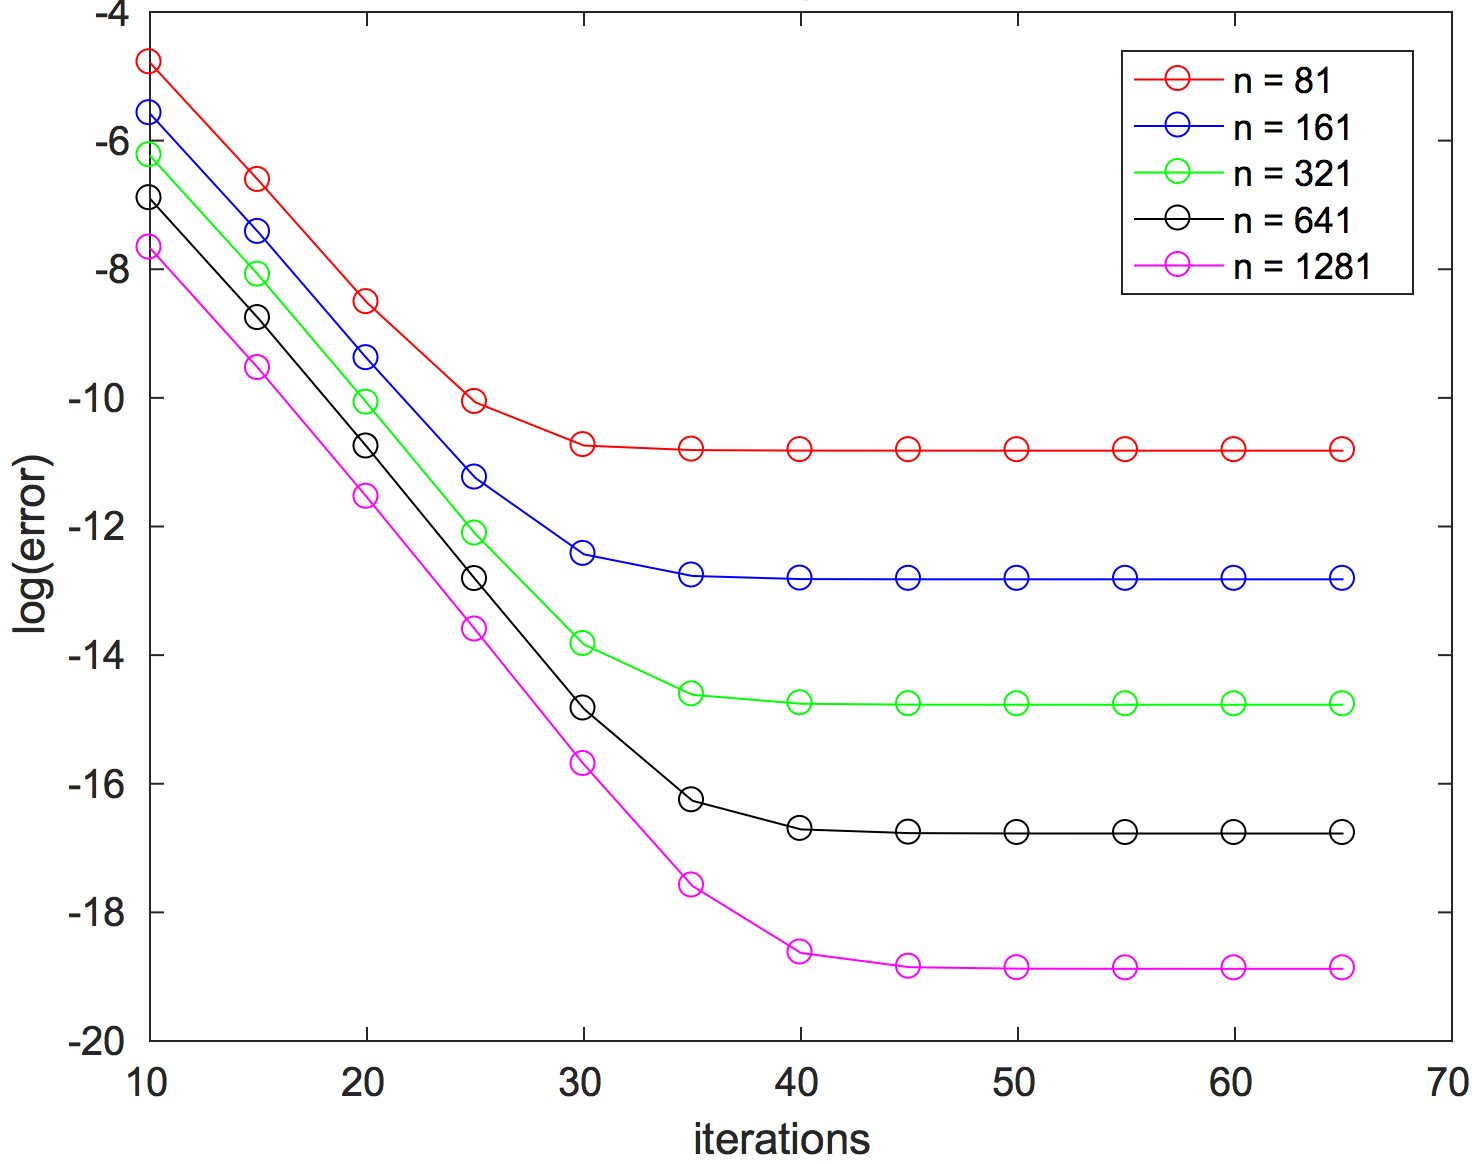
\includegraphics[width=.3\textwidth]{/Users/meganchang/Desktop/Thesis/images/Iterations_Circle_inf.png}}\\
\subfigure[Diamond $L^1$]{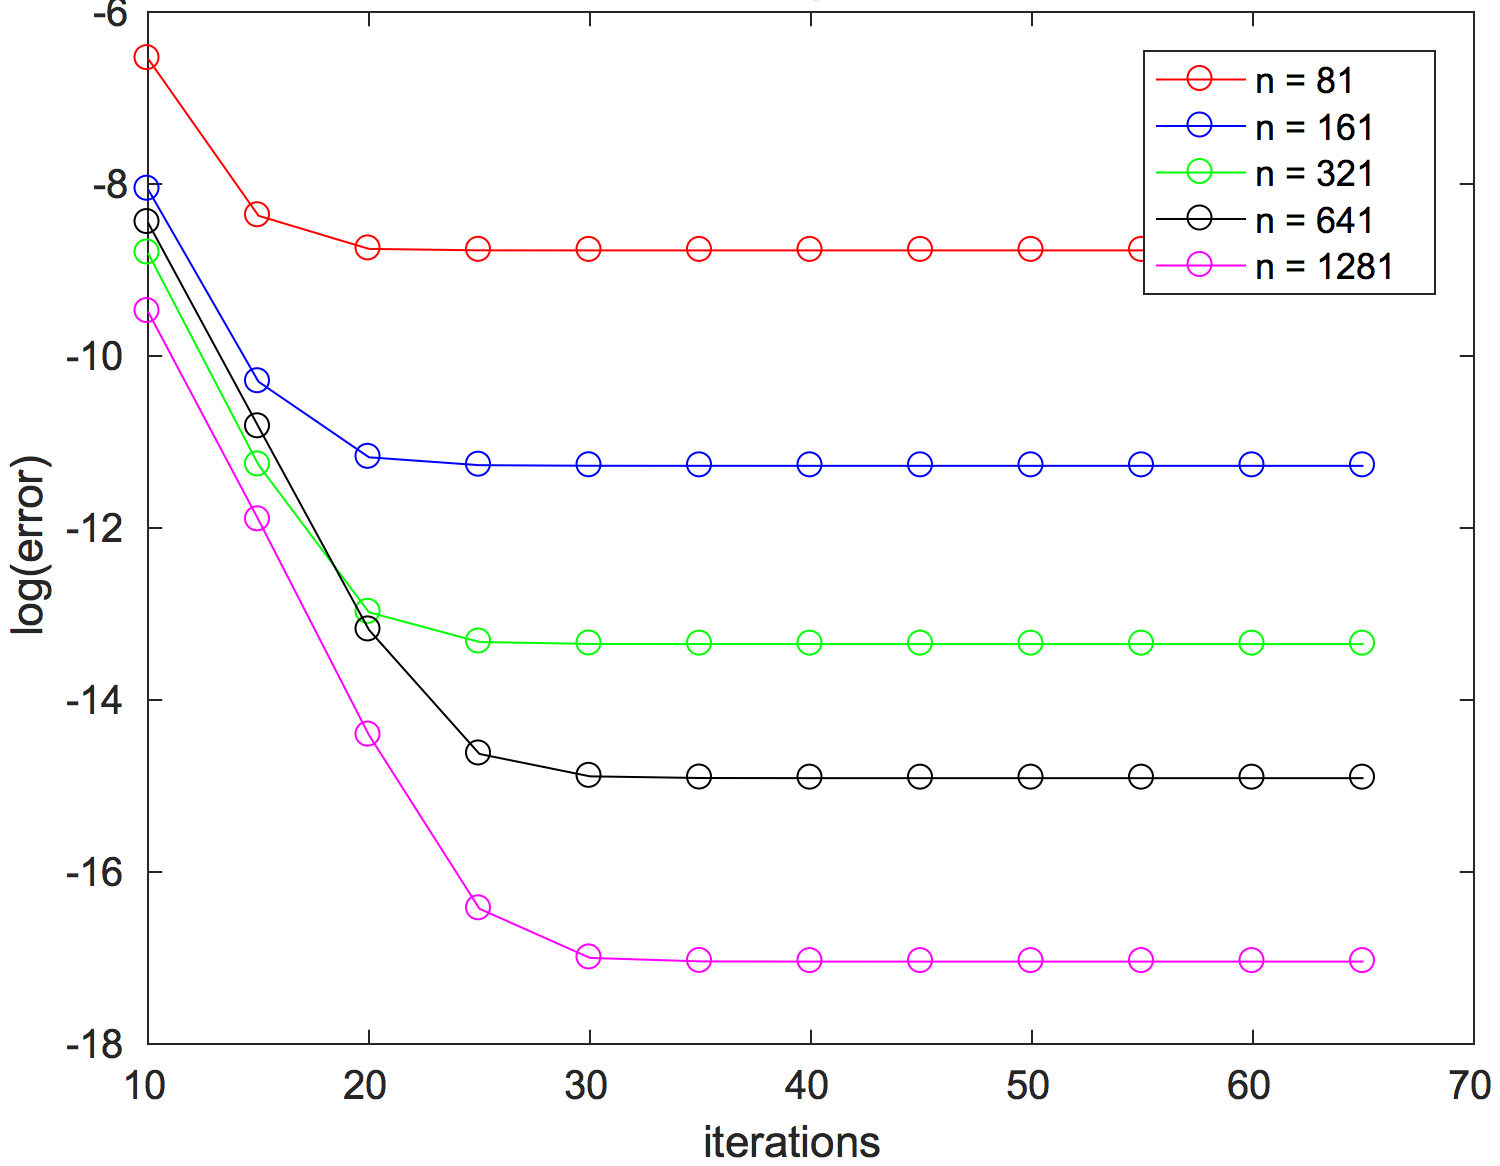
\includegraphics[width=.3\textwidth]{/Users/meganchang/Desktop/Thesis/images/Iterations_Diamond_1.png}} \quad
\subfigure[Diamond $L^\infty$]{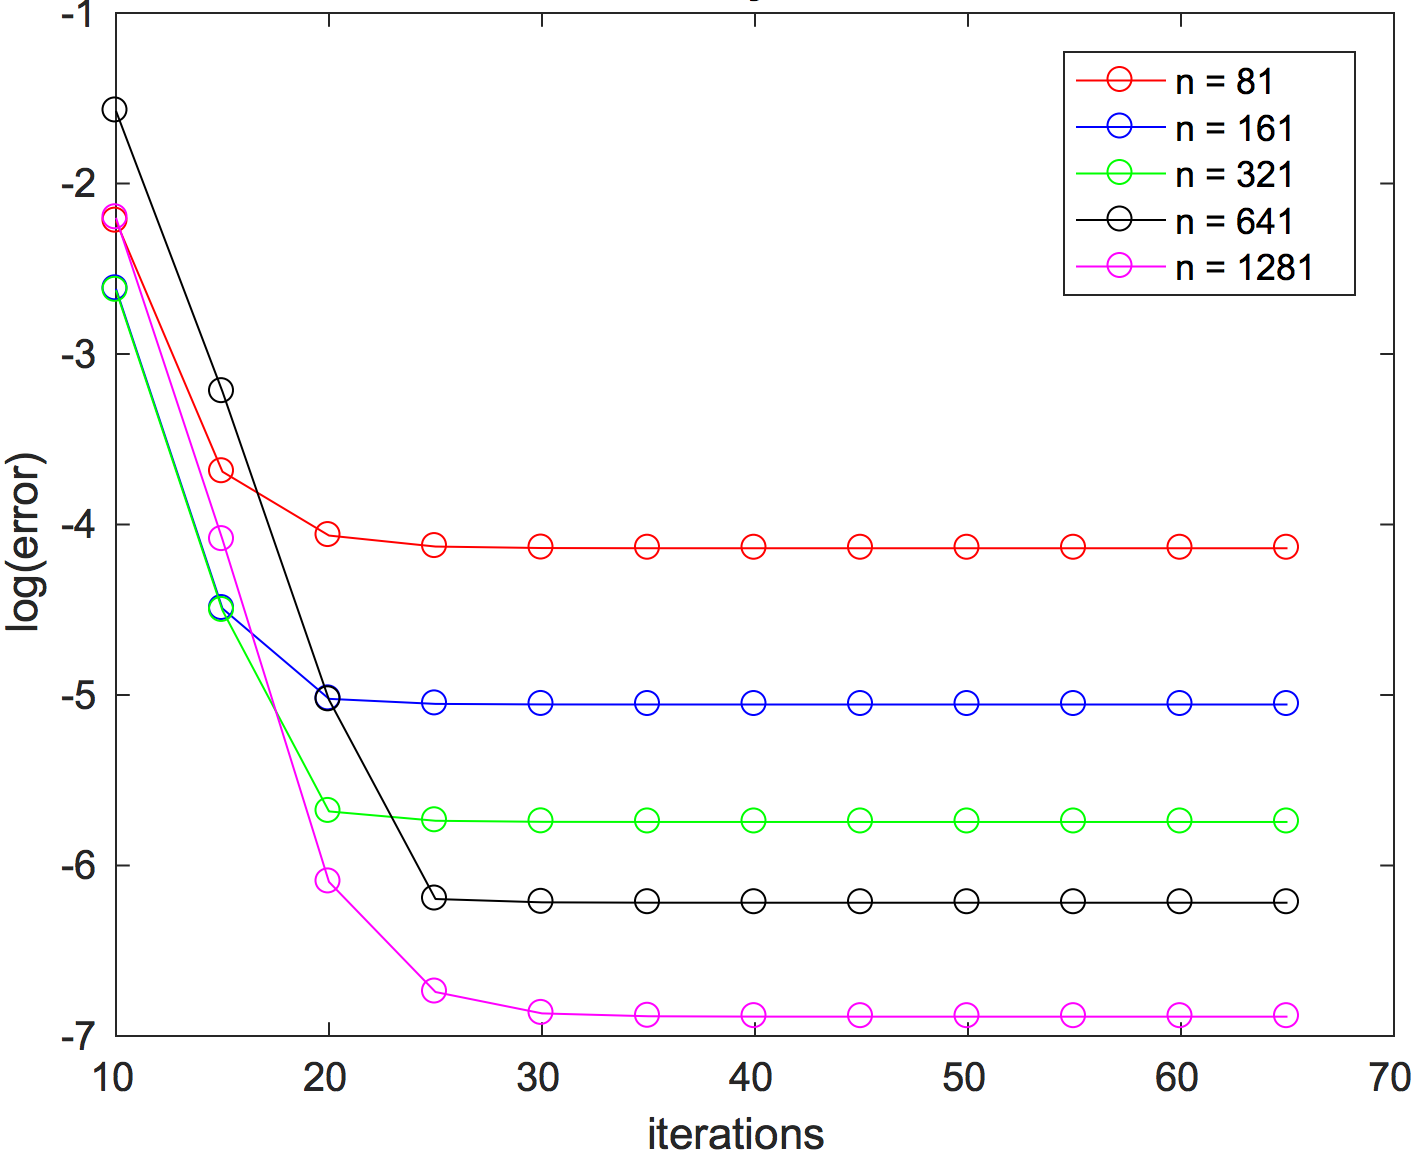
\includegraphics[width=.3\textwidth]{/Users/meganchang/Desktop/Thesis/images/Iterations_Diamond_inf.png}}\\
\subfigure[Fat-Petal Flower $L^1$]{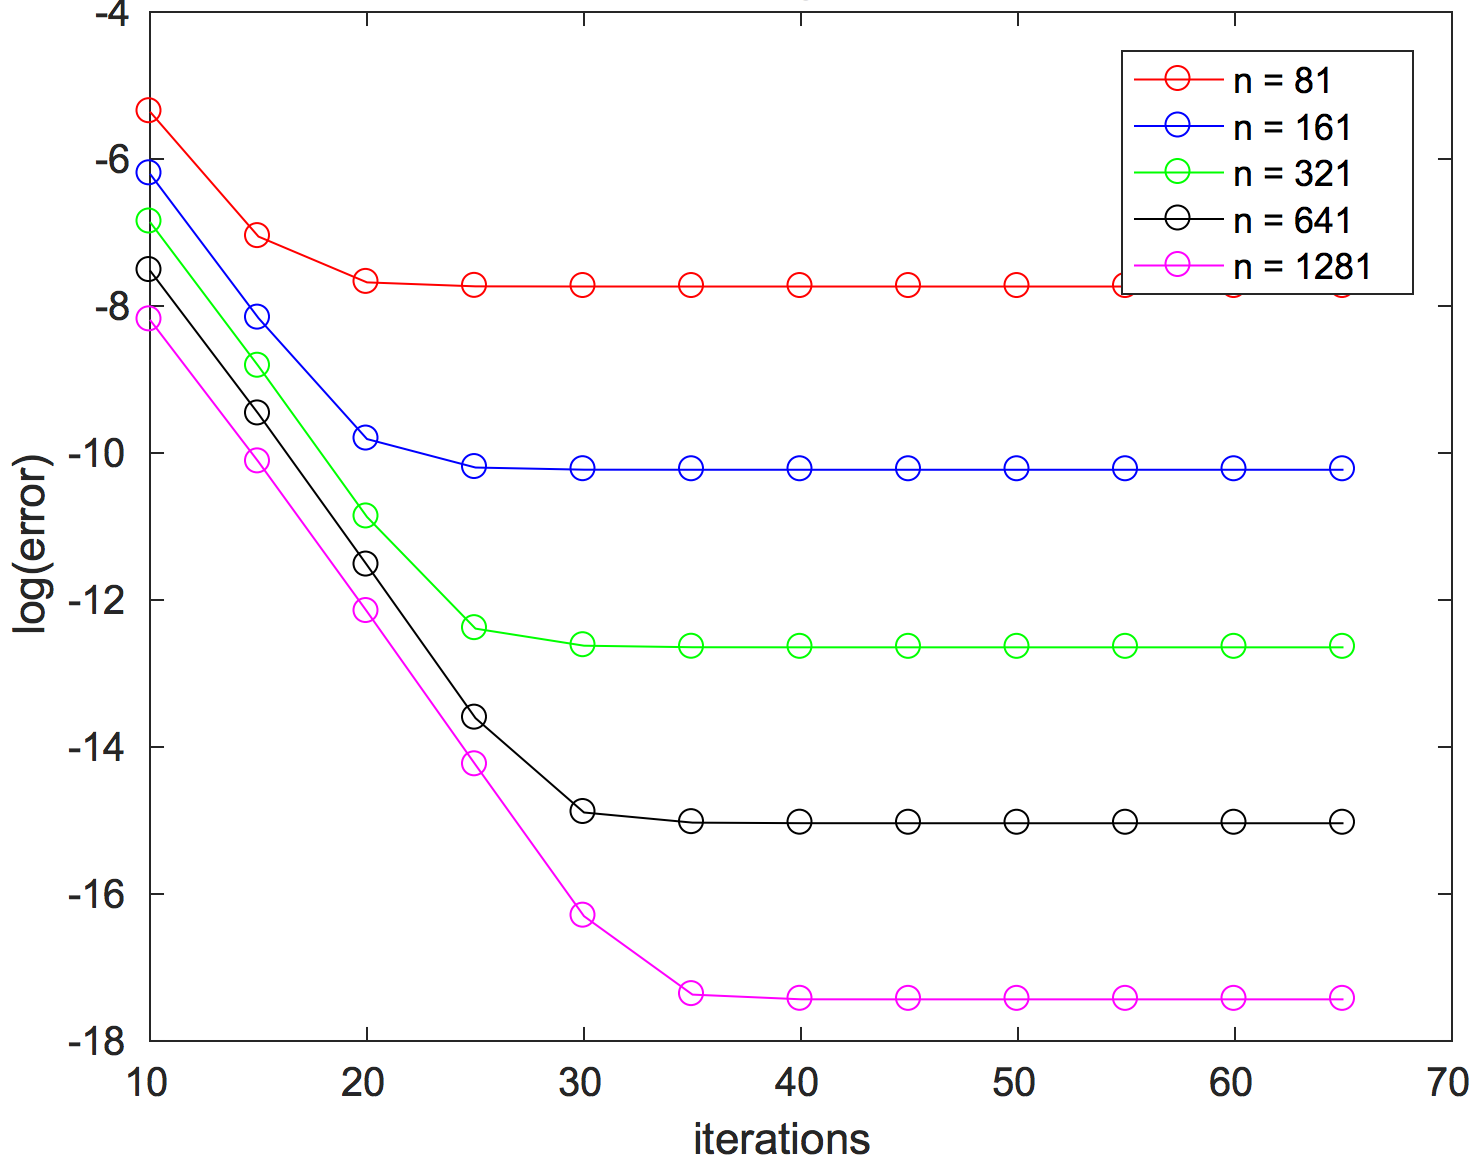
\includegraphics[width=.3\textwidth]{/Users/meganchang/Desktop/Thesis/images/Iterations_Flower_1.png}} \quad
\subfigure[Fat-Petal Flower $L^\infty$]{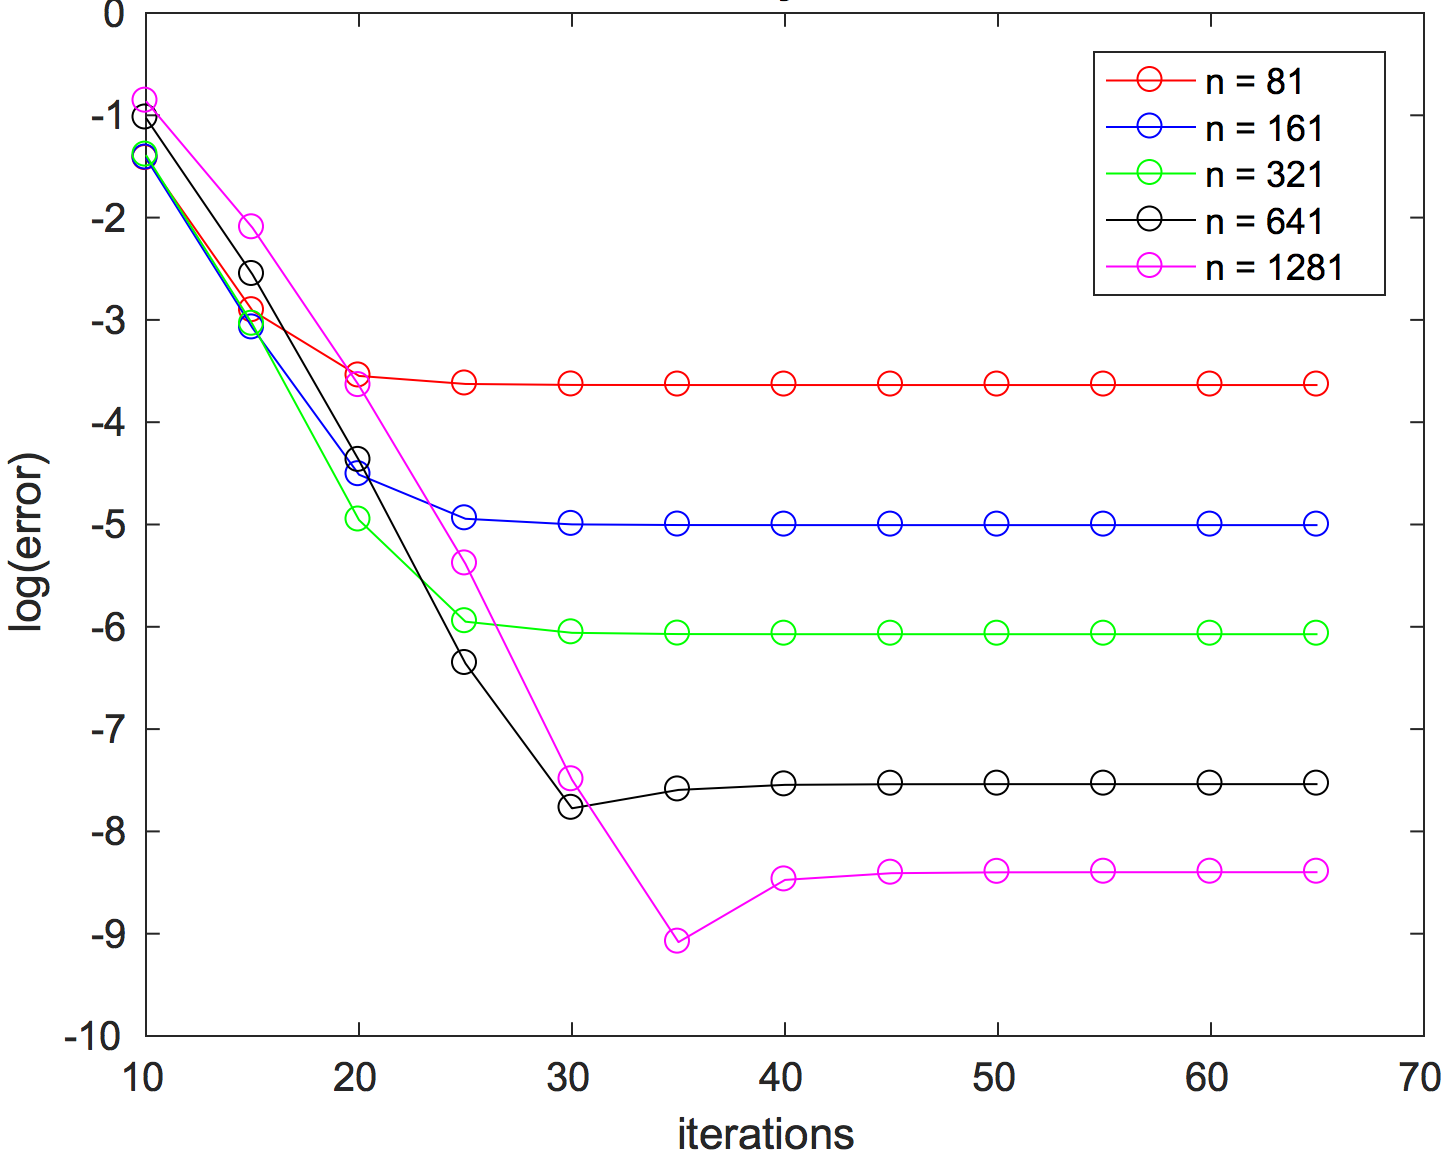
\includegraphics[width=.3\textwidth]{/Users/meganchang/Desktop/Thesis/images/Iterations_Flower_inf.png}}\\
\subfigure[Thin-Petal Flower $L^1$]{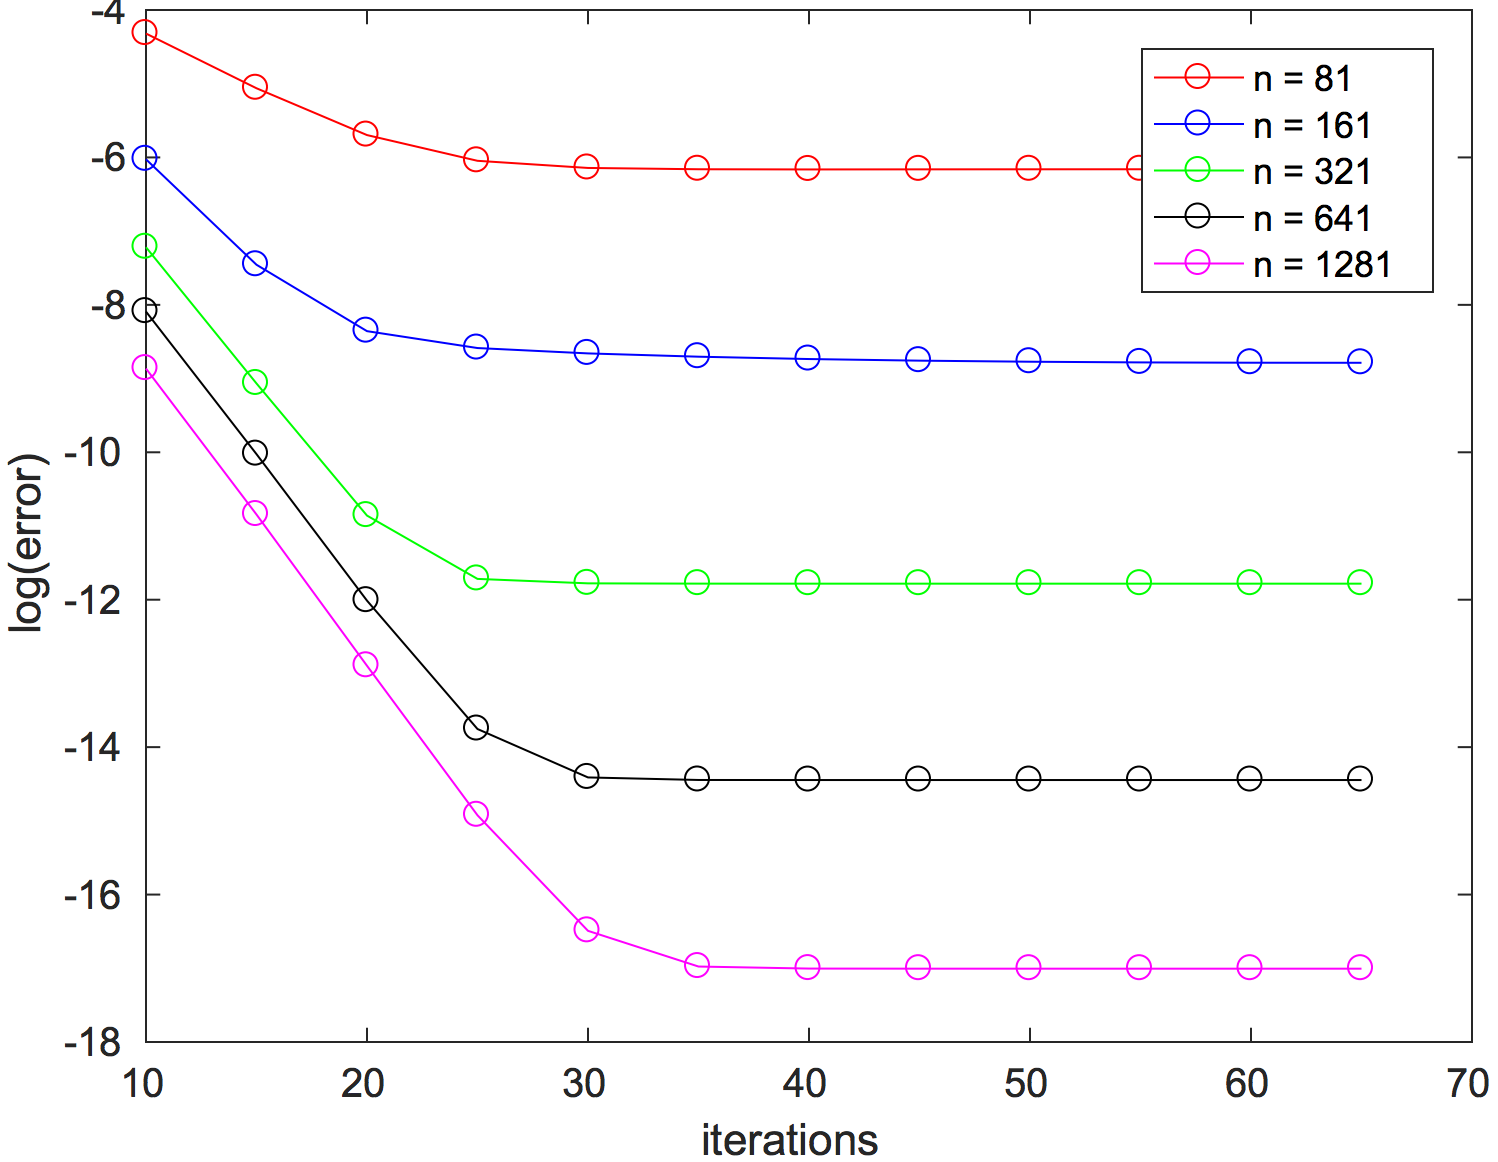
\includegraphics[width=.3\textwidth]{/Users/meganchang/Desktop/Thesis/images/Iterations_Crazy_1.png}} \quad
\subfigure[Thin-Petal Flower $L^\infty$]{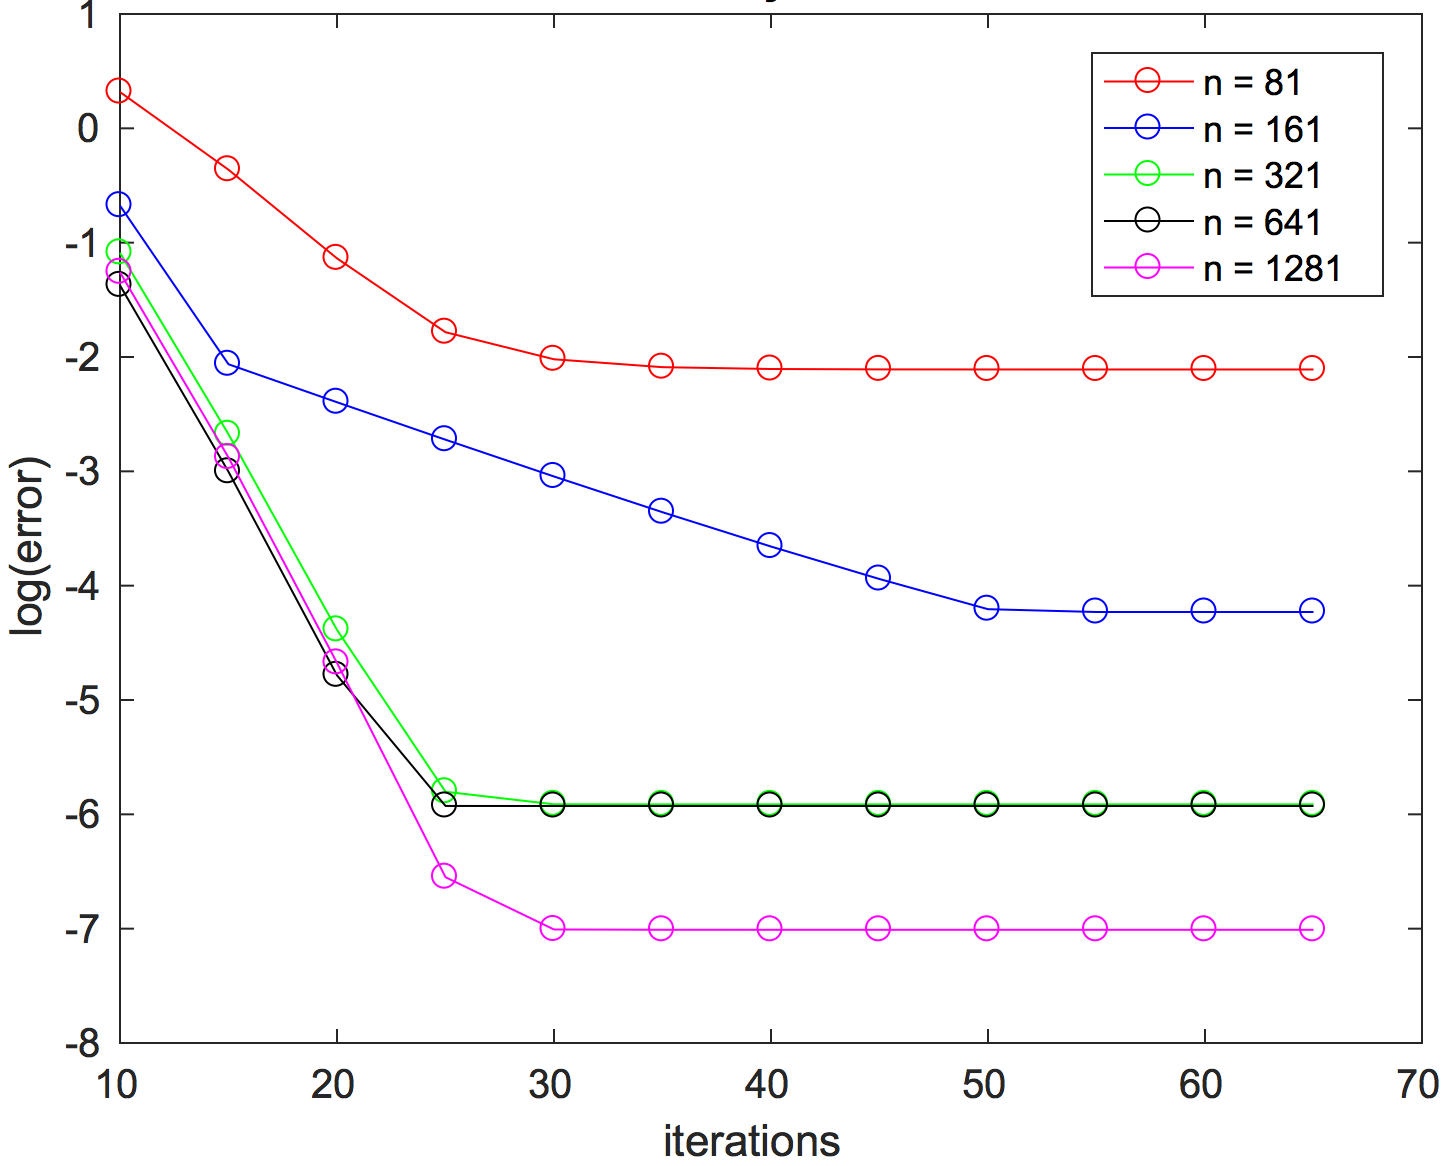
\includegraphics[width=.3\textwidth]{/Users/meganchang/Desktop/Thesis/images/Iterations_Crazy_inf.png}}\\
  \caption[Iterations to Reach Convergence for Third-Order Extrapolation]{Iterations required to reach convergence in the band of space $2 \Delta x$ outside the interface for the four level-set shapes described by in Table \ref{table:level_set_shapes}.}
  \label{fig:Third_Order_Iterations}
\end{figure}

As one can see in Figure \ref{fig:Third_Order_Iterations}, the accuracy continues to improve for a given number of iterations until steady state is reached. The necessary amount of iterations to achieve this maximum accuracy increases with the number of grid points.

The level-sets that displayed sharp features or kinks reached convergence faster than the smooth circle, but had much larger magnitudes of error at convergence. In Figure \ref{fig:Third_Order_Error_sharp}, one can see that this larger error is caused by the sharp corners. However, we found that for all level-set cases, 50 iterations was enough for convergence and so the following tables show orders of accuracy after 50 iterations, which we expect to have at least third-order convergence in $L^1$, and first-order convergence in $L^\infty$.


\begin{figure} [!h]
\centering
\subfigure[Diamond $L^1$]{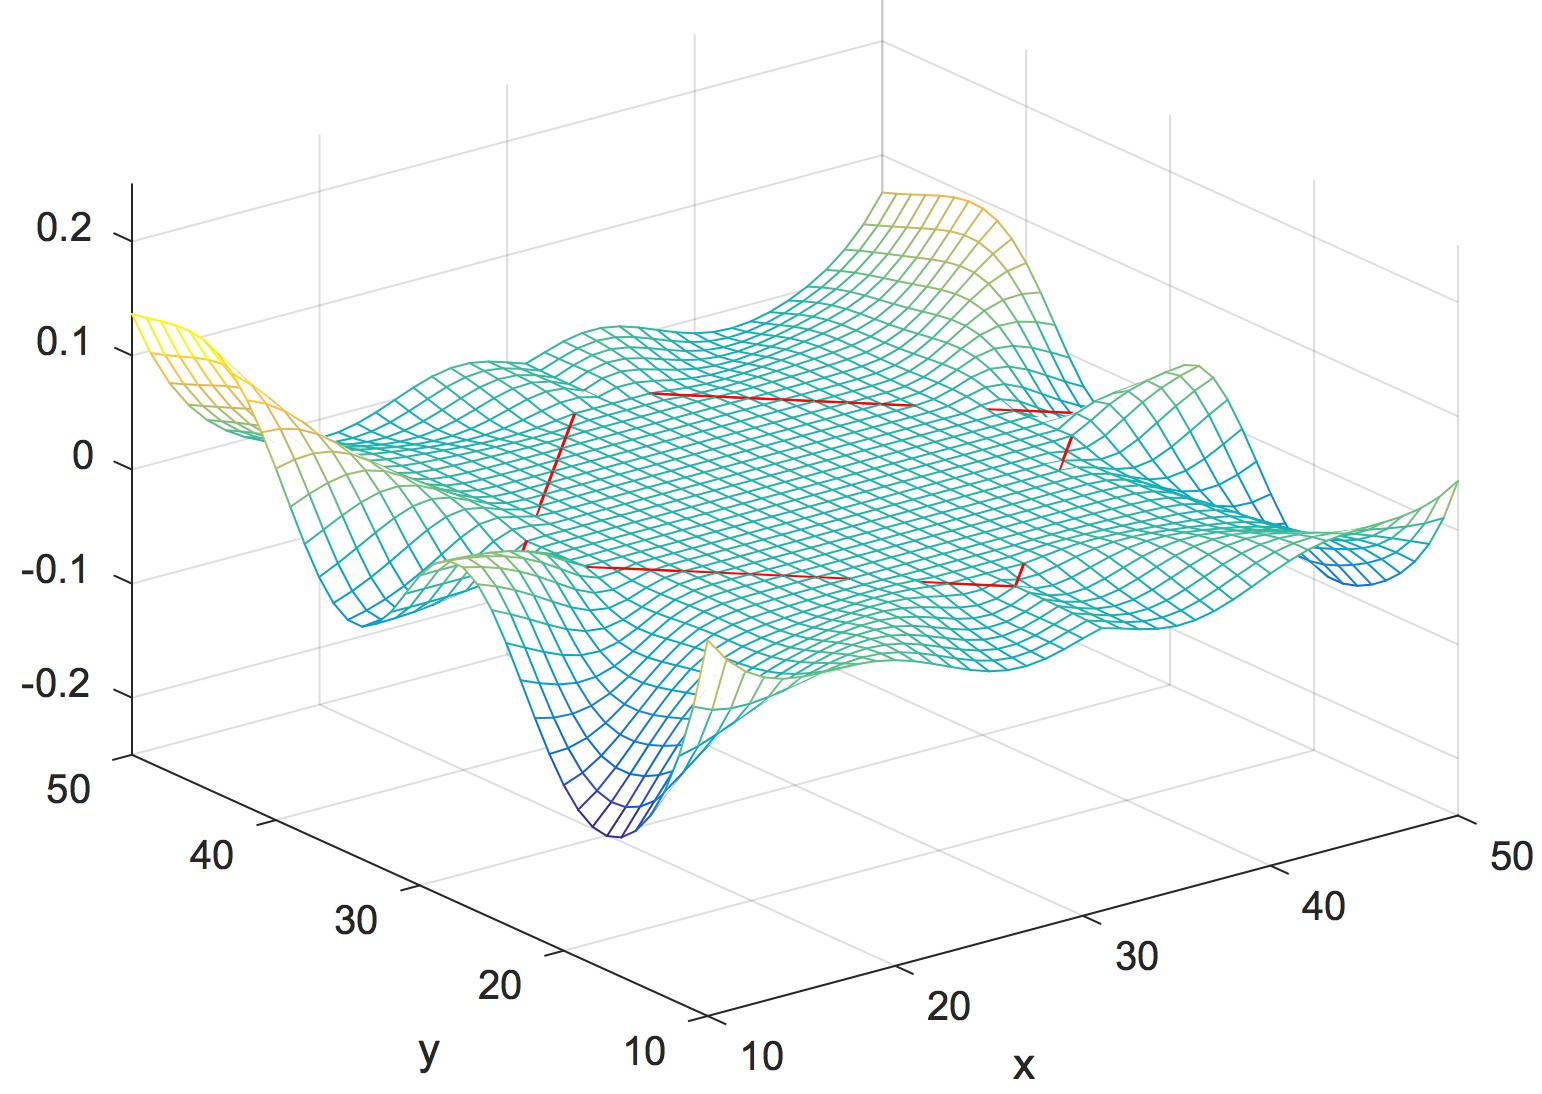
\includegraphics[width=.48\textwidth]{/Users/meganchang/Desktop/Thesis/images/Third_Order_Error_Plot_1.png}} \quad
\subfigure[Diamond $L^\infty$]{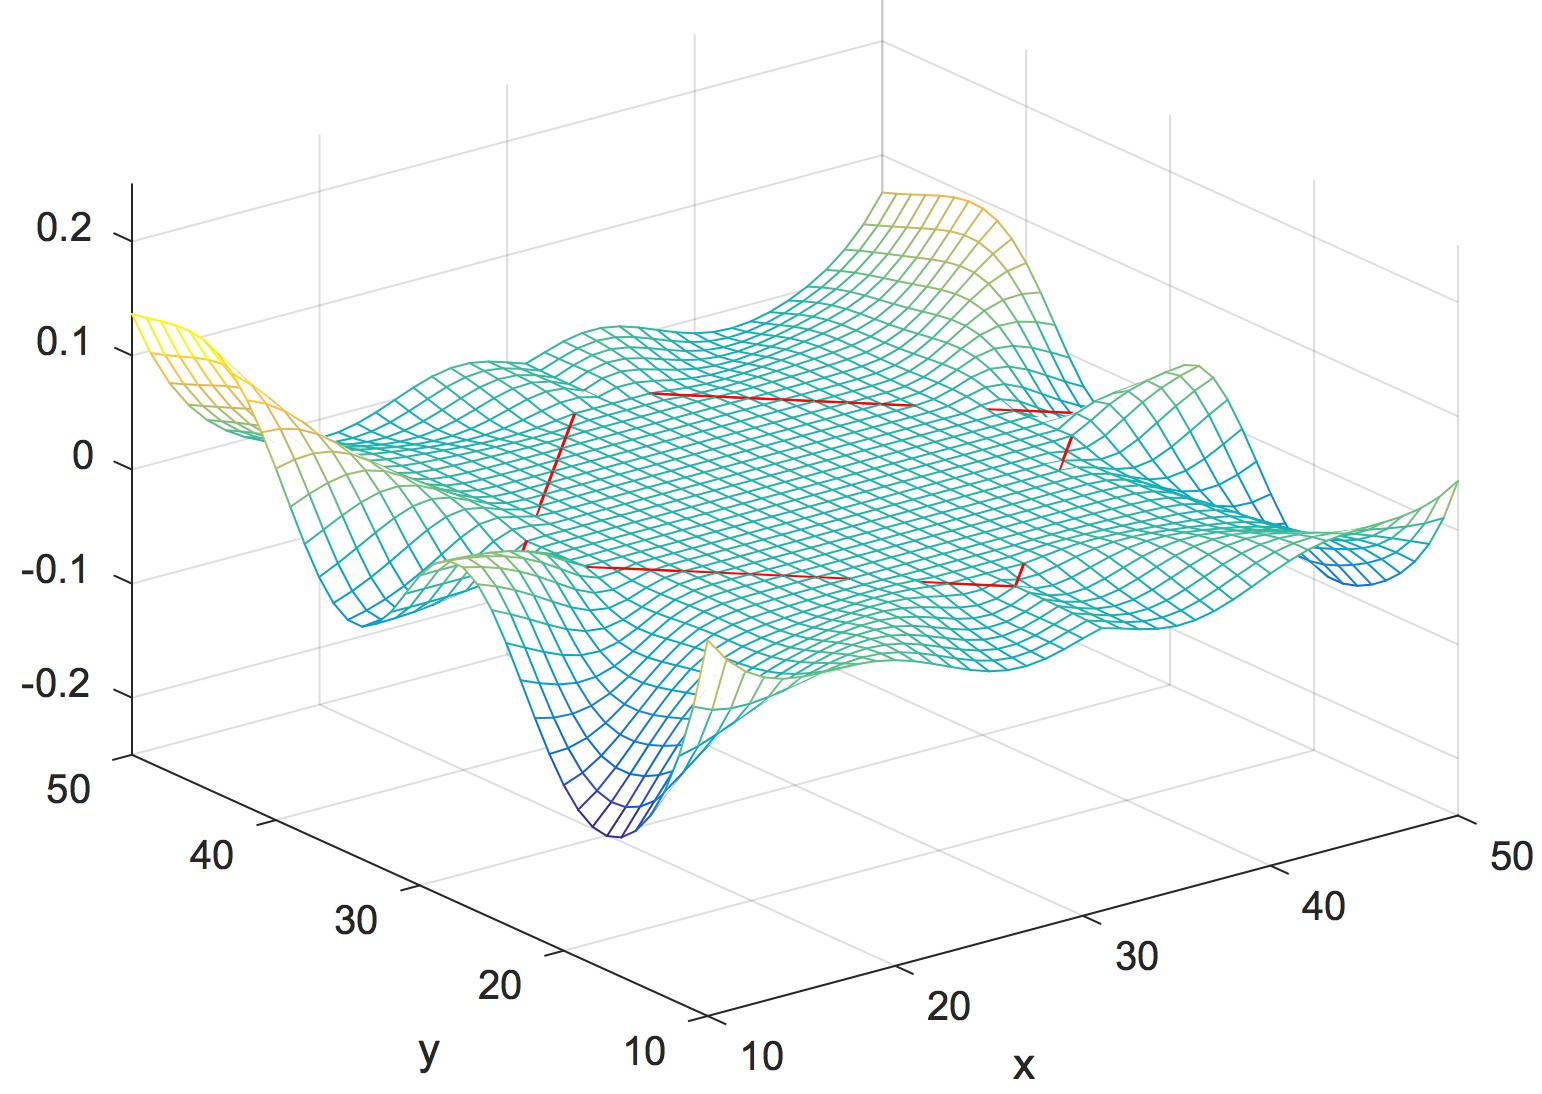
\includegraphics[width=.48\textwidth]{/Users/meganchang/Desktop/Thesis/images/Third_Order_Error_Plot_1.png}}\\
  \caption[Location of Error in Third-Order Extrapolation Method]{Notice the error arises at the sharp corners of the diamond level-set. Likewise, with the flower level-sets (not pictured), we observed the greatest error at the sharp corners where the petals meet at the base.}
  \label{fig:Third_Order_Error_sharp}
\end{figure}


\begin{table} [!h]
\caption{Circle Third-Order Extrapolation}
\centering
\begin{tabular}{c c c c c}
\hline
Grid Resolution & $L^1$ - error           & Order  & $L^{\infty}$ - error        & Order \\ \hline
81$\times$81     & $2.139 \times 10^{-5}$  &   -    & $2.757 \times 10^{-4}$  &  -    \\
161$\times$161   & $2.972 \times 10^{-6}$  &  2.84  & $9.393 \times 10^{-5}$   & 1.55  \\
321$\times$321   & $4.102 \times 10^{-7}$ &  2.86  & $2.707 \times 10^{-5}$   & 1.79  \\
\end{tabular}
\end{table}

\begin{table} [!h]
\caption{Diamond Third-Order Extrapolation}
\centering
\begin{tabular}{c c c c c}
\hline
Grid Resolution & $L^1$ - error           & Order  & $L^{\infty}$ - error        & Order \\ \hline
81$\times$81     & $2.459 \times 10^{-4} $ &   -    & $1.470 \times 10^{-2} $  &  -    \\
161$\times$161   & $3.157 \times 10^{-5} $ &  2.96  & $7.500 \times 10^{-3}$   & 0.97  \\
321$\times$321   & $4.014 \times 10^{-6} $ &  2.98  & $3.800 \times 10^{-3}$   & 0.98  \\
\end{tabular}
\end{table}

\begin{table} [!h]
\caption{Fat-Petal Flower Third-Order Extrapolation}
\centering
\begin{tabular}{c c c c c}
\hline
Grid Resolution & $L^1$ - error           & Order  & $L^{\infty}$ - error        & Order \\ \hline
81$\times$81     & $2.654 \times 10^{-4}$  &   -    & $1.410 \times 10^{-2}$   &  -  \\
161$\times$161   & $1.262 \times 10^{-5}$  &  4.39  & $4.900 \times 10^{-3}$   & 1.52\\
321$\times$321   & $1.147 \times 10^{-6}$ &  3.46  & $4.999 \times 10^{-4} $  & 3.30\\
\end{tabular}
\end{table}


\begin{table} [!h]
\caption{Thin-Petal Flower Third-Order Extrapolation}
\centering
\begin{tabular}{c c c c c}
\hline
Grid Resolution & $L^1$ - error           & Order  & $L^{\infty}$ - error        & Order \\ \hline
81$\times$81     & $1.370 \times 10^{-2}$  &   -    & $1.793 \times 10^{-1}   $ &  -    \\
161$\times$161   & $6.558 \times 10^{-4}$  &  4.38  & $5.070 \times 10^{-2}  $ & 1.82  \\
321$\times$321   & $1.590 \times 10^{-5}$  &  5.37  & $7.000 \times 10^{-3}$   & 2.85  \\
\end{tabular}
\end{table}

\section{Constant Extrapolation of the Interface Velocity}\label{section:constant_extrapolation}

Although we are interested only in the level-set velocity at the interface $\phi = 0$, we compute the level-set velocity on our entire grid. This means different parts of our level-set will be displaced at different rates which could lead to a poorly behaved level-set. However, there is a simple preconditioning tool we can use to make our level-set behave better and allow the reinitialization equation to converge faster. We implement constant extrapolation of the interface velocity. This is a first-order extrapolation method, and thus uses only one PDE with an imposed first derivative of 0
\begin{equation}  
\begin{aligned}
\frac{\partial v_x}{\partial \tau} + H(\phi,v_x)(\vec{n} \cdot \nabla v_x) = 0,\\
\frac{\partial v_y}{\partial \tau} + H(\phi,v_y)(\vec{n} \cdot \nabla v_y) = 0.\\
\end{aligned}
\end{equation}
We call this function using $\phi$ to constantly extrapolate the velocities from the interface into $\Omega^+$, then repeat the process using $-\phi$ to extrapolate the velocities from the interface into $\Omega^-$. In this way, the values at the interface will be extrapolated in the normal direction throughout the grid space. Figure \ref{fig:constant_extrapolation_1} demonstrates this constant extrapolation.
\begin{figure} [!h]
\centering
\subfigure[Velocity in the subdomain $\Omega^-$]{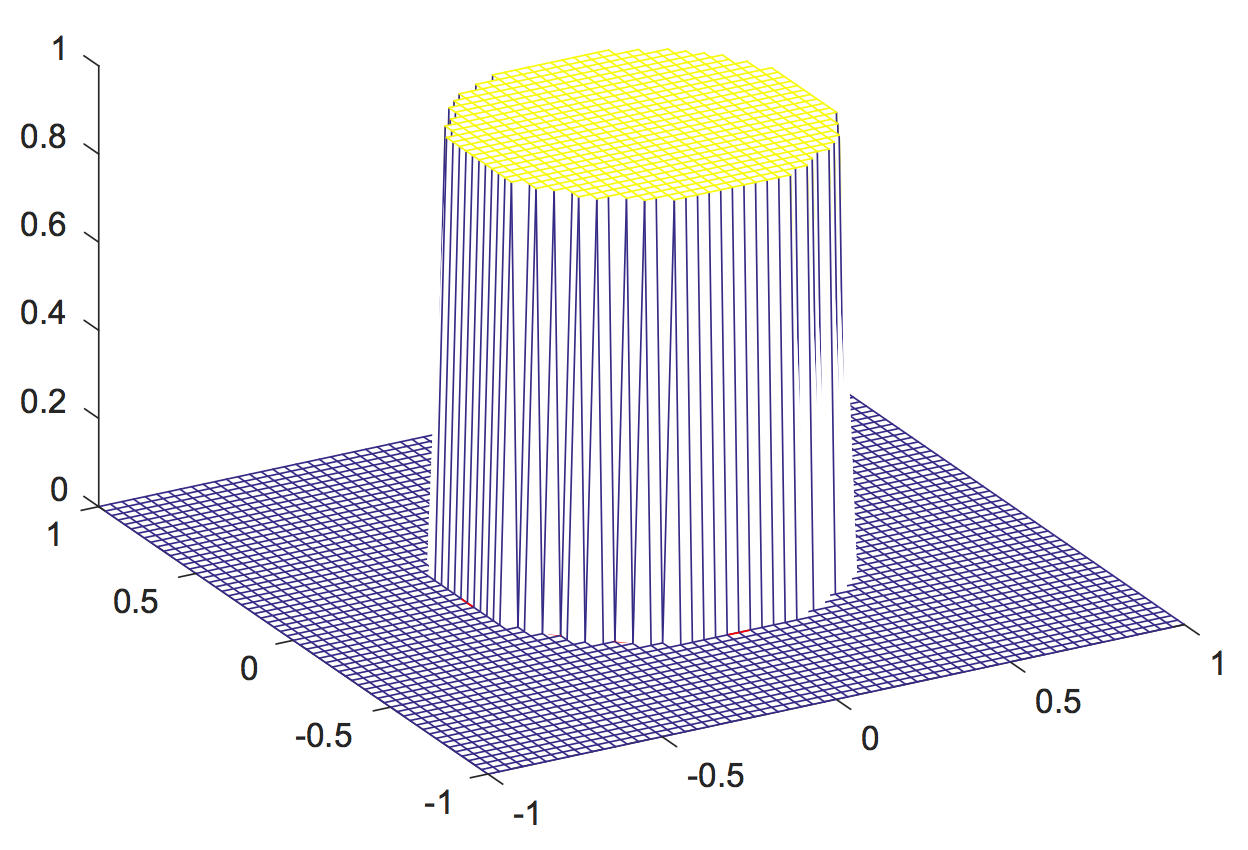
\includegraphics[width=.48\textwidth]{/Users/meganchang/Desktop/Thesis/images/Constant_Extrapolation_1.png}} \quad
\subfigure[Velocity extrapolated beyond the interface]{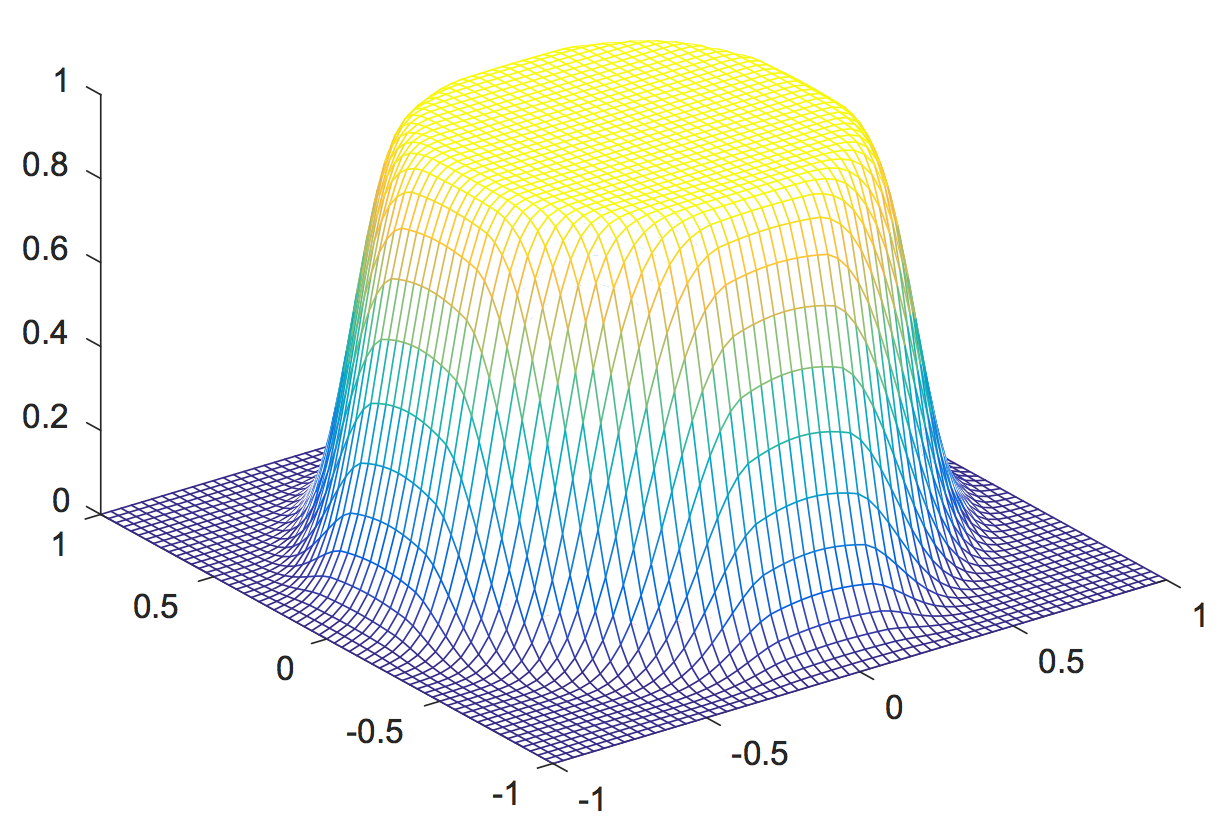
\includegraphics[width=.48\textwidth]{/Users/meganchang/Desktop/Thesis/images/Constant_Extrapolation_2.png}}
  \caption[Constant Extrapolation Method]{Constant normal extrapolation of the values in the $\Omega^-$ region out into the $\Omega^+$ region.}
  \label{fig:constant_extrapolation_1}
\end{figure}


%=== Chapter 5  ============================================
\chapter{Advection}

We use the level-set equation \eqref{eqn:level_set} to keep track of the moving interface. This equation can be described as advection, or the transport of material via bulk motion (see Figure \ref{fig:advection}). Advection is described by a linear hyperbolic PDE, which is not trivial to solve numerically. Because it contains strictly first derivatives and a causality principle, unique numerical challenges arise in its discretization. For instance, using standard central differencing techniques can create instability. Upwind schemes are a popular numerical technique used to tackle such problems because they consider the direction of propagation of information. However, we must be careful to select the appropriate time step to minimize both even-order spatial derivative related errors (i.e. numerical dissipation, or damping); and odd-order spatial derivative related errors (i.e. numerical dispersion, or the incorrect propagation velocity, which can also produce dispersive waves left in the wake). Choosing the appropriate CFL (Courant-Friedrichs-Lewy) number will reduce these errors as well as ensure numerical stability. In practice, we use a CFL number of 0.5.

\begin{figure} [!h]
\centering
\subfigure[Initial Data]{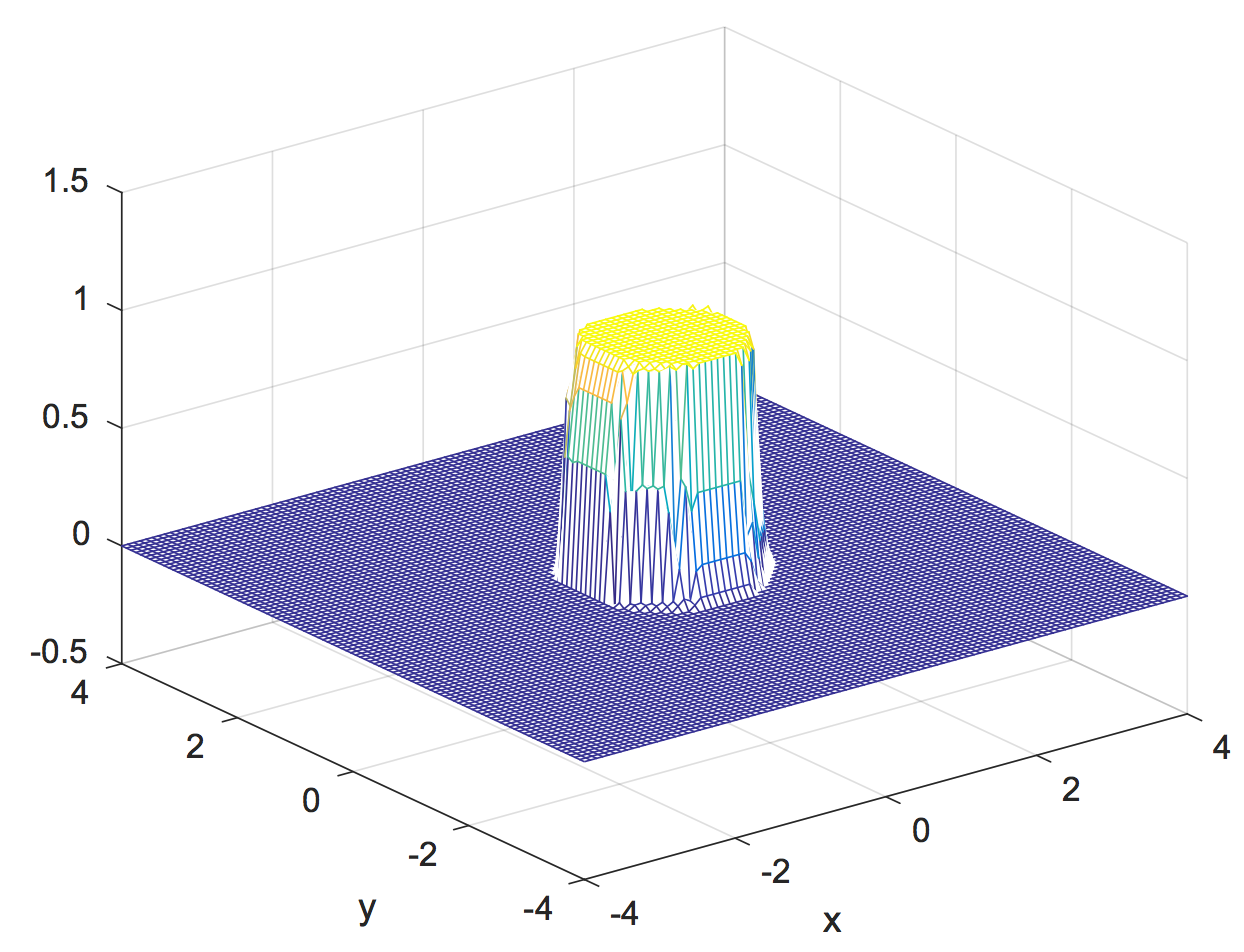
\includegraphics[width=.4\textwidth]{/Users/meganchang/Desktop/Thesis/images/Advection_00.png}}\\
\subfigure[$u = +1, v =+ 1$]{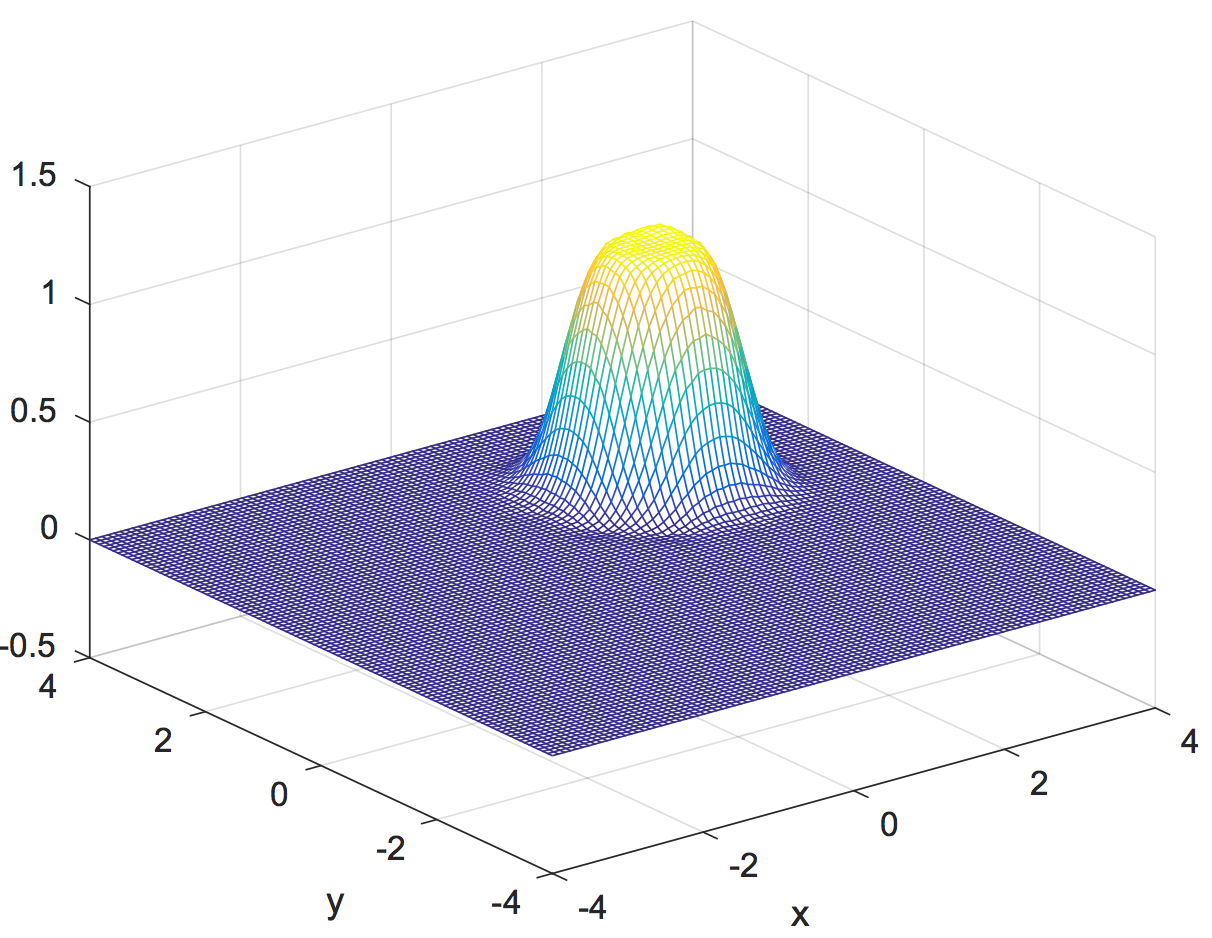
\includegraphics[width=.4\textwidth]{/Users/meganchang/Desktop/Thesis/images/Advection_01.png}} \quad
\subfigure[$u = +1, v = -1$]{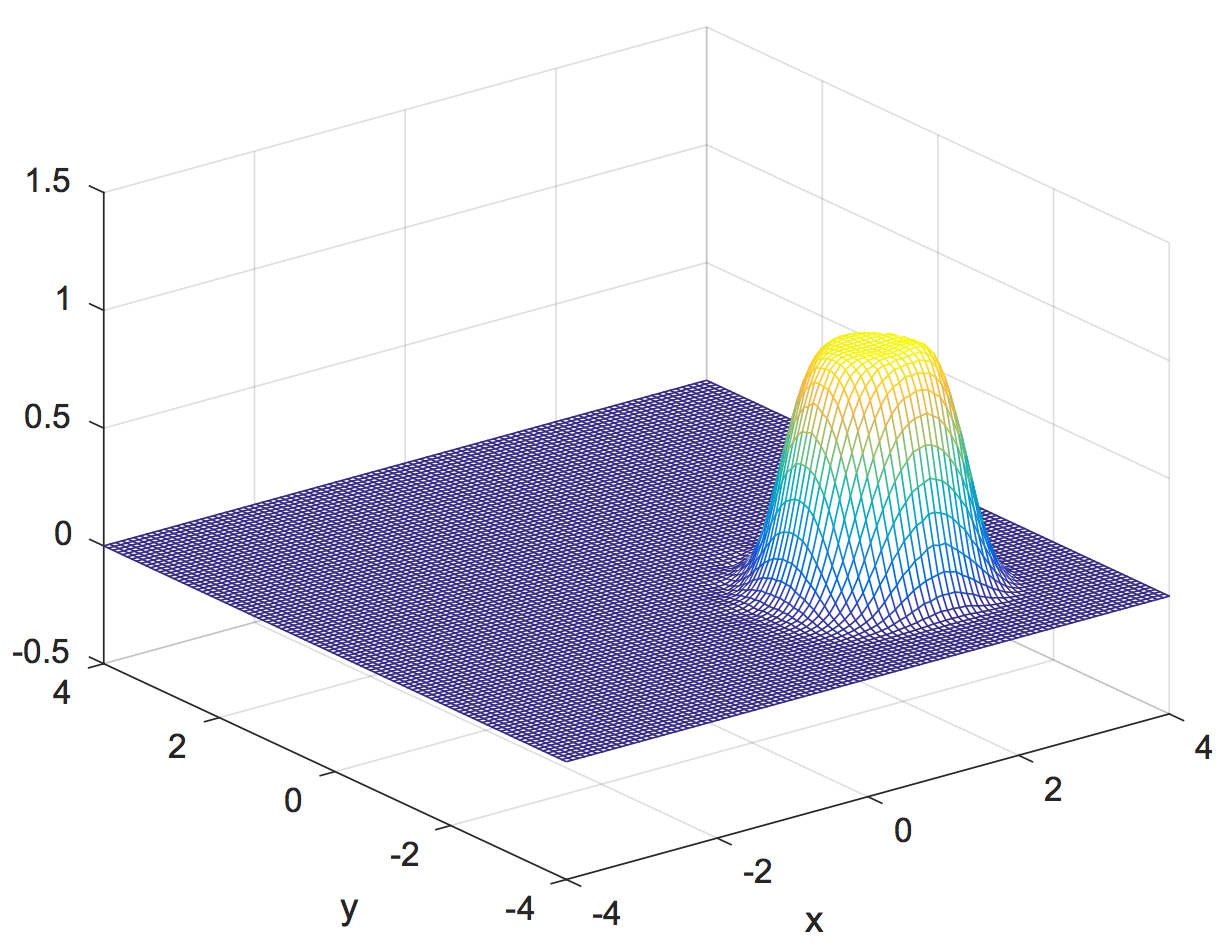
\includegraphics[width=.4\textwidth]{/Users/meganchang/Desktop/Thesis/images/Advection_02.png}}\\
\subfigure[$u = -1, v =+ 1$]{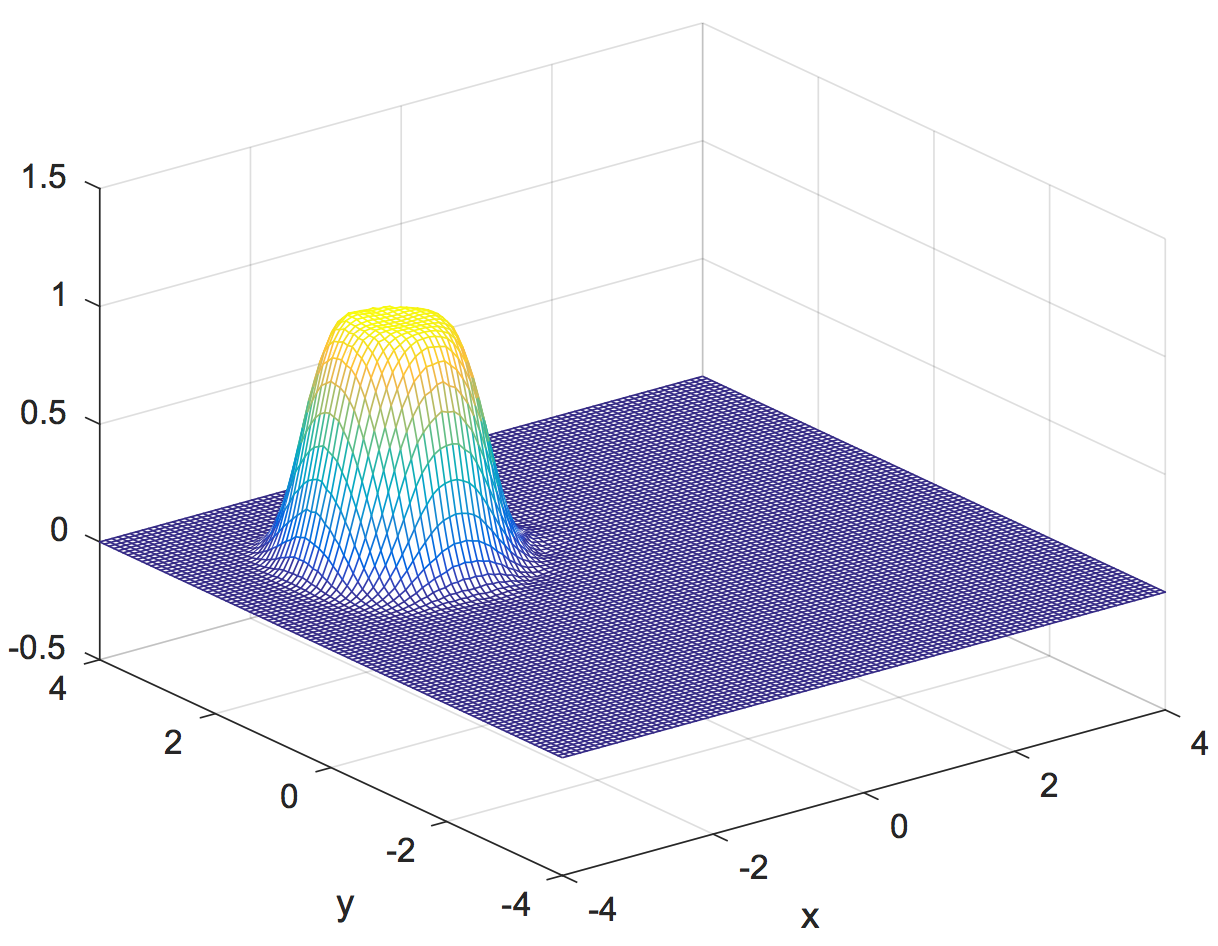
\includegraphics[width=.4\textwidth]{/Users/meganchang/Desktop/Thesis/images/Advection_03.png}} \quad
\subfigure[$u = -1, v = -1$]{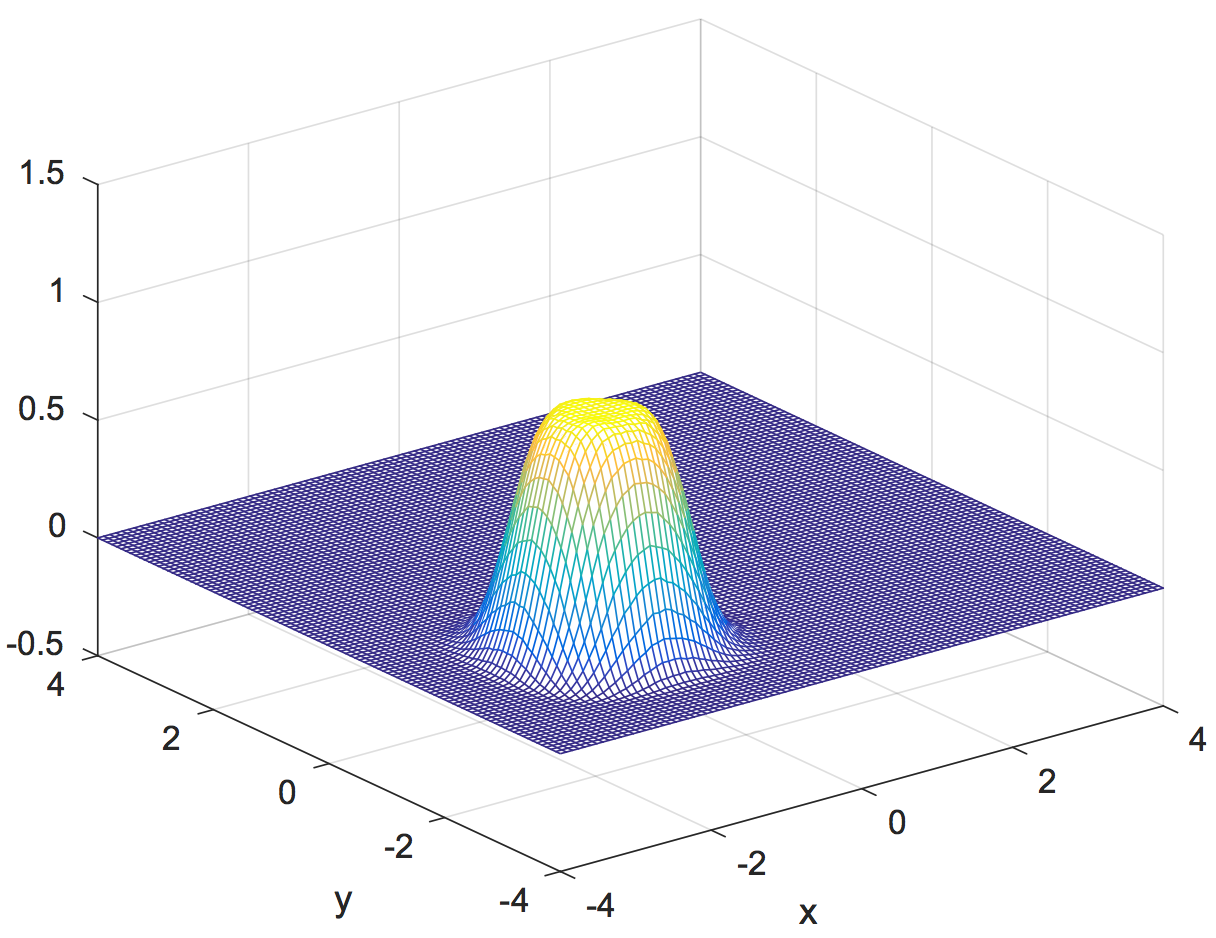
\includegraphics[width=.4\textwidth]{/Users/meganchang/Desktop/Thesis/images/Advection_04.png}}
  \caption[Advection]{Advection in different directions.}
  \label{fig:advection}
\end{figure}

Thus far, we have used first-order accurate upwind schemes which are impractical in this application. But, higher-order methods like the Lax-Wendroff and Beam-Warming methods produce oscillatory results near discontinuities. Thus, we develop a higher-order spatial discretization scheme known as WENO, or the Weighted Essentially Non-Oscillatory scheme, first introduced by Liu, Osher, and Chan in [6]. We combine this with a TVD RK3 time discretization to compute advection.

\section{WENO Schemes}  \label{section:WENO}
The WENO scheme was developed for solving one-sided finite difference problems with higher-order accuracy in smooth regions, while simultaneously improving behavior near discontinuities. This is achieved by considering three different stencils (depending on the upwind direction), and determining for each grid point which stencil or convex weighted combination of stencils will produce the smoothest results.

Figure \ref{fig:WENO_choice}(a) shows the three substencil choices for the upwind direction $D_{x}^{+}$, so called because it involves the points $i+1$ and $i$, such that information propagates from $i+1$ to $i$ and $v_x < 0$. Figure \ref{fig:WENO_choice}(b) shows the three substencil choices for the upwind direction $D_{x}^{-}$, so called because it involves the points $i-1$ and $i$, such that information propagates from $i-1$ to $i$ and $v_x > 0$. 

\begin{figure} [!h]
\centering
\subfigure[Possible stencil choices for computing $D_{x}^{+}$]{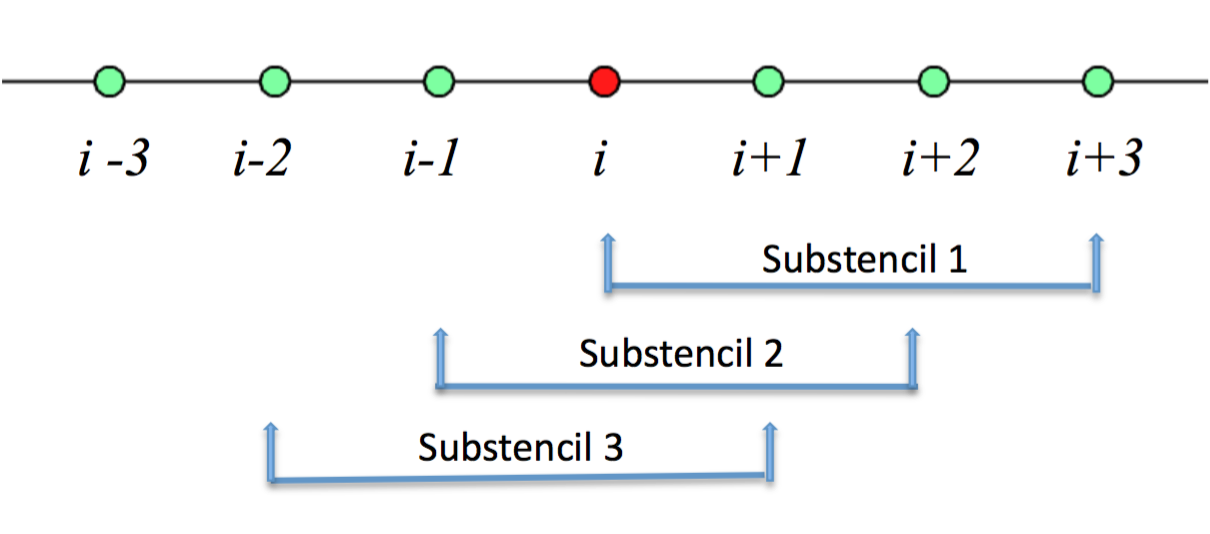
\includegraphics[width=.44\textwidth]{/Users/meganchang/Desktop/Thesis/images/Dxplus}} \\
\subfigure[Possible stencil choices for computing $D_{x}^{-}$]{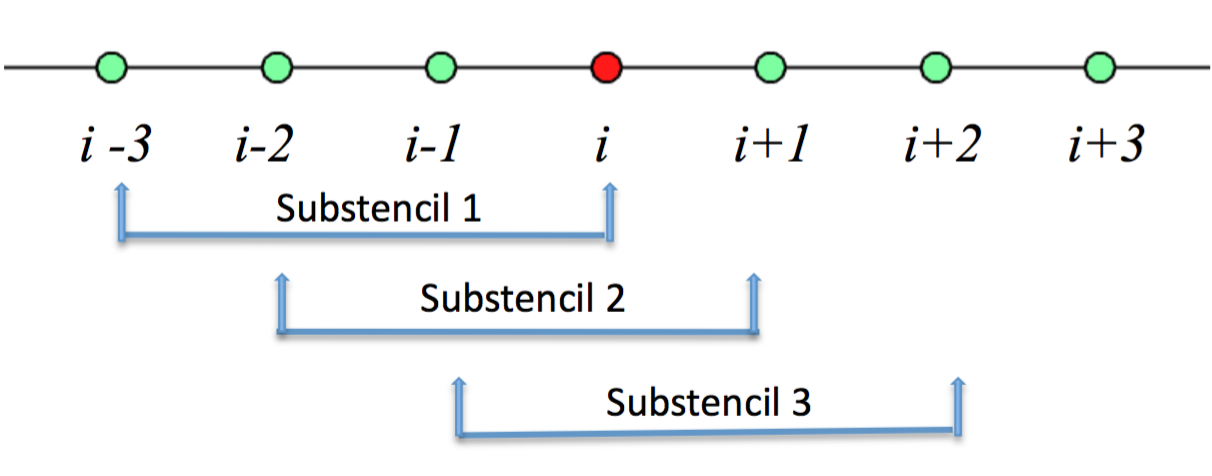
\includegraphics[width=.44\textwidth]{/Users/meganchang/Desktop/Thesis/images/Dxminus}}\\
    \caption[WENO Substencil Choices for Computing One-Sided Finite Differences]{WENO substencil choices for computing one-sided finite differences.}
  \label{fig:WENO_choice}
\end{figure}
Figure \ref{fig:WENO_example} shows an example of how we would choose the smoothest possible stencil.

\begin{figure} [!h]
\centering
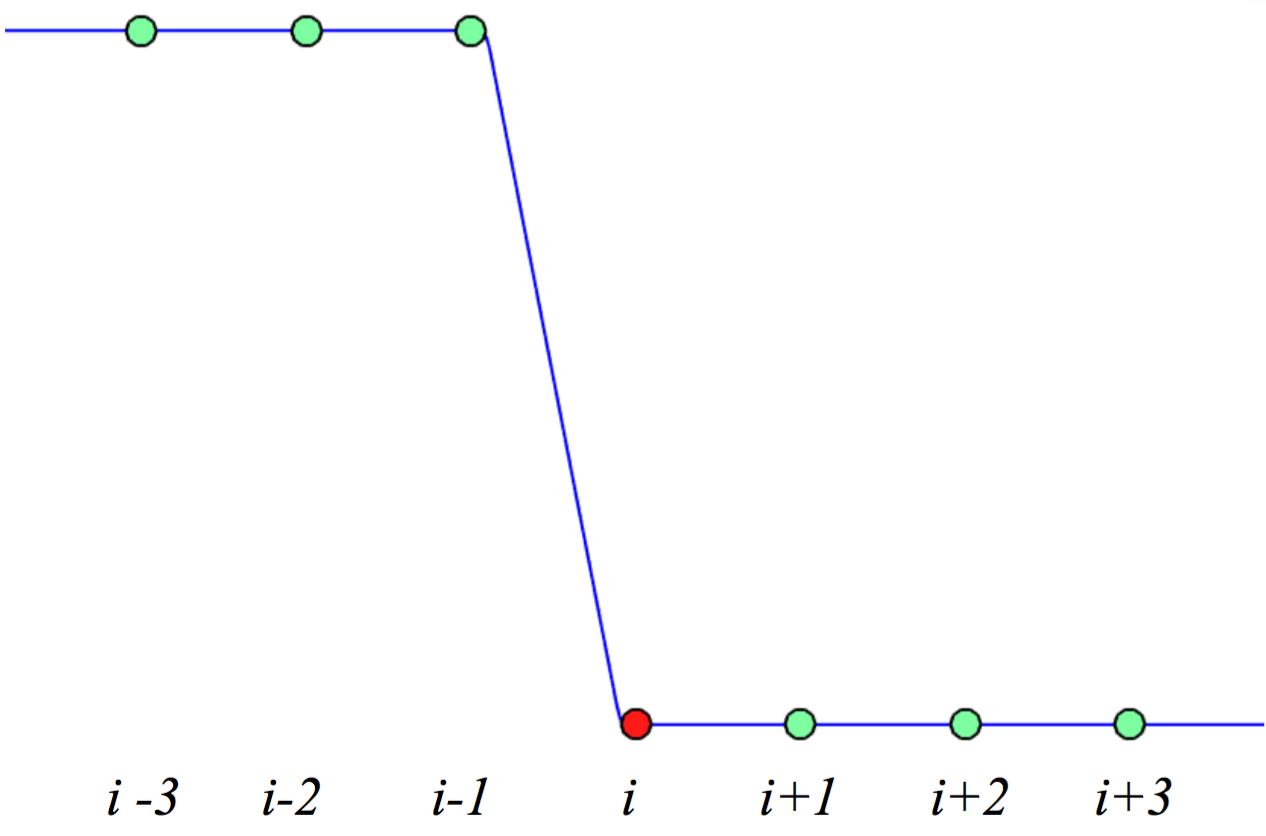
\includegraphics[width=.48\textwidth]{/Users/meganchang/Desktop/Thesis/images/WENO}
    \caption[WENO Substencil Selection Example]{Suppose for the stencil you see here, $v_x$ is negative, so that information is traveling from $i+1$ to $i$. We would then make our substencil selection from the options for $D_{x}^{+}$ in Figure \ref{fig:WENO_choice}(a). It is clear from inspection that substencils 2 and 3 introduce a new maximum which would trigger oscillations in the solution. Thus, we would ultimately choose substencil 1 because it is the smoothest.}
  \label{fig:WENO_example}
\end{figure}

This smoothness can be computed by determining the divided differences which measure the level of discontinuity in a solution. The three possible ENO approximations of $D_x^- u$ are
\begin{eqnarray*}
u_{x}^{1}&=&  \frac{d_{1}}{3}-\frac{7d_{2}}{6}+\frac{11d_{3}}{6}, \\
u_{x}^{2}&=& -\frac{d_{2}}{6}+\frac{5d_{3}}{6}+\frac{d_{4}}{3}, \\
u_{x}^{3}&=&  \frac{d_{3}}{3}+\frac{5d_{4}}{6}-\frac{d_{5}}{6},
\end{eqnarray*}
where $d_{k}$ is defined as the simple finite differences:
\begin{eqnarray*}
d_{1}=\frac{u_{i-2}-u_{i-3}}{\Delta x}, \\
d_{2}=\frac{u_{i-1}-u_{i-2}}{\Delta x}, \\
d_{3}=\frac{u_{i\>\>\>\>\>}-u_{i-1}}{\Delta x}, \\
d_{4}=\frac{u_{i+1}-u_{i\>\>\>\>\>}}{\Delta x}, \\
d_{5}=\frac{u_{i+2}-u_{i+1}}{\Delta x}.
\end{eqnarray*}
The WENO approximation of $D_x^- u$ is
\begin{eqnarray}
D^{-}_{x}u=\omega_{1}u_{x}^{1}+\omega_{2}u_{x}^{2}+\omega_{3}u_{x}^{3}, \label{eqn:WENO}
\end{eqnarray}
where the stencil weights $\omega$ create a convex combination (i.e. $\omega_1 + \omega_2 + \omega_3 = 1$), chosen to create fifth-order accuracy in regions of smoothness, and reduce oscillatory behavior near discontinuities. To begin, we calculate the smoothness $S$ of each stencil
\begin{eqnarray*}
S_{1}&=&\frac{13}{12}(d_{1}-2d_{2}+d_{3})^{2}+\frac14(d_{1}-4d_{2}+3d_{3})^{2}, \\
S_{2}&=&\frac{13}{12}(d_{2}-2d_{3}+d_{4})^{2}+\frac14(d_{2}-d_{4})^{2}, \\
S_{3}&=&\frac{13}{12}(d_{3}-2d_{4}+d_{5})^{2}+\frac14(3d_{3}-4d_{4}+d_{5})^{2}.
\end{eqnarray*}
Then, we define the coefficients $\alpha_{k}$ as
\begin{equation*}
\alpha_{1}=\frac{0.1}{(S_{1}+\epsilon)^{2}}, \quad
\alpha_{2}=\frac{0.6}{(S_{2}+\epsilon)^{2}}, \quad
\alpha_{3}=\frac{0.3}{(S_{3}+\epsilon)^{2}},
\end{equation*}
where $\epsilon=10^{-6} \times \max(d_{1}^{2}, d_{2}^{2}, d_{3}^{2}, d_{4}^{2}, d_{5}^{2})+10^{-99}$. Finally, we can compute $\omega_k$ as
\begin{equation*}
\omega_{1}=\frac{\alpha_{1}}{\alpha_{1}+\alpha_{2}+\alpha_{3}}, \quad
\omega_{2}=\frac{\alpha_{2}}{\alpha_{1}+\alpha_{2}+\alpha_{3}}, \quad
\omega_{3}=\frac{\alpha_{3}}{\alpha_{1}+\alpha_{2}+\alpha_{3}}.
\end{equation*}
The construction of $D^{+}_{x}u$ uses the same process, except that our simple finite differences $d_{k}$ change to
\begin{eqnarray*}
d_{1}=\frac{u_{i+3}-u_{i+2}}{\Delta x}, \\
d_{2}=\frac{u_{i+2}-u_{i+1}}{\Delta x}, \\
d_{3}=\frac{u_{i+1}-u_{i\>\>\>\>\>}}{\Delta x}, \\
d_{4}=\frac{u_{i\>\>\>\>\>}-u_{i-1}}{\Delta x}, \\
d_{5}=\frac{u_{i-1}-u_{i-2}}{\Delta x}.
\end{eqnarray*}

Further, to extend these schemes to two-dimensions, we simply execute the above dimension by dimension. That is to say, we begin with column $j = 1$, and complete the spatial discretization for this column before moving to the next column, $j = 2$. And to construct $D_y^+u$ and $D_y^-u$, we simply replace the $i$ index with $j$.

\section{Accuracy of WENO Schemes for Computing First Derivatives}

To test for the accuracy of our WENO schemes, we first used a continuous test function
\begin{equation}
\begin{aligned}
\phi(x,y)   &=  \cos(x)\sin(y),
\end{aligned}
\end{equation}
and solved analytically for the partial derivatives with respect to $x$ and $y$
\begin{equation} \label{eqn:analytical solution to phi_x}
\begin{aligned}
\phi_x(x,y) &=       -\sin(x)\sin(y), \\
\phi_y(x,y) &=  \>\>\>\cos(x)\cos(y),
\end{aligned}
\end{equation}
in the domain $\Omega$ = [0,2$\pi$]$^2$ so that periodic boundary conditions could be applied (for the sake of error analysis). We compare $\phi_x$ to the resulting numerical solution found using our $D_x^+$ and $D_x^-$ schemes; and compare $\phi_y$ to the numerical solution found using $D_y^+$ and $D_y^-$. For a continuous function like this, we expect fifth-order accuracy, and from Table \ref{table:WENO_continuous}, we can see that this was indeed achieved. The $L^1$ and $L^\infty$ error, as well as the orders were the same for all four upwind directions. 

\begin{table} [!h]
\caption{2D WENO Scheme for All Upwind Directions}
\label{table:WENO_continuous}
\centering
\begin{tabular}{c c c c c}
\hline
Grid Resolution  & $L^1$ - error    & Order  & $L^\infty$ - error & Order \\ \hline
81$\times$81          & $5.502 \times 10^{-6} $ &   -    & $3.489 \times 10^{-7}$   &  -  \\
161$\times$161        & $1.738 \times 10^{-7}$  &  4.98  & $1.090 \times 10^{-8} $  & 5.00\\
321$\times$321        & $5.426 \times 10^{-9}$  &  5.00  & $3.405 \times 10^{-10} $ & 5.00\\
\end{tabular}
\end{table}


Perhaps, of more interest is what happens when we use a discontinuous function. For this second test, we used the piecewise function shown in Figure \ref{fig:discontinuous_WENO} and defined by
\begin{equation}
\begin{aligned}
    \phi(x,y) \>  = 
\begin{cases}
    \>\>\>\cos(x)\sin(y) & \text{for   }\>\>\>\>\>\>\>\>\> 0 \le x < N/3, \\ 
    -\cos(x)\sin(y) & \text{for   }\>\>\>N/3 \le x \le 2N/3, \\
    \>\>\>\cos(x)\sin(y) & \text{for   }\>2N/3 < x \le N,
\end{cases}
\end{aligned}
\end{equation}
where $N$ is the number of points in the grid, so that the function is the same in the initial and final third, but negative in the middle third. By beginning and ending with the same function, we can impose periodic boundary conditions which was necessary for accuracy testing. The above equation is discontinuous in the $x$-direction, and so was used to test our $D_x^+$ and $D_x^-$ programs against the exact analytical solution $\phi_x$ in \eqref{eqn:analytical solution to phi_x}. Again, noting that for the middle third, we use $- \phi_x$ \eqref{eqn:analytical solution to phi_x}. We use the same process to test the accuracy of $D_y^+$ and $D_y^-$, except that we make our function discontinuous along $y$, instead:
\begin{equation}
\begin{aligned}
    \phi(x,y) \>  = 
\begin{cases}
    \>\>\>\cos(x)\sin(y) & \text{for   }\>\>\>\>\>\>\>\>\> 0 \le y < N/3, \\ 
    -\cos(x)\sin(y) & \text{for   }\>\>\>N/3 \le y \le 2N/3, \\
    \>\>\>\cos(x)\sin(y) & \text{for   }\>2N/3 < y \le N.
\end{cases}
\end{aligned}
\end{equation}

For a discontinuous function, the greatest error in our WENO scheme accumulates near the discontinuity with a peak of error along the row or column at which the discontinuity actually occurs. Neglecting this one row of error which is impossible to avoid, we would expect at least third-order convergence for our piecewise function. Tables \ref{table:2D_WENO_1} - \ref{table:2D_WENO_4} show that for each of the four one-sided finite difference WENO scheme, third-order accuracy is achieved.

\begin{figure} [!h]
\centering
\subfigure[Mesh: Discontinuous function $\phi$ about $x$]{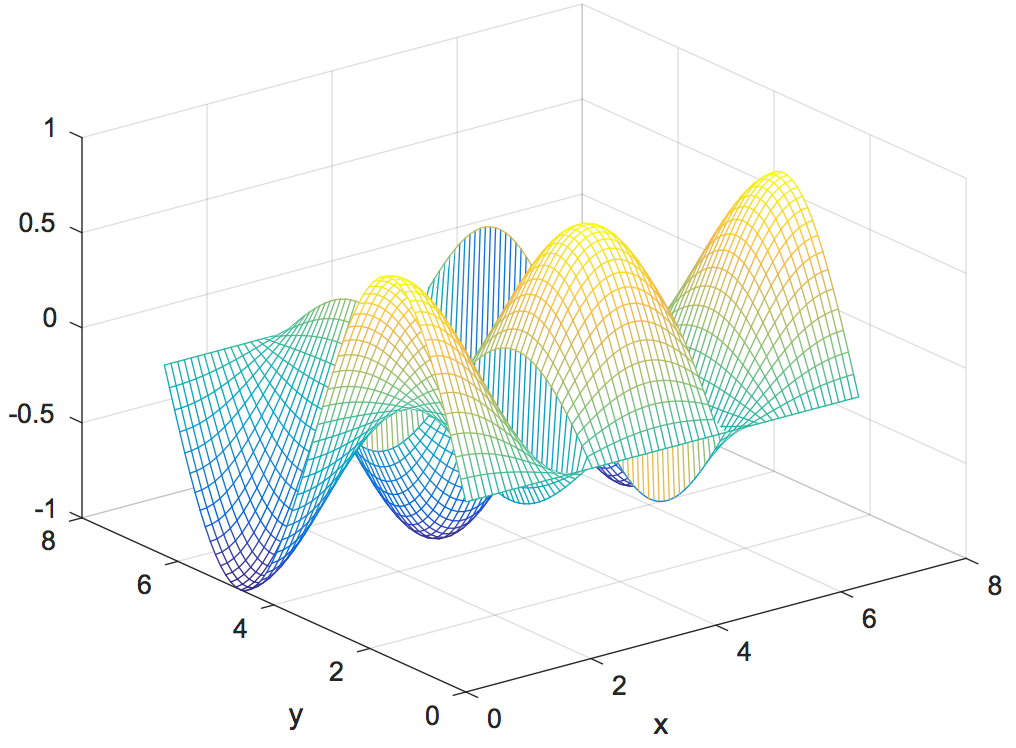
\includegraphics[width=.48\textwidth]{/Users/meganchang/Desktop/Thesis/images/Discontinuous_x.png}} \quad
\subfigure[Contour: Discontinuous function $\phi$ about $x$]{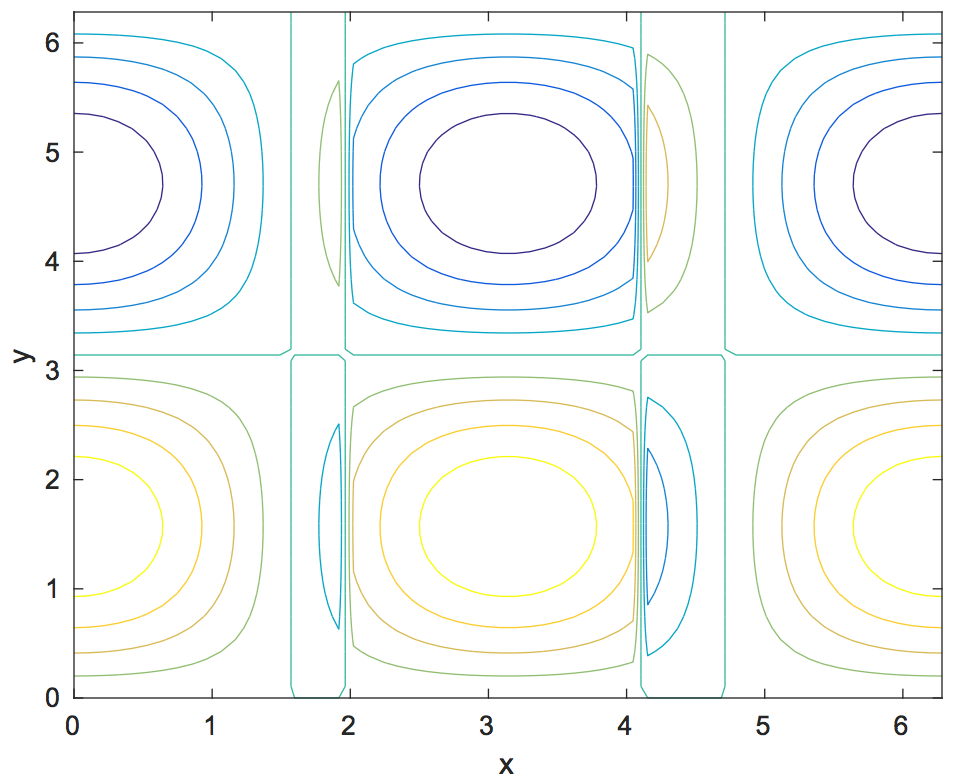
\includegraphics[width=.48\textwidth]{/Users/meganchang/Desktop/Thesis/images/Discontinuous_x_contour.png}} \\
\subfigure[Mesh: Discontinuous function $\phi$ about $y$]{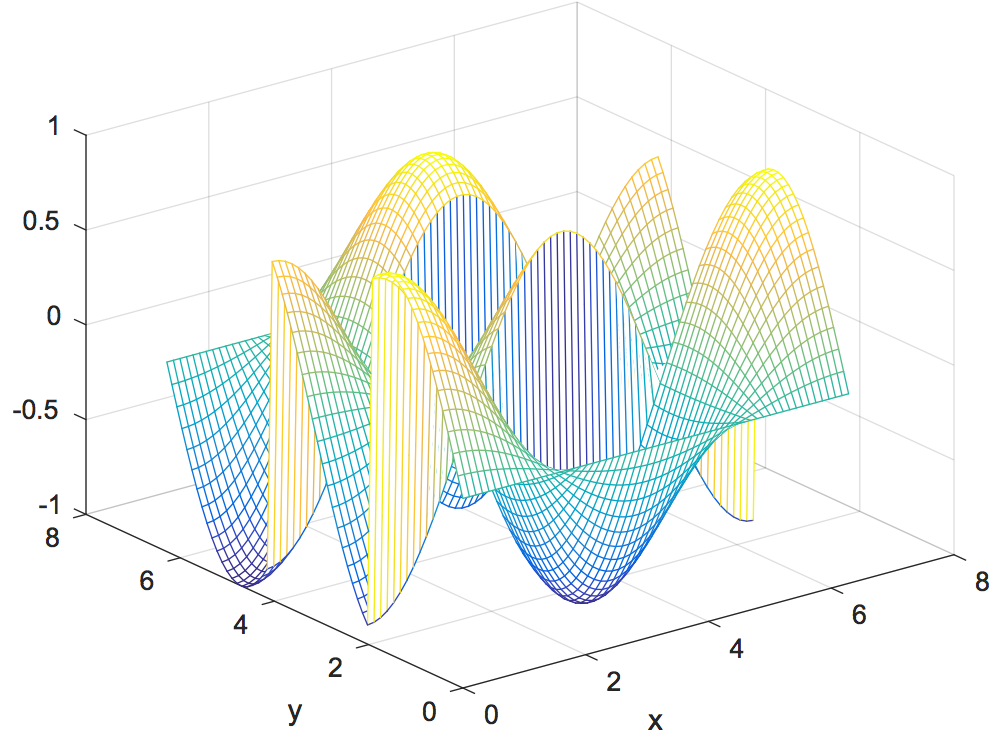
\includegraphics[width=.48\textwidth]{/Users/meganchang/Desktop/Thesis/images/Discontinuous_y.png}} \quad
\subfigure[Contour: Discontinuous function $\phi$ about $y$]{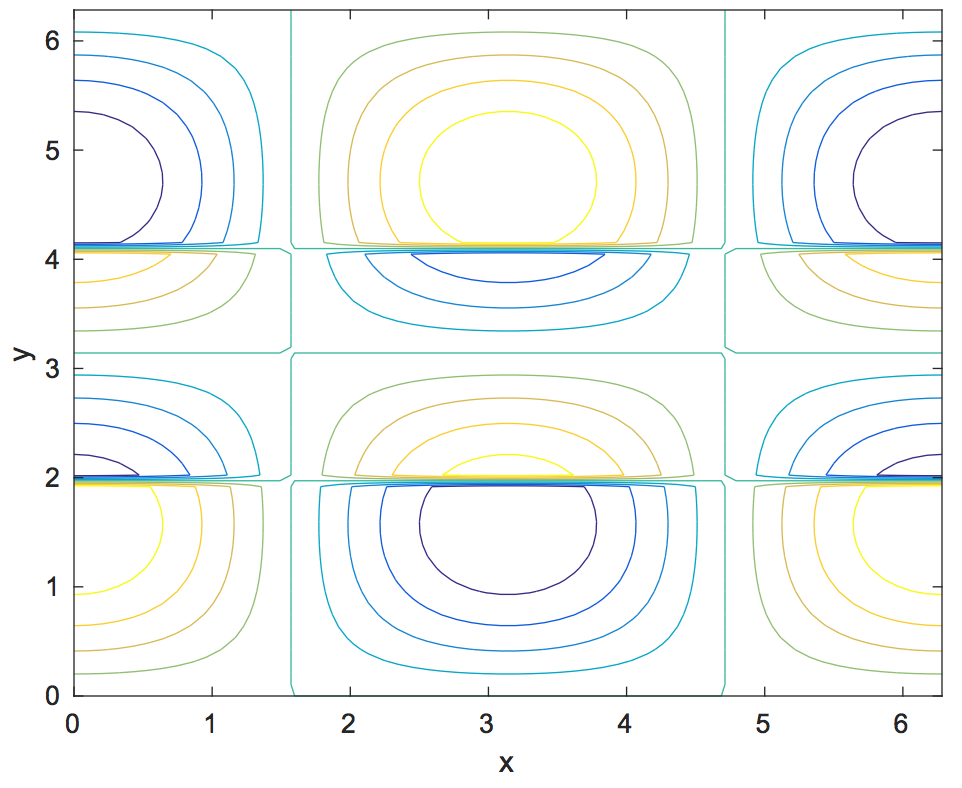
\includegraphics[width=.48\textwidth]{/Users/meganchang/Desktop/Thesis/images/Discontinuous_y_contour.png}}\\
    \caption[Discontinuous Function Used to Test Accuracy of WENO Schemes]{Discontinuous function separated into three parts where the first and final third are defined by the equation $f(x,y)=\cos(x)\sin(y)$, whereas the middle is defined by the negative of that function $f(x,y)=-\cos(x)\sin(y)$. }
  \label{fig:discontinuous_WENO}
\end{figure}

\begin{figure} [!h]
\centering
\subfigure[Mesh: $\phi_x$]{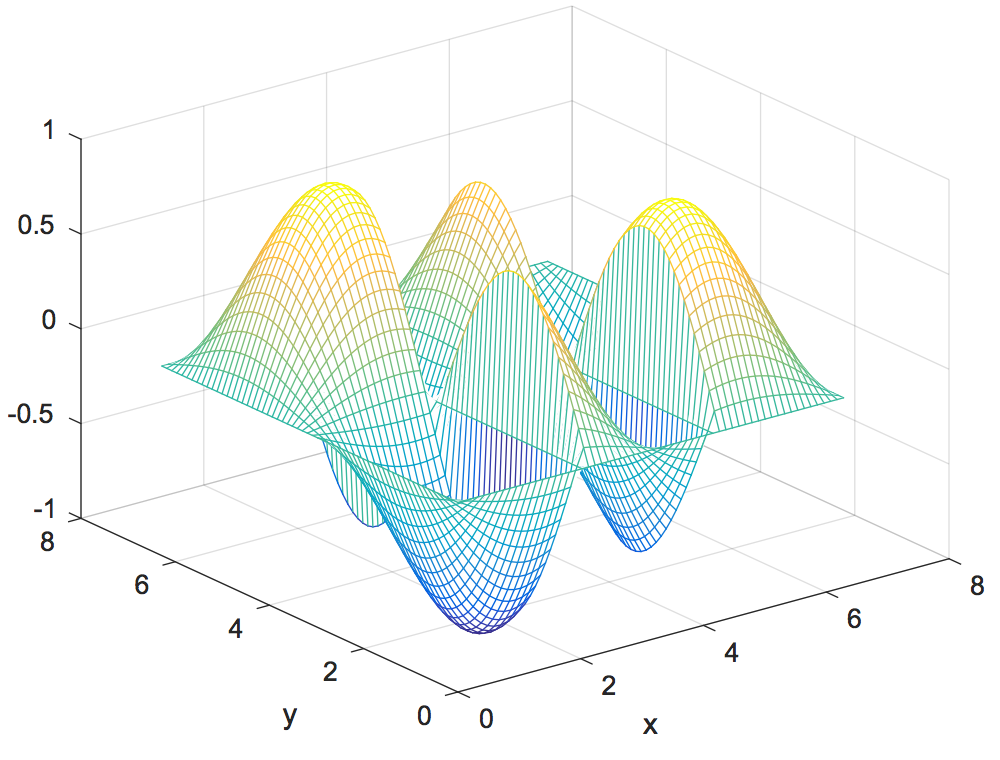
\includegraphics[width=.48\textwidth]{/Users/meganchang/Desktop/Thesis/images/Compute_Dx.png}} \quad
\subfigure[Contour: $\phi_x$]{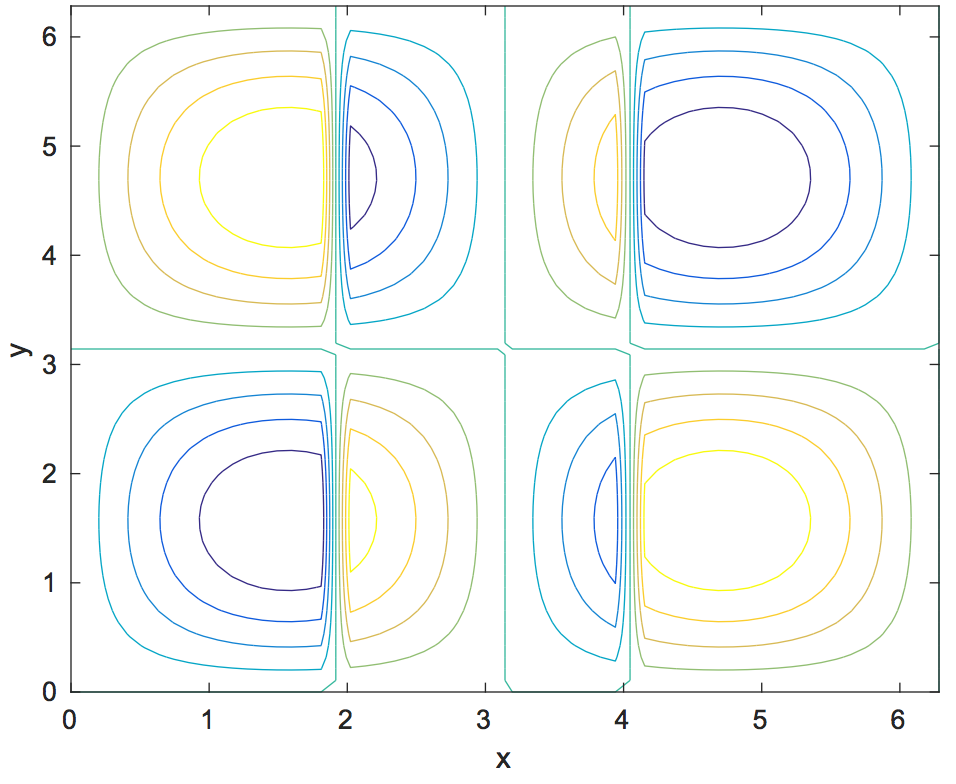
\includegraphics[width=.48\textwidth]{/Users/meganchang/Desktop/Thesis/images/Compute_Dx_contour.png}} \\
\subfigure[Mesh: $\phi_y$]{\includegraphics[width=.48\textwidth]{/Users/meganchang/Desktop/Thesis/images/Compute_Dy.png}} \quad
\subfigure[Contour: $\phi_y$]{\includegraphics[width=.48\textwidth]{/Users/meganchang/Desktop/Thesis/images/Compute_Dy_contour.png}}
    \caption[Non-Oscillatory Results for WENO One-Sided Derivatives]{The derivative $\phi_x$ was calculated using the function $\phi$ discontinuous about $x$, and the derivative $\phi_y$ was calculated using the function $\phi$ discontinuous about $y$ to demonstrate the WENO scheme's ability to produce non-oscillatory results for discontinuous functions. In other schemes, treatment at discontinuities creates oscillatory results in the first derivative calculations. Note that these plots do not include the one row or column of error that does peak due to the discontinuity, which is unavoidable.}
  \label{fig:discontinuous_derivatives}
\end{figure}

\clearpage
\newpage
\begin{table} [!h]
\caption{2D WENO Scheme for Upwind Direction $D_x^+ \phi$}
\label{table:2D_WENO_1}
\centering
\begin{tabular}{c c c c c}
\hline
Grid Resolution  & $L^1$ - error    & Order  & $L^\infty$ - error & Order \\ \hline
81$\times$81          & $6.368 \times 10^{-5}$  &   -    & $6.486 \times 10^{-5}$   &  -  \\
161$\times$161        & $3.848 \times 10^{-6}$  &  4.05  & $8.010 \times 10^{-6}$   & 3.02\\
321$\times$321        & $2.398 \times 10^{-7} $ &  4.00  & $9.634 \times 10^{-7}$   & 3.06\\
\end{tabular}
\end{table}

\begin{table} [!h]
\caption{2D WENO Scheme for Upwind Direction $D_x^- \phi$}
\centering
\begin{tabular}{c c c c c}
\hline
Grid Resolution  & $L^1$ - error    & Order  & $L^\infty$ - error & Order \\ \hline
81$\times$81          & $6.318 \times 10^{-5}$  &   -    & $8.004 \times10^{-5}$   &  -  \\
161$\times$161        & $3.844 \times 10^{-6}$  &  4.04  & $8.508 \times 10^{-6}$   & 3.24\\
321$\times$321        & $2.397 \times 10^{-7} $ &  4.00  & $1.027 \times 10^{-6}$   & 3.05\\
\end{tabular}
\end{table}


\begin{table} [!h]
\caption{2D WENO Scheme for Upwind Direction $D_y^+ \phi$}
\centering
\begin{tabular}{c c c c c}
\hline
Grid Resolution  & $L^1$ - error    & Order  & $L^\infty$ - error & Order \\ \hline
81$\times$81          & $1.114 \times 10^{-4} $ &   -    & $1.087 \times 10^{-4}$   &  -  \\
161$\times$161        & $6.800 \times 10^{-6} $ &  4.03  & $1.354 \times 10^{-5}$   & 3.00\\
321$\times$321        & $4.164 \times 10^{-7} $ &  4.03  & $1.655 \times 10^{-6} $  & 3.03\\
\end{tabular}
\end{table}


\begin{table} [!h]
\caption{2D WENO Scheme for Upwind Direction $D_y^- \phi$}
\label{table:2D_WENO_4}
\centering
\begin{tabular}{c c c c c}
\hline
Grid Resolution  & $L^1$ - error    & Order  & $L^\infty$ - error & Order \\ \hline
81$\times$81          & $1.105 \times 10^{-4}$  &   -    & $1.157 \times 10^{-4} $  &  -  \\
161$\times$161        & $6.792 \times 10^{-6}$  &  4.02  & $1.380 \times 10^{-5}$  & 3.07\\
321$\times$321        & $4.162 \times 10^{-7}$  &  4.03  & $1.690 \times 10^{-6}$   & 3.03\\
\end{tabular}
\end{table}


\section{Total Variation Diminishing Runge-Kutta (TVD RK3) Method}

Now that we have developed a higher-order accurate method to approximate $\phi_x$, we can implement the TVD RK3 method to compute advection using a combination of three Euler steps and two averaging steps 
\begin{equation}  
\begin{aligned}
\frac{\tilde{\phi}^{n+1} - \>\> \phi^n\>\>}{\Delta t} &+\>\>\>\> u^n \>\phi_x^n \>\>\>\>\>\> +\>\>\> v^n \>\phi_y^n \>\>\>\> = 0,\>\>\>\>  \\
\frac{\tilde{\phi}^{n+2} - \tilde{\phi}^{n+1}}{\Delta t} &+ \>\> u^{n+1} \tilde{\phi}_x^{n+1} \>+ v^{n+1} \tilde{\phi}_y^{n+1} \>= 0,\>\>\>  \\
&\tilde{\phi}^{n+\frac{1}{2}} = \frac{3}{4}\phi^{n} + \frac{1}{4} \tilde{\phi}^{n+2},\\
\frac{\tilde{\phi}^{n+\frac{3}{2}} - \tilde{\phi}^{n+\frac{1}{2}}}{\Delta t} &+ u^{n+\frac{1}{2}} \tilde{\phi}_x^{n+\frac{1}{2}} + v^{n+\frac{1}{2}} \tilde{\phi}_y^{n+\frac{1}{2}} = 0,\>\>\>\> \\
&\phi^{n+1} = \frac{1}{3}\phi^{n} + \frac{2}{3} \tilde{\phi}^{n+\frac{3}{2}}, \\
\end{aligned}
\end{equation}\\
where $v_x$ and $v_y$ are the interface velocity components. We find $\phi_x$ and $\phi_y$ using our WENO schemes so that, if $v_x > 0$, we would use $D_x^-$ and if $v_x < 0$, we would use $D_x^+$. Similarly, if $v_y > 0$, we would use $D_y^-$ and if $v_y < 0$, we would use $D_y^+$. Since this is a third-order accurate method, it will be the limiting factor in our advection accuracy (remembering that WENO was up to fifth-order accurate and at minimum, third-order).


\section{Accuracy of the Advection Scheme}

To check the order of accuracy for advection, we use two tests. The first, is the vortex test where we begin with a circular level-set
\begin{equation}
\phi = (x-0.5)^2 + (y-0.75)^2 - 0.15^2,
\end{equation}
on a domain $\Omega$ = [0,1]$^2$ and deform it for 1 second using a vortex, defined by the conservative velocity field:
\begin{equation}
\begin{aligned}
	v_x(x,y) &= -\sin^2(\pi x) \sin(2\pi y),\\
	v_y(x,y)  &= \>\>\>\sin^2(\pi y) \sin(2\pi x),
\end{aligned}	
\end{equation}
so that it takes the shape shown in Figure \ref{fig:vortex_and_overlap}(a). We then run our numerical simulation for the same amount of time (1 second) with the reverse velocities $-v_x$ and $-v_y$ so that our zero level-set returns to its original position and shape. Then, we can compare the initial and final zero level-sets to ensure that our numerical interface is capable of undergoing dramatic deformations while still upholding the law of conservation of mass. In Figure \ref{fig:vortex_and_overlap}(a), there is likely some mass lost at the tail of the level-set deformed by the vortex as it is stretched to thinner degrees. In Figure \ref{fig:vortex_and_overlap}(b), we plot the initial and final zero level-sets to show that there is, indeed, mass loss. However, as we refine our grid, this mass loss becomes negligible as shown in Figure \ref{fig:vortex_101}.

Our numerical scheme for advection maintains between third and fifth-order accuracy as one can see in Table \ref{table:vortex_test}. This is to be expected since we used a third-order accurate method for our time discretization and fifth-order accurate method for our spatial discretization.

\begin{figure}
\centering
\subfigure[Level-set disfigured after vortex has acted on it for 1 second.]{\includegraphics[width=.4\textwidth,height=62mm]{/Users/meganchang/Desktop/Thesis/images/Vortex.png}} \quad
\subfigure[Initial and final level-set after vortex has deformed it in one direction then deformed it in reverse direction.]{\includegraphics[width=.4\textwidth,height=62mm]{/Users/meganchang/Desktop/Thesis/images/Overlap.png}}
\caption[Advection Vortex Test]{We test for mass conservation by distorting the level-set using vortices acting in one direction, then reversing the vortices and comparing the difference between the initial and final zero level-sets. One can clearly see that mass has indeed been lost. We chose a low grid resolution of 41$\times$41 to demonstrate this, but in fact, our program is very good at conserving mass as can be seen in Figure \ref{fig:vortex_101}.}
\label{fig:vortex_and_overlap}
\end{figure}

\begin{figure}
\centering
\includegraphics[width=.4\textwidth,height=62mm]{/Users/meganchang/Desktop/Thesis/images/Vortex_101.png}}
\caption[Negligible Mass Loss During Advection]{Here, we show the same plot as in Figure \ref{fig:vortex_and_overlap}(b), at a higher grid resolution of 101$\times$101. At this grid resolution, one cannot even distinguish the difference between the initial and final zero level-sets, proving that the mass loss is negligible for refined grids.}
\label{fig:vortex_101}
\end{figure}

\begin{table} [ht]
\caption{Advection Vortex Test w/ $\Delta t = 0.5$ min$(\Delta x,\Delta y)/|v|_{max}$ }\label{table:vortex_test}
\centering
\begin{tabular}{c c c c c}
\hline
Grid Resolution & $L^1$ - error    & Order  & $L^{\infty}$ - error & Order \\ \hline
81$\times$81   & $1.352 \times 10^{-4}$  &   -    & $1.100 \times 10^{-3} $  &  -  \\
161$\times$161 &$ 5.966 \times 10^{-6}$  &  4.50  & $1.319 \times 10^{-4}$   & 3.04\\
321$\times$321 & $2.307 \times 10^{-7} $ &  4.69  & $1.090 \times 10^{-5} $  & 3.60\\
\end{tabular}
\end{table}

To be thorough in our testing, we implemented a second test. Here, we advect a periodic level-set given by 
\begin{equation}
\phi(x,y) = \cos(x - x_c)\sin(y-y_c),
\end{equation}
in a domain $\Omega$ = [$-\pi$,$\pi$]$^2$. We use velocities $v_x = 1$ and $v_y = 1$ and a final time $t_\text{final} = 0$, so that we know if the solution ($x_c,y_c$) is initially at (0,0), the final analytical solution will be at (1,1). This test proves our advection solver achieves third-order accuracy as can be seen in Table \ref{table:Advection_Test}.

\begin{table} [ht]
\caption{Advection Test w/ $\Delta t = 0.5 $min$(\Delta x,\Delta y)/|v|_{max}$}
\label{table:Advection_Test}
\centering
\begin{tabular}{c c c c c}
\hline
Grid Resolution & $L^1$ - error    & Order  & $L^{\infty}$ - error & Order \\ \hline
81$\times$81   & $5.204 \times 10^{-4} $ &   -    & $2.054 \times 10^{-5}  $ &  -  \\
161$\times$161 & $6.426 \times 10^{-5} $ &  3.05  & $2.536 \times 10^{-6} $  & 3.05\\
321$\times$321 & $7.961 \times 10^{-6} $ &  3.03  & $3.151 \times 10^{-7}$   & 3.02\\
\end{tabular}
\end{table}

%=== Chapter 6  ============================================
\chapter{Stefan Solver}\label{section:snowflake}

Our first-order accurate Stefan solver calls upon all of the previously discussed functions to simulate crystal growth where the conserved variable $u$ of interest is temperature. Thus, in terms of the heat equation, this diffusion can be thought of as conduction. For example, if you were to hold a metal rod so that one end was in a fire, eventually, through the diffusion of temperature in the metal rod, or the conduction of heat, the rod would burn your hand even if your hand was never near the fire (assuming the diffusion coefficient of the metal was large enough).

We consider an initial level-set describing ice in supercooled water, where supercooled means the water is below freezing point without solidification. We begin by setting the parameters: grid resolution $N$$\times$$N$, diffusion coefficients $D_\text{in}$ and $D_\text{out}$, boundary conditions $u_\gamma$, initial temperature conditions $T^0_\text{in}$ and $T^0_\text{out}$, and initial level-set $\phi^0$. Since our temperature $T$ will be discontinuous about the interface, initially, we must smooth them out using the diffusion function until a steady state is reached whereby $T_\text{in}^0$ and  $T_\text{out}^0$ match at the interface and form a continuous temperature field. We can set $\Delta t = \Delta x$, since our Crank-Nicholson scheme allows it. To be safe, we execute our diffusion code for the same number of iterations as our iterative methods to ensure convergence.

Once, we have defined satisfactory initial conditions for temperature, we can enter our while loop that runs until the final time is reached. The pseudo code below shows the algorithm used to solve our Stefan problem.\\

\ssp
\begin{lstlisting}
while t < tfinal
    
    Third Order Extrapolation of $T_{in}^n$  from $\Omega^-$ into $\Omega^+$
    Third Order Extrapolation of $T_{out}^n$ from $\Omega^+$ into $\Omega^-$ 
    
    Compute velocities $v_x$ and $v_y$
    
    In normal direction at interface:
       Constant Extrapolation of $v_x$ into $\Omega^+$
       Constant Extrapolation of $v_x$ into $\Omega^-$
       Constant Extrapolation of $v_y$ into $\Omega^+$
       Constant Extrapolation of $v_y$ into $\Omega^-$
    
    Compute new time step $\Delta t$ = 0.5min($\Delta x, \Delta y$)/ $|v|_{max}$;   

    Find $\phi^{n+1}$ by advecting $\phi^n$ with interface velocity
    
    Compute anisotropic boundary conditions
    
    Diffusion of $T_{in}^{n+1}$ using $\phi^{n+1}$
    Diffusion of $T_{out}^{n+1}$ using $-\phi^{n+1}$
    
    Reinitialize $\phi^{n+1}$
    
    t = t+dt;
    
end
\end{lstlisting}

\dsp

For each time step, we begin by using our third-order extrapolation method to extrapolate the band of points $T_\text{in}$ and $T_\text{out}$ about the interface. Next, we are ready to calculate the interface velocity $\vec{v}$ using the gradients of temperature at the interface. We use constant extrapolation to make the interface velocity constant in the normal direction to the interface to ensure better behavior of the level-set. For stability purposes, we recalculate the new time step, here, using $\Delta t = 0.5 \text{min}(\Delta x,\Delta y)/|v|_{\text{max}}$. Next, we compute the new level-set $\phi^{n+1}$ by advecting the front with the computed interface velocity. Now, we can calculate the Gibbs-Thomson boundary conditions \eqref{eqn:Gibbs} (discussed later) to impose anisotropic conditions. Then, we call on our diffusion solver to solve in each domain $\Omega^-$ and $\Omega^+$. We use the current extrapolated temperature field $T_\text{in}^n$, $\phi^{n+1}$, $D_\text{in}$ and our boundary conditions to compute $T_\text{in}^{n+1}$ in $\Omega^-$, and use the current extrapolated temperature field $T_\text{out}^n$, $-\phi^{n+1}$, $D_\text{out}$ and our boundary conditions to compute $T_\text{out}^{n+1}$ in $\Omega^+$. Finally, we reinitialize our level-set. To reach the final time, we would repeat this process for the necessary amount of time steps.

To demonstrate some interesting examples of crystal growth, we refer to Gibou's paper [3] on numerically simulating dendritic solidification by imposing anisotropic diffusion. Anisotropy is the property of being directionally dependent, and when applied to simulate the surface tension at the interface, produces dendritic growth. We impose Gibbs-Thomson boundary conditions at the interface defined as
\begin{equation}\label{eqn:Gibbs}
 u_\gamma = u + \epsilon \kappa.
\end{equation}
Here, $\kappa$ is the curvature of the interface ($\kappa = \nabla \cdot \vec{n}$), and $\epsilon_c$ is the surface tension coefficient
\begin{equation}
\epsilon_c = d_0(1-15 \epsilon \cos(4\alpha)),
\end{equation}
where $d_0$ is the anisotropy coefficient, $\epsilon$ is the anisotropy strength, and $\alpha$ is the angle between the normal at the interface and the $x$-axis. This formula represents the standard four-fold anisotropy and allows us to create interesting geometries such as those shown in Figures \ref{fig:snowflake_1} - \ref{fig:snowflake_3}. For each snowflake, we begin with an initial square zero level-set defined by
\begin{equation}
\phi = \text{max}(|x|,|y|) - 0.1 \sqrt{2}
\end{equation}
in a domain $\Omega = [-1.5,1.5]^2$ with grid resolution 200$\times$200. For our time step, we use the restriction $\Delta t = 0.5 \text{min}(\Delta x,\Delta y)/|v|_\text{max}$. We define both diffusion coefficients $D_{\text{in}} = D_{\text{out}} = 0.5$, and initial temperatures $u_\text{in}^0 = 0$, and $u^0_\text{out} = -0.5$. Finally, to induce dendritic growth, we set the anisotropic feature $d_0 = 0.005$ and vary $\epsilon$ to create the three different snowflakes.

One will notice that as the dendrites grow, some merge into each other, which is why the final snowflakes in Figures 6.1(f), 6.2(f), and 6.3(f) have developed holes and gaps in the ice. As we discussed earlier, the level-set method was designed to handle these types of complex topological changes, and indeed, we are able to demonstrate its capabilities in these examples. We include Figure \ref{fig:snowflake_a_crazy} to help observe this phenomenon and better visualize how these dendrites grow along preferred directions. One should also notice the lack of symmetry in the actual snowflake growth. That is to say, despite the symmetry of the grid and initial conditions, the dendrite growths vary on different sides of the initial square crystal. This is due to the anisotropic effects and the highly nonlinear unstable nature of this problem.

In Figure \ref{fig:snowflake_diff_1}, we show the effects of varying the diffusion coefficient on snowflake growth. One will notice that a greater diffusion coefficient will increase the interface velocity so that the snowflake will grow faster.

\begin{figure}
\centering
\subfigure[t = 0.000 s]{\includegraphics[width=.36\textwidth,height=54mm]{/Users/meganchang/Desktop/Thesis/images/Snowflake_Time_0.png}} \quad 
\subfigure[t = 0.005 s]{\includegraphics[width=.35\textwidth]{/Users/meganchang/Desktop/Thesis/images/Snowflake_A_1.png}} \\
\subfigure[t = 0.010 s]{\includegraphics[width=.36\textwidth]{/Users/meganchang/Desktop/Thesis/images/Snowflake_A_2.png}} \quad 
\subfigure[t = 0.015 s]{\includegraphics[width=.36\textwidth]{/Users/meganchang/Desktop/Thesis/images/Snowflake_A_3.png}} \\
\subfigure[t = 0.020 s]{\includegraphics[width=.36\textwidth]{/Users/meganchang/Desktop/Thesis/images/Snowflake_A_4.png}} \quad 
\subfigure[t = 0.025 s]{\includegraphics[width=.36\textwidth]{/Users/meganchang/Desktop/Thesis/images/Snowflake_A_5.png}} \\
\caption[Snowflake Growth A]{Time lapse of snowflake growth on 200$\times$200 grid with $\epsilon = 0.7$.}
  \label{fig:snowflake_1}
\end{figure}

\begin{figure}
\centering
\subfigure[t = 0.000 s]{\includegraphics[width=.36\textwidth,height=54mm]{/Users/meganchang/Desktop/Thesis/images/Snowflake_Time_0.png}} \quad
\subfigure[t = 0.005 s]{\includegraphics[width=.36\textwidth]{/Users/meganchang/Desktop/Thesis/images/Snowflake_B_1.png}} \\
\subfigure[t = 0.010 s]{\includegraphics[width=.36\textwidth]{/Users/meganchang/Desktop/Thesis/images/Snowflake_B_2.png}} \quad
\subfigure[t = 0.015 s]{\includegraphics[width=.36\textwidth]{/Users/meganchang/Desktop/Thesis/images/Snowflake_B_3.png}} \\
\subfigure[t = 0.020 s]{\includegraphics[width=.36\textwidth]{/Users/meganchang/Desktop/Thesis/images/Snowflake_B_4.png}} \quad
\subfigure[t = 0.025 s]{\includegraphics[width=.36\textwidth]{/Users/meganchang/Desktop/Thesis/images/Snowflake_B_5.png}} \\
\caption[Snowflake Growth B]{Time lapse of snowflake growth on 200$\times$200 grid with $\epsilon = 0.6$.}
  \label{fig:snowflake_2}
\end{figure}


\begin{figure}
\centering
\subfigure[t = 0.000 s]{\includegraphics[width=.36\textwidth,height=54mm]{/Users/meganchang/Desktop/Thesis/images/Snowflake_Time_0.png}} \quad
\subfigure[t = 0.010 s]{\includegraphics[width=.36\textwidth]{/Users/meganchang/Desktop/Thesis/images/Snowflake_C_1.png}} \\
\subfigure[t = 0.020 s]{\includegraphics[width=.36\textwidth]{/Users/meganchang/Desktop/Thesis/images/Snowflake_C_2.png}} \quad
\subfigure[t = 0.030 s]{\includegraphics[width=.36\textwidth]{/Users/meganchang/Desktop/Thesis/images/Snowflake_C_3.png}} \\
\subfigure[t = 0.040 s]{\includegraphics[width=.36\textwidth]{/Users/meganchang/Desktop/Thesis/images/Snowflake_C_4.png}} \quad
\subfigure[t = 0.050 s]{\includegraphics[width=.36\textwidth]{/Users/meganchang/Desktop/Thesis/images/Snowflake_C_5.png}} \\
\caption[Snowflake Growth C]{Time lapse of snowflake growth on 200$\times$200 with $\epsilon = 0.3$.}
  \label{fig:snowflake_3}
\end{figure}

\begin{figure}
\centering
\includegraphics[width=.48\textwidth]{/Users/meganchang/Desktop/Thesis/images/Snowflake_Ayo.png}}
\caption[Dendritic Growth Behavior]{Here, we include many more time step renderings all plotted on the same figure. In this figure, it is highly apparent that the dendrites grow along preferred directions due to the anisotropic boundary conditions.  One can clearly see how the holes begin to develop from dendrites growing and merging into each other. This is the same snowflake as the one shown in Figure \ref{fig:snowflake_1} (i.e. Snowflake Growth A).}
\label{fig:snowflake_a_crazy}
\end{figure}

\begin{figure}
\centering
\subfigure[D = 3]{\includegraphics[width=.4\textwidth]{/Users/meganchang/Desktop/Thesis/images/Snowflake_Diffusion_1.png}} \quad
\subfigure[D = 1]{\includegraphics[width=.4\textwidth]{/Users/meganchang/Desktop/Thesis/images/Snowflake_Diffusion_2.png}} \\
\subfigure[D = 3]{\includegraphics[width=.4\textwidth]{/Users/meganchang/Desktop/Thesis/images/Snowflake_Diffusion_3.png}} \quad
\subfigure[D = 1]{\includegraphics[width=.4\textwidth]{/Users/meganchang/Desktop/Thesis/images/Snowflake_Diffusion_4.png}} \\
\caption[Diffusion Effects on Snowflake Growth]{Effects of diffusion coefficient on snowflake growth. Here, we show the growth every 0.001 seconds for a final time of 0.05 seconds on a grid size 200$\times$200 with the same supercooled system as the snowflakes and no anisotropic effects. We vary the diffusion coefficient from 1 to 3 for the two different level-set shapes to demonstrate how the interface velocity increases with the diffusion coefficient.}
\label{fig:snowflake_diff_1}
\end{figure}

%=== Chapter 7  ============================================
\chapter{Efficient Matlab Implementation}\label{section:gaining_efficiency_0}

We have already discussed a few strategies used to make our code more powerful such as using sparse matrices to reduce memory storage. Now, we will discuss some of the steps taken to improve computational efficiency. There were two areas where significant improvements were made: the diffusion solver and the iterative methods. (Please note that in the following subsections, a 64-bit Linux Ubuntu OS was used with 62.8 GiB of memory and an Intel Xeon(R) CPU e5-1650 v4 @ 3.60GHz $\times$ 12 processor.

\section{Building a Compact Diffusion Matrix}\label{section:gaining_efficiency_1}

The original diffusion function created a linear equation $\boldsymbol{A}\vec{u}^{\>n+1} = \vec{f}\>(\vec{u}^{\>n},BC^{n+1})$ for each grid point in the entire domain $\Omega$, which equates to a diffusion matrix size of 40,000$\times$40,000 for a grid resolution of 200$\times$200. This means the program was creating identity equations at grid points that fell on the interface where the solution was known (i.e. $u^{n+1}_{i,j} = BC^{n+1}_{i,j}$), and at grid points in $\Omega^+$ where the solution was invalid and, therefore, unused (i.e. $u^{n+1}_{i,j} = 0$). We used this method initially because it was easy to implement and seemed reasonably efficient for smaller grid resolutions. However, as we began to refine our grid, this method was no longer effective.

To demonstrate the gain in efficiency, we include Table \ref{table:diffusion_efficiency_grid_size}, which executes the diffusion program a total of 275 times to simulate 275 time steps. We use this number for comparison throughout the efficiency study so that we can make a reasonable comparison of the comprehensive Stefan solvers at the end. We used a circular level-set with a radius of 0.5 in a domain $[-1,1]^2$ using various grid resolutions to show the impact of our improved efficiency. (However, keep in mind that as the grid resolution increases, the time step shrinks. Thus, as one refines the grid, many more time steps would be required to reach the same final time.) We included the time elapsed (in seconds) to execute each program, as well as the percent time reduction, which is calculated as (1 - New Time/Old Time). Notice, as the grid size increases, percent time reduction increases, as well, so that for a grid size 100$\times$100, the new diffusion solver is 25.5 times faster, and with a grid resolution of 500$\times$500, the new diffusion solver is 495 times faster than the original scheme. This increase in efficiency has to do with the growing amount of identity equations which our old solver had to compute. 

\begin{table} [ht]
\caption{Diffusion Program Efficiency for Various Grid Resolutions}
\label{table:diffusion_efficiency_grid_size}
\centering
\begin{tabular}{c c d{5.0} d{2.2} c}
\hline
Grid Resolution & \multicolumn{1}{c}{Old Time(s)} & \multicolumn{1}{c}{New Time(s)} & \multicolumn{1}{c}{$\%$ Time Reduction} \\ \hline
100$\times$100  & 30     &  1.16   & 96.08\% \\
200$\times$200  & 378    &  5.22   & 98.62\% \\
300$\times$300  & 2,025  &  12.05  & 99.41\% \\
400$\times$400  & 6,909  &  21.56  & 99.69\% \\
500$\times$500  & 17,552 &  35.42  & 99.80\% \\
\end{tabular}
\end{table}

To avoid creating thousands of identity equations, we made $\vec{u}^{\>n+1}$ contain only points in $\Omega^-$ in our new diffusion solver. This required use of the ghost value method. Consider, for example, Figure \ref{fig:sample_grid_diffusion_faster}.

\begin{figure}[h]
\centering
\includegraphics[width=.48\textwidth]{/Users/meganchang/Desktop/Thesis/images/Diffusion_Faster.png}
\caption[Diffusion Efficiency Sample Grid]{Consider this grid with ten points in a 2$\times$5 arrangement. For this system, we have four points in $\Omega^+$ that we do not want to compute, four points at the interface with known boundary condition values, and only two points that need to be solved for.}
\label{fig:sample_grid_diffusion_faster}
\end{figure}

For such a case, our old diffusion solver would create an implicit system of linear equations $\boldsymbol{A}\vec{u}^{\>n+1} = \vec{f}\>(\vec{u}^{\>n},BC^{n+1})$ shown in matrix form below:

\dhalfsp
\begin{equation}
\begin{bmatrix}
1 & 0 & 0 & 0 & 0 & 0 & 0 & 0 & 0 & 0\\
0 & 1 & 0 & 0 & 0 & 0 & 0 & 0 & 0 & 0\\
0 & \color{red} \textbf{L} & \color{red} \textbf{C} & \color{red} \textbf{R} & 0 & 0 & 0 & \color{red} \textbf{B}  & 0 & 0\\
0 & 0 & 0 & 1 & 0 & 0 & 0 & 0 & 0 & 0\\
0 & 0 & 0 & 0 & 1 & 0 & 0 & 0 & 0 & 0\\
0 & 0 & 0 & 0 & 0 & 1 & 0 & 0 & 0 & 0\\
0 & 0 & 0 & 0 & 0 & 0 & 1 & 0 & 0 & 0\\
0 & 0 & \color{red} \textbf{A} & 0 & 0 & 0 & \color{red} \textbf{L} & \color{red} \textbf{C} & \color{red} \textbf{R} & 0\\
0 & 0 & 0 & 0 & 0 & 0 & 0 & 0 & 1 & 0\\
0 & 0 & 0 & 0 & 0 & 0 & 0 & 0 & 0 & 1\\
\end{bmatrix}
\begin{bmatrix}
u^{n+1}_{1,1}\\
u^{n+1}_{2,1}\\
u^{n+1}_{3,1}\\
u^{n+1}_{4,1}\\
u^{n+1}_{5,1}\\
u^{n+1}_{1,2}\\
u^{n+1}_{2,2}\\
u^{n+1}_{3,2}\\
u^{n+1}_{4,2}\\
u^{n+1}_{5,2}\\
\end{bmatrix} =
\begin{bmatrix}
0\\
BC^{n+1}_{2,1}\\
f(u^n)_{3,1}\\
BC^{n+1}_{4,1}\\
0\\
0\\
BC^{n+1}_{2,2}\\
f(u^n)_{3,2}\\
BC^{n+1}_{4,2}\\
0\\
\end{bmatrix},
\end{equation}
\dsp
where we filled our RHS vector with zeroes for points outside of $\Omega^-$, Dirichlet boundary conditions where applicable, and $f(u^n)$ to represent some \textbf{known} function of $u^n$. The non-trivial values have been highlighted so one can quickly identify the equations that are non-trivial. In this example, eight of the ten rows are identity equations. The new diffusion solver removes all these trivial rows so that we are left solving only for the two unknowns:
\begin{equation}
\begin{bmatrix}
\textbf{C} & \textbf{B}\\
\textbf{A} & \textbf{C}
\end{bmatrix}
\begin{bmatrix}
u^{n+1}_{3,1}\\
u^{n+1}_{3,2}
\end{bmatrix} = 
\begin{bmatrix}
f(u^{n})_{3,1} - \textbf{L} \> BC^{n+1}_{2,1} - \textbf{R} \> BC^{n+1}_{4,1}\\
f(u^{n})_{3,2} - \textbf{L} \> BC^{n+1}_{2,2} - \textbf{R} \> BC^{n+1}_{4,2}
\end{bmatrix}.
\end{equation}
This matrix is stripped of all lines associated with the known values in the previously used $\vec{u}^{\>n+1}$. One can imagine this by considering the first line of the matrix. We do not want to compute $u^{n+1}_{1,1}$, so we strike the top row and leftmost column from the matrix as shown in Figure \ref{fig:ghost_point_matrix}. This does not affect any other equation since all elements off the diagonal are zero. Next, we move to the second value in our vector: $u^{n+1}_{2,1}$. Here, we notice there is a non-zero element off the diagonal. When this occurs, we must implement the ghost value method so that our linear equation is still valid. Thus, we would move the value L$u^{n+1}_{2,1}$ to the RHS vector by subtracting it.

\begin{figure}[h]
\centering
\includegraphics[width=.85\textwidth]{/Users/meganchang/Desktop/Thesis/images/Ghost_Point_Matrix.png}
\caption[How Ghost Points Work]{Ghost Point Added to the RHS to account for the element $L$ no longer included in the matrix.}
\label{fig:ghost_point_matrix}
\end{figure}

Another way to consider this is by looking at the equation itself outside of matrix form. For the third line, we would end up with the linear equation:
\begin{equation}
\begin{aligned}
\textbf{L} \> BC^{n+1}_{2,1} + \textbf{C} \> u^{n+1}_{3,1} + \textbf{R} \> BC^{n+1}_{4,1} + \textbf{B} \> u^{n+1}_{3,2} = f(u^{n})_{3,1}.
\end{aligned}
\end{equation}
Moving all our knowns to the RHS, we acquire this rearranged equation:
\begin{equation}
\begin{aligned}
\textbf{C} \> u^{n+1}_{3,1} + \textbf{B} \> u^{n+1}_{3,2} = f(u^{n})_{3,1} - \textbf{L} \> BC^{n+1}_{2,1} - \textbf{R} \> BC^{n+1}_{4,1}.
\end{aligned}
\end{equation}
Note, Figure \ref{fig:ghost_point_matrix} is simply provided for a visual understanding of how one can transform the original 10$\times$10 matrix into the new 2$\times$2 matrix. However, in its actual implementation, the new diffusion program skips the generation of the identity equations, so that it only ever builds the concise compact matrix you see in the end, adding the ghost values to the RHS on the fly. This is how our new diffusion solver gains its efficiency over the old diffusion solver.

\section{Computing First-Order Directional Derivatives}\label{section:efficiency_2}

In this thesis, we develop higher-order accurate one-sided finite difference schemes called the WENO schemes. These sacrifice computational efficiency for accuracy, making them highly advantageous for a process like advection where they are only called upon six times, but become cumbersome in iterative methods.
 
In our Stefan solver, we use three iterative methods, which each require a minimum number of iterations to propagate the solution out sufficiently far. During these iterations, the solution will continue to converge to comparable accuracies, regardless of the accuracy of the directional derivatives. For all three snowflakes shown in Figures \ref{fig:snowflake_1} -  \ref{fig:snowflake_3}, we used 50 iterations of reinitialization; 160 iterations of constant extrapolation (i.e. 40 iterations to extrapolate $v_x$ and $v_y$ in both normal directions); and 80 iterations of third-order extrapolation (i.e. 40 iterations to extrapolate $T_{in}$ and $T_{out}$ in a band around the interface). Recall that these iterations occur at every time step, and with each iteration, we calculate all four directional derivatives. Thus, over the course of 275 time steps, we call upon our directional derivatives a grand total of 55,000 times for reinitialization, 176,000 times for constant extrapolation, and 88,000 times for third-order extrapolation. Thus, we require a cheaper method for computing directional derivatives which we developed in equation \eqref{eqn:directional_derivatives}. Tables \ref{table:reinitialization_efficiency} - \ref{table:third_order_efficiency} demonstrate the efficiency gained when we use first-order schemes in place of the WENO schemes.

\begin{table} [ht]
\caption{Reinitialization Efficiency for Various Grid Resolutions}
\label{table:reinitialization_efficiency}
\centering
\begin{tabular}{c d{6.0} d{5.0} d{2.2} c}
\hline
Grid Resolution  &  \multicolumn{1}{c}{Old Time(s)} & \multicolumn{1}{c}{New Time(s)} & \multicolumn{1}{c}{$\%$ Time Reduction} \\ \hline
100$\times$100  &  635     &  9.39    & 98.52\% \\
200$\times$200  &  2,551   &  36.60   & 98.56\% \\
300$\times$300  &  5,764   &  79.64   & 98.62\% \\
400$\times$400  &  9,708   &  139.79  & 98.56\% \\
500$\times$500  &  15,156  &  221.99  & 98.54\% \\
\end{tabular}
\end{table}


\begin{table} [ht]
\caption{Constant Extrapolation Efficiency for Various Grid Resolutions}
\label{table:constant_extrapolation_efficiency}
\centering
\begin{tabular}{c d{6.0} d{5.0} d{2.2} c}
\hline
Grid Resolution &   \multicolumn{1}{c}{Old Time(s)} & \multicolumn{1}{c}{New Time(s)} & \multicolumn{1}{c}{$\%$ Time Reduction} \\ \hline
100$\times$100  &  2,957    &  21.44   & 99.28\% \\
200$\times$200  &  11,462   &  80.49   & 99.30\% \\
300$\times$300  &  25,818   &  177.79  & 99.31\% \\
400$\times$400  &  49,207   &  321.36  & 99.35\% \\
500$\times$500  & 75,783   &  515.61  & 99.32\% \\
\end{tabular}
\end{table}

\begin{table} [ht]
\caption{Third-Order Accuracy Efficiency for Various Grid Resolutions}
\label{table:third_order_efficiency}
\centering
\begin{tabular}{c d{6.0} d{5.0} d{2.2} c}
\hline
Grid Resolution &  \multicolumn{1}{c}{Old Time(s)} & \multicolumn{1}{c}{New Time(s)} & \multicolumn{1}{c}{$\%$ Time Reduction} \\ \hline
100$\times$100  &  2,893     &  32.41    & 98.88\% \\
200$\times$200  &  11,497    &  123.50   & 98.93\% \\
300$\times$300  &  27,699    &  274.32   & 99.01\% \\
400$\times$400  &  46,730    &  484.58   & 98.98\% \\
500$\times$500  &  77,003    &  760.39   & 99.01\% \\
\end{tabular}
\end{table}

Table \ref{table:snowflake_time} shows the time it would take for the diffusion and iterative methods of the Stefan solver to execute 275 time steps for a circular level-set with radius 0.5 in a 200$\times$200 grid to demonstrate the efficiency we have gained.

\begin{table} [ht]
\caption{Time to Make the Snowflake}
\label{table:snowflake_time}
\centering
\begin{tabular}{c d{5.0} d{2.2} c}
\hline
Method &  \multicolumn{1}{c}{Old Time(s)} & \multicolumn{1}{c}{New Time(s)} & \multicolumn{1}{c}{$\%$ Time Reduction} \\ \hline
Diffusion                 & 378       &  5.22     & 98.62\% \\
Reinitialization          & 2,551     &  36.60    & 98.56\% \\
Constant Extrapolation    & 11,462    &  80.49    & 99.30\% \\
Third-Order Extrapolation & 11,497    &  123.50   & 98.93\% \\
Total Time                & 25,888    &  245.81   & 99.05\% \\
\end{tabular}
\end{table}

I have also included a simulation run at a higher grid resolution of 500$\times$500 to demonstrate the significance of this speed enhancement. With the new methods, it takes 35 minutes to execute 275 time steps, whereas with the old methods, it takes three days.

\begin{table} [ht]
\caption{Time for 275 time steps at Higher Grid Resolution}
\label{table:snowflake_time_500}
\centering
\begin{tabular}{c d{5.0} d{2.2} c}
\hline
Method &  \multicolumn{1}{c}{Old Time(s)} & \multicolumn{1}{c}{New Time(s)} & \multicolumn{1}{c}{$\%$ Time Reduction} \\ \hline
Diffusion                 & 17,552    &  35.42    & 99.80\% \\
Reinitialization          & 15,156    &  221.99   & 98.54\% \\
Constant Extrapolation    & 75,783    &  515.61   & 99.32\% \\
Third-Order Extrapolation & 77,003    &  760.39   & 99.01\% \\
Total Time                & 254,444   &  2,055.23 & 99.19\% \\
\end{tabular}
\end{table}

%=== Chapter 8  ============================================
\chapter{Closing Thoughts}

The Stefan problem is a complicated free boundary problem with no analytical solutions. Therefore, we developed a numerical method to allow us to analyze dendritic crystal growth. As we discussed in Section \ref{section:Interface_Velocity}, our Stefan solver is first-order accurate overall because of the interface velocity calculation. Using quadratic extrapolation of the ghost values gives us a second-order accurate solution \textbf{and} second-order accurate derivative. In numerical analysis, this is called super convergence because it converges faster than one would expect. When we use linear extrapolation instead, we maintain the second-order accurate solution, but lose one order of accuracy in our gradient. However, this allows us to have symmetric discretization, which in turn enables us to use much faster solvers like PCG, whereas with non-symmetric discretization, we are forced to use slow solvers like Gauss-Seidel. With numerical methods, the coder must sometimes choose what to prioritize. In this thesis, we chose to prioritize solver efficiency over one order of accuracy because the non-symmetric discretization is simply too computationally expensive. As we refined the grid, it would have become computationally prohibitive, and grid refinement is unavoidable to capture dendritic structures. Thus, we chose to build a simpler, but faster model that would allow us to execute many more studies in a shorter amount of time, as well as study higher grid resolutions.

We develop higher-order tools like third-order extrapolation and up to fifth-order WENO methods so that error does not compound throughout the solver and further reduce our precision. Further, our solver was built with higher-order dimensions in mind. Tools like the level-set can easily be extended to a three-dimensional problem by simply adding an extra index. Additionally, the entire code can readily be used with adaptive grid meshing as shown by Chen, Min, and Gibou in [2]. Thus, one advantage of the solver presented in this thesis, is that it provides a solid foundation for modeling the Stefan problem, that can be built upon easily.

We touched upon some reasons why the Stefan problem is a significant problem to study, earlier, and expand upon it here, as well as how our code could be used as a simple model for some of these important applications.

The word dendrites comes from the Greek word for tree, $dendron$. Metallurgists began using the term to describe alloy growth after observing tree-like branch structures in the freshly cast metal mixtures. An alloy is a mixture of metals like brass (copper and zinc) or mixture of metal and elements like steel or stainless steel (iron and carbon). Under a powerful microscope, an alloy appears to be made up of millions of tiny metallic snowflakes growing around and into each other. This is because as molten metal freezes, crystals grow faster along energetically favorable crystallographic directions. 

Metallurgists discovered that this dendritic crystal growth played an enormous role in determining the alloy properties, including: softness, malleability, elasticity, load-carrying ability, heat and electricity conductance, and how easily it can be welded to another piece of metal - to name a few. All of these properties directly correlated to the shape, size, and speed of the dendritic growth. Thus, numerical simulations are a valuable tool for predicting how different conditions will affect these growth factors and give rise to the desired attributes [8]. For instance, smaller dendrites, which are typically produced by rapid cooling cycles, generally lead to higher ductility. Whereas, long dendrites can provide a ready path for corrosive fluid to penetrate. Thus, one might use the numerical simulations to identify the ideal conditions that would minimize dendrite length.

One example of how this is useful is that it allows us to improve the recipe for materials like superalloys - high strength materials that can perform at extremely high temperatures. They are used in the construction of turbine engines, rocket engines, and power plants because the rule in energy efficiency is that the hotter you can burn fuel, the more energy you get out of it, and thus, the less fuel you need to use. This means superalloys increase energy efficiency and reduce pollution. Currently, superalloys can perform at temperatures over 650 degrees Celcius, and each year this number gets a little higher as they improve the recipe using simulations like the one presented in this thesis to determine the ideal conditions for producing superalloys.

Another important application for analyzing the Stefan problem is in medicine. The diffusion-reaction model has long been used to study cancer invasion [9] whereby we can observe the phase transition of healthy cells into cancer cells via the diffusion of oxygen and other nutrients. Diffusion-reaction models have allowed scientists and doctors to better understand the underlying mechanisms that govern the destruction of normal tissues by metastatic cancer, and map the interactions between tumor cells and normal cells at the tumor-host interface which significantly influences the progression of invasive cancer. Thus, numerical simulations can give us valuable insight into cancer cell growth and what can be done to slow down and treat metastatic cancer invasion. Note, this model does not necessarily display dendritic growth behavior. However, since we know our solver is capable of modeling the more complicated dendritic growth, we know that it is well equipped to study most diffusion-dominated problems which are characterized by simpler growth behaviors.

%=== Appendix ============================================
%\appendix

%\dsp

%\chapter{Appendix Title }{\label{appendix:a}}
%\begin{section}{Section Title}

%Appendicitis

%\end{section}
%\end{mainmatter}

%----- Bibliography ----------------
\ssp
\newpage
%\bibliographystyle{JHEP3}
%\bibliography
\chapter{References}

\parindent[1] F. Gibou, R. Fedkiw, L.Cheng, and M. Kang, A second-order-accurate symmetric discretization of the poisson equation on irregular domains, \textit{Journal of Computational Physics}, 205-227 (2000).\\

[2] C. Min and F. Gibou, A second-order-accurate level-set method on non-graded adaptive cartesian grids, \textit{Journal of Computational Physics}, 200-321 (2006).\\

[3] F. Gibou, R. Fedkiw, R. Caflisch, and S. Osher, A level-set approach for the numerical simulation of dendritic growth, \textit{Journal of Scientific Computing}, 183-199 (2002).\\

[4] M. Sussman, P. Smereka, and S.Osher, A level set approach for computing solutions in incompressible two-phase flow, \textit{Journal of Computational Physics}, 146-159 (1994).\\

[5] T. Aslam, A partial differential equation approach to multidimensional extrapolation, \textit{Journal of Computational Physics}, 349-355 (2004).\\

[6] X. Liu, S. Osher, T. Chan, Weighted essentially non-oscillatory schemes, \textit{Journal of Computational Physics}, 200-212 (1994).\\

[7] H. Chen, C. Min, F. Gibou, A numerical scheme for the Stefan problem on adaptive Cartesian grids with supralinear convergence rate, \textit{Journal of Computational Physics}, 5803-5818 (2009).\\

[8] W.L. George and J.A. Warren, A parallel 3D dendritic growth simulator using the phase-field method, \textit{Journal of Computational Physics}, 264-283 (2002).\\

[9] R.A. Getenby and E.T. Gawlinski, A reaction-diffusion model of cancer invasion, \textit{Journal of Cancer Research}, 5745-5753 (1996).\\

\end{document} 
